\documentclass[a4paper,12pt]{article}

\usepackage[utf8]{inputenc}      % Кодировка документа
\usepackage[T2A]{fontenc}        % Поддержка русских символов
\usepackage[russian]{babel}      % Локализация на русский язык
\usepackage{amsmath, amsthm, amssymb} % Математические пакеты
\usepackage{geometry}            % Настройка полей страницы
\usepackage{chngcntr}            % Для перенумерации определений и теорем по секциям
\usepackage{tikz}
\usetikzlibrary{shapes, arrows, positioning}
\usepackage{verbatim}
\usepackage{listings}
\usepackage{xcolor} % Для настройки цветов (опционально)

\lstset{
    language=SQL,                  % Язык программирования
    basicstyle=\ttfamily\small,    % Размер и стиль шрифта
    keywordstyle=\color{blue}\bfseries, % Стиль ключевых слов
    commentstyle=\color{gray},     % Стиль комментариев
    stringstyle=\color{red},       % Стиль строковых литералов
    breaklines=true,               % Перенос строк
    numbers=left,                  % Нумерация строк слева
    numberstyle=\tiny\color{gray}, % Стиль нумерации строк
    stepnumber=1,                  % Шаг нумерации
    showstringspaces=false          % Не показывать пробелы в строках
}
\geometry{left=3cm, right=3cm, top=2cm, bottom=2cm}

% Определение окружений для теорем, определений и лемм
\newtheorem{definition}{Определение}
\newtheorem{theorem}{Теорема}
\newtheorem{lemma}{Лемма}

% Нумерация определений, теорем и лемм будет сбрасываться в каждой секции (вопросе)
\counterwithin{definition}{section}
\counterwithin{theorem}{section}
\counterwithin{lemma}{section}

% Определение стилей TikZ для ER-диаграмм
\tikzstyle{entity} = [
    rectangle,
    draw=black,
    thick,
    minimum width=2.5cm,
    minimum height=1cm,
    text centered
]

\tikzstyle{attribute} = [
    ellipse,
    draw=black,
    thick,
    minimum width=2cm,
    minimum height=1cm,
    text centered
]

\tikzstyle{relationship} = [
    diamond,
    draw=black,
    thick,
    minimum width=2cm,
    minimum height=1cm,
    text centered
]

\tikzstyle{inherit} = [
    rectangle,
    draw=black,
    thick,
    dashed,
    minimum width=2.5cm,
    minimum height=1cm,
    text centered
]

\tikzstyle{line} = [
    draw,
    -latex
]

\begin{document}

% Начало вопросов
\section{Файл, файловая система. Особенности организации устройств внешней памяти на магнитных дисках. Структуры файлов на дисках. Классификация файловых систем. Основные подходы к защите файловых систем.}

\textbf{Файл} — именованная область внешней памяти, в которую можно записывать и из которой можно считывать данные. \textbf{Файловая система} (ФС) — программная система, управляющая файлами и архивом файлов, хранящимся во внешней памяти.

\textbf{Особенности организации устройств внешней памяти на магнитных дисках}:

\begin{itemize}
    \item \textbf{Жесткие магнитные диски} обеспечивают быстрый произвольный доступ к данным и большую емкость хранения за счет нескольких магнитных поверхностей.
    \item \textbf{Структура диска}:
    \begin{itemize}
        \item Диск состоит из пакета магнитных пластин с радиально двигающимися головками.
        \item Каждое положение головок соответствует цилиндру, содержащему дорожки на всех поверхностях.
    \end{itemize}
    \item \textbf{Доступ к данным} включает:
    \begin{itemize}
        \item \textit{Подвод головок} ($t_{\text{пг}}$): время перемещения головок к нужному цилиндру (самое длительное).
        \item \textit{Поиск блока на дорожке} ($t_{\text{пб}}$): ожидание нужного блока при вращении диска.
        \item \textit{Обмен данными} ($t_{\text{об}}$): чтение или запись блока (самое короткое время).
    \end{itemize}
\end{itemize}

\textbf{Структуры файлов на дисках}:

\begin{itemize}
    \item Файлы состоят из последовательностей блоков, которые отображаются на физические блоки диска.
    \item Размер логических блоков обычно равен или кратен размеру физического блока диска.
    \item Два подхода к представлению файлов:
    \begin{itemize}
        \item \textbf{Последовательность записей}: файлы как набор записей фиксированной или переменной длины.
        \item \textbf{Последовательность байтов}: файлы как непрерывная последовательность байтов (как в UNIX).
    \end{itemize}
\end{itemize}

\textbf{Классификация файловых систем}:

\begin{itemize}
    \item По логической структуре и именованию файлов:
    \begin{itemize}
        \item \textbf{Изолированные ФС}: каждый архив файлов расположен на отдельном логическом диске; полные имена файлов начинаются с имени устройства.
        \item \textbf{Централизованные ФС}: единое дерево каталогов, физически распределенное по всем устройствам; имена файлов начинаются с корневого каталога.
        \item \textbf{Гибридные подходы} (например, UNIX): комбинация изолированных и централизованных систем через механизм монтирования.
    \end{itemize}
\end{itemize}

\textbf{Основные подходы к защите файловых систем}:

\begin{itemize}
    \item \textbf{Мандатный способ защиты}: каждому пользователю назначаются права на каждый файл (сложно и ресурсоемко).
    \item \textbf{Дискреционный способ защиты} (как в UNIX):
    \begin{itemize}
        \item Пользователи имеют идентификаторы пользователя и группы.
        \item Для каждого файла определяются права доступа для владельца, группы и остальных (чтение, запись, выполнение).
        \item Обеспечивает компактность и быструю проверку прав доступа.
    \end{itemize}
\end{itemize}

\section{Возможности и области применения файловых систем. Сравнение ФС и СУБД по обеспечению требований со стороны информационных систем: согласованность данных, языки запросов, восстановление согласованного состояния после сбоев, реальный режим мультидоступа.}

\textbf{Возможности и области применения файловых систем}:

\begin{itemize}
    \item Хранение слабо структурированной информации, где структура данных определяется прикладными программами (текстовые редакторы, компиляторы).
    \item Предоставление базовых функций: распределение памяти, именование файлов, авторизация доступа, поддержка многопользовательского режима.
    \item Подходят для приложений с простыми структурами данных и последовательным доступом.
\end{itemize}

\textbf{Сравнение ФС и СУБД по требованиям информационных систем}:

\begin{itemize}
    \item \textbf{Согласованность данных}:
    \begin{itemize}
        \item \textbf{ФС}: не обеспечивают автоматическую согласованность данных между файлами; ответственность лежит на приложениях.
        \item \textbf{СУБД}: поддерживают целостность данных через механизмы ограничений и транзакций, обеспечивая согласованное состояние базы данных.
    \end{itemize}
    \item \textbf{Языки запросов}:
    \begin{itemize}
        \item \textbf{ФС}: отсутствуют высокоуровневые языки запросов; доступ к данным осуществляется через низкоуровневые операции ввода-вывода.
        \item \textbf{СУБД}: предоставляют декларативные языки запросов (например, SQL), позволяющие эффективно и удобно манипулировать данными.
    \end{itemize}
    \item \textbf{Восстановление после сбоев}:
    \begin{itemize}
        \item \textbf{ФС}: ограниченная поддержка; приложения должны самостоятельно обеспечивать восстановление, что может привести к рассогласованности данных.
        \item \textbf{СУБД}: имеют встроенные механизмы журнализации и восстановления, позволяющие вернуть базу данных в согласованное состояние после сбоев.
    \end{itemize}
    \item \textbf{Реальный режим мультидоступа}:
    \begin{itemize}
        \item \textbf{ФС}: базовая синхронизация доступа через блокировки файлов; при записи файлы могут быть недоступны другим пользователям.
        \item \textbf{СУБД}: реализуют тонкую синхронизацию на уровне записей или даже полей, позволяя множеству пользователей одновременно работать с данными без конфликтов.
    \end{itemize}
\end{itemize}

\section{СУБД. Основные функции СУБД. Типовая организация современной СУБД.}

\textbf{Основные функции СУБД}:

\begin{itemize}
    \item \textbf{Управление согласованными данными во внешней памяти}:
    \begin{itemize}
        \item Поддержка структур хранения данных, метаданных и служебной информации (индексов).
        \item Обеспечение логической целостности данных.
    \end{itemize}
    \item \textbf{Управление буферами оперативной памяти}:
    \begin{itemize}
        \item Кэширование данных для повышения скорости доступа.
        \item Собственные алгоритмы замены буферов для эффективной работы.
    \end{itemize}
    \item \textbf{Управление транзакциями}:
    \begin{itemize}
        \item Поддержка свойств ACID (атомарность, согласованность, изоляция, долговечность).
        \item Обеспечение сериализации транзакций для корректной работы в многопользовательском режиме.
    \end{itemize}
    \item \textbf{Журнализация и восстановление}:
    \begin{itemize}
        \item Ведение журнала изменений для возможности отката транзакций и восстановления после сбоев.
        \item Использование протокола WAL (Write Ahead Log) для надежности данных.
    \end{itemize}
    \item \textbf{Поддержка языков баз данных}:
    \begin{itemize}
        \item Предоставление языка определения данных (DDL) и языка манипулирования данными (DML).
        \item Стандартный язык SQL для работы с реляционными базами данных.
        \item Возможность определения ограничений целостности и авторизации доступа на языковом уровне.
    \end{itemize}
\end{itemize}

\textbf{Типовая организация современной СУБД}:

\begin{itemize}
    \item \textbf{Ядро СУБД (Data Base Engine)}:
    \begin{itemize}
        \item \textbf{Менеджер данных}: управление хранением и доступом к данным.
        \item \textbf{Менеджер буферов}: работа с кэшированием данных в оперативной памяти.
        \item \textbf{Менеджер транзакций}: обработка транзакций и обеспечение их свойств.
        \item \textbf{Менеджер журнала}: ведение журнала изменений и поддержка восстановления.
    \end{itemize}
    \item \textbf{Компилятор языка БД} (обычно SQL):
    \begin{itemize}
        \item Компиляция и оптимизация запросов.
        \item Преобразование декларативных запросов в исполняемый код или внутреннее представление.
    \end{itemize}
    \item \textbf{Подсистема поддержки времени выполнения}:
    \begin{itemize}
        \item Интерпретация или выполнение скомпилированных запросов.
        \item Взаимодействие с ядром СУБД для доступа к данным.
    \end{itemize}
    \item \textbf{Утилиты и инструменты}:
    \begin{itemize}
        \item Загрузка и выгрузка данных.
        \item Сбор статистики для оптимизации запросов.
        \item Проверка целостности и другие административные функции.
    \end{itemize}
\end{itemize}

\section{Классификация СУБД. Файл-серверные, клиент-серверные и встраиваемые СУБД.}

\textbf{Файл-серверные СУБД}:

\begin{itemize}
    \item \textbf{Принцип работы}: база данных хранится на файловом сервере; СУБД запускается на каждом клиенте.
    \item \textbf{Особенности}:
    \begin{itemize}
        \item Клиенты работают с файлами напрямую через сеть.
        \item Эффективны только в локальных сетях с малым числом клиентов.
    \end{itemize}
    \item \textbf{Недостатки}:
    \begin{itemize}
        \item Высокая нагрузка на сеть.
        \item Ограниченные возможности по синхронизации и управлению транзакциями.
    \end{itemize}
\end{itemize}

\textbf{Клиент-серверные СУБД}:

\begin{itemize}
    \item \textbf{Принцип работы}: СУБД работает на выделенном сервере; клиенты отправляют запросы серверу.
    \item \textbf{Особенности}:
    \begin{itemize}
        \item Сервер обрабатывает запросы и управляет данными.
        \item Клиенты получают только необходимые результаты, снижая трафик.
    \end{itemize}
    \item \textbf{Преимущества}:
    \begin{itemize}
        \item Масштабируемость и эффективная работа в многопользовательском режиме.
        \item Централизованное управление безопасностью и данными.
    \end{itemize}
    \item \textbf{Варианты}:
    \begin{itemize}
        \item \textbf{Трехзвенная архитектура}: с сервером приложений между клиентом и сервером БД для дополнительной логики и безопасности.
    \end{itemize}
\end{itemize}

\textbf{Встраиваемые СУБД}:

\begin{itemize}
    \item \textbf{Принцип работы}: СУБД встраивается в приложение и работает в том же процессе.
    \item \textbf{Особенности}:
    \begin{itemize}
        \item Обычно представляют собой библиотеку для работы с данными.
        \item Подходят для мобильных и встроенных систем.
    \end{itemize}
    \item \textbf{Недостатки}:
    \begin{itemize}
        \item Ограниченные возможности по безопасности и многопользовательскому доступу.
        \item Прямая зависимость от приложения, что может влиять на надежность.
    \end{itemize}
\end{itemize}

\section{Классификация СУБД. СУБД, хранящие данные во внешней памяти, и СУБД, сохраняющие данные в основной памяти (in-memory).}

\textbf{Классификация СУБД по месту хранения данных}:

\textbf{СУБД, хранящие данные во внешней памяти}:

\begin{itemize}
    \item \textbf{Особенности}:
    \begin{itemize}
        \item Основной объем данных хранится на внешних носителях (жесткие диски).
        \item Используют буферизацию для работы с данными в оперативной памяти.
    \end{itemize}
    \item \textbf{Преимущества}:
    \begin{itemize}
        \item Большой объем хранения.
        \item Долговременное сохранение данных.
    \end{itemize}
    \item \textbf{Недостатки}:
    \begin{itemize}
        \item Более медленный доступ к данным по сравнению с оперативной памятью.
    \end{itemize}
\end{itemize}

\textbf{In-memory СУБД (СУБД в оперативной памяти)}:

\begin{itemize}
    \item \textbf{Особенности}:
    \begin{itemize}
        \item Все данные хранятся в оперативной памяти.
        \item Внешняя память используется для журнализации и обеспечения долговечности транзакций.
    \end{itemize}
    \item \textbf{Преимущества}:
    \begin{itemize}
        \item Очень высокая скорость доступа к данным (до 4 порядков быстрее).
        \item Подходят для приложений, требующих высокой производительности.
    \end{itemize}
    \item \textbf{Подходы к организации}:
    \begin{itemize}
        \item Без использования внешней памяти: надежность за счет кластерной репликации.
        \item С журналом во внешней памяти: данные в ОП, журнал изменений на диске.
        \item Данные в ОП и на диске: чтение из ОП, запись в ОП и на диск.
    \end{itemize}
    \item \textbf{Недостатки}:
    \begin{itemize}
        \item Ограничения по объему данных (размер ОП).
        \item Необходимость обеспечения сохранности данных при сбоях питания.
    \end{itemize}
\end{itemize}


\section{Классификация СУБД. СУБД, хранящие данные во внешней памяти, и СУБД, сохраняющие данные в основной памяти (in-memory).}
\textbf{Классификация СУБД по месту хранения данных}:

\textbf{СУБД, хранящие данные во внешней памяти}:

\begin{itemize}
    \item \textbf{Особенности}:
    \begin{itemize}
        \item Основной объем данных хранится на внешних носителях (жесткие диски).
        \item Используют буферизацию для работы с данными в оперативной памяти.
    \end{itemize}
    \item \textbf{Преимущества}:
    \begin{itemize}
        \item Большой объем хранения.
        \item Долговременное сохранение данных.
    \end{itemize}
    \item \textbf{Недостатки}:
    \begin{itemize}
        \item Более медленный доступ к данным по сравнению с оперативной памятью.
    \end{itemize}
\end{itemize}

\textbf{In-memory СУБД (СУБД в оперативной памяти)}:

\begin{itemize}
    \item \textbf{Особенности}:
    \begin{itemize}
        \item Все данные хранятся в оперативной памяти.
        \item Внешняя память используется для журнализации и обеспечения долговечности транзакций.
    \end{itemize}
    \item \textbf{Преимущества}:
    \begin{itemize}
        \item Очень высокая скорость доступа к данным (до 4 порядков быстрее).
        \item Подходят для приложений, требующих высокой производительности.
    \end{itemize}
    \item \textbf{Подходы к организации}:
    \begin{itemize}
        \item Без использования внешней памяти: надежность за счет кластерной репликации.
        \item С журналом во внешней памяти: данные в ОП, журнал изменений на диске.
        \item Данные в ОП и на диске: чтение из ОП, запись в ОП и на диск.
    \end{itemize}
    \item \textbf{Недостатки}:
    \begin{itemize}
        \item Ограничения по объему данных (размер ОП).
        \item Необходимость обеспечения сохранности данных при сбоях питания.
    \end{itemize}
\end{itemize}




\section{Классификация СУБД. Однопроцессорные, параллельные с общей памятью, параллельные с общими дисками и параллельными без использования общих ресурсов СУБД.}

\textbf{Классификация СУБД по типу параллелизма}:

\textbf{Однопроцессорные СУБД}:

\begin{itemize}
    \item \textbf{Особенности}:
    \begin{itemize}
        \item Работают на одном процессоре или ядре.
        \item Не используют аппаратный параллелизм.
    \end{itemize}
    \item \textbf{Ограничения}:
    \begin{itemize}
        \item Низкая масштабируемость.
        \item Ограниченная производительность для больших нагрузок.
    \end{itemize}
\end{itemize}

\textbf{Параллельные СУБД с общей памятью (Shared-Everything)}:

\begin{itemize}
    \item \textbf{Особенности}:
    \begin{itemize}
        \item Несколько процессоров или ядер имеют доступ к общей памяти и дискам.
        \item Примеры: Oracle, DB2.
    \end{itemize}
    \item \textbf{Преимущества}:
    \begin{itemize}
        \item Высокая производительность за счет быстрого обмена данными.
    \end{itemize}
    \item \textbf{Недостатки}:
    \begin{itemize}
        \item Сложность синхронизации.
        \item Ограниченная масштабируемость при добавлении ресурсов.
    \end{itemize}
\end{itemize}

\textbf{Параллельные СУБД с общими дисками (Shared-Disks)}:

\begin{itemize}
    \item \textbf{Особенности}:
    \begin{itemize}
        \item Узлы имеют собственную оперативную память и процессоры, но разделяют общую дисковую систему.
        \item Примеры: Oracle Real Application Cluster.
    \end{itemize}
    \item \textbf{Преимущества}:
    \begin{itemize}
        \item Повышенная отказоустойчивость.
    \end{itemize}
    \item \textbf{Недостатки}:
    \begin{itemize}
        \item Необходимость синхронизации доступа к дискам.
        \item Возможные узкие места при интенсивных обращениях к диску.
    \end{itemize}
\end{itemize}

\textbf{Параллельные СУБД без общих ресурсов (Shared-Nothing)}:

\begin{itemize}
    \item \textbf{Особенности}:
    \begin{itemize}
        \item Каждый узел имеет свои собственные ресурсы: процессоры, память, диски.
        \item Узлы соединены сетью и обмениваются сообщениями.
        \item Примеры: Greenplum, Vertica.
    \end{itemize}
    \item \textbf{Преимущества}:
    \begin{itemize}
        \item Лучшая масштабируемость при добавлении новых узлов.
        \item Локализация сбоев.
    \end{itemize}
    \item \textbf{Недостатки}:
    \begin{itemize}
        \item Сложность распределения данных и запросов между узлами.
        \item Необходимость эффективной сети для обмена данными.
    \end{itemize}
\end{itemize}

\section{Ранние дореляционные подходы к организации баз данных.}

\textbf{Ранние (дореляционные) подходы к организации баз данных}:

\textbf{Навигационные СУБД (1960-е годы)}:

\begin{itemize}
    \item \textbf{Иерархические модели данных}:
    \begin{itemize}
        \item Данные организованы в виде дерева.
        \item Каждая запись имеет одну родительскую запись.
        \item Пример: СУБД IMS (IBM).
    \end{itemize}
    \item \textbf{Сетевые модели данных}:
    \begin{itemize}
        \item Данные организованы в виде графа.
        \item Записи могут иметь множественные связи "многие ко многим".
        \item Пример: СУБД IDMS (Computer Associates).
    \end{itemize}
\end{itemize}

\textbf{Особенности ранних СУБД}:

\begin{itemize}
    \item \textbf{Отсутствие декларативных языков запросов}:
    \begin{itemize}
        \item Доступ к данным осуществлялся через навигационные команды.
        \item Программисты должны были явно указывать пути к данным.
    \end{itemize}
    \item \textbf{Ограниченная поддержка целостности данных}:
    \begin{itemize}
        \item Проверки и ограничения реализовывались на уровне приложений.
    \end{itemize}
    \item \textbf{Сложность разработки и сопровождения приложений}:
    \begin{itemize}
        \item Изменения в структуре данных требовали значительных изменений в коде приложений.
    \end{itemize}
\end{itemize}

\textbf{Переход к реляционному подходу}:

\begin{itemize}
    \item В конце 1960-х Эдгар Кодд предложил реляционную модель данных.
    \item Появление декларативных языков (SQL) и новых возможностей для работы с данными.
\end{itemize}

\section{Базовые понятия реляционной модели данных. Ключи. Неопределенные значения. Ссылочная целостность в реляционной модели и способы ее поддержания.}

Реляционная модель данных основывается на использовании нормализованных $n$-арных отношений, где данные представлены в виде кортежей (строк), а атрибуты (столбцы) имеют имена и домены (типы данных).

\textbf{Ключи}:

\begin{itemize}
    \item \textbf{Первичный ключ}: минимальный набор атрибутов, который уникально идентифицирует каждый кортеж в отношении.
    \item \textbf{Возможные ключи}: другие минимальные наборы атрибутов, обладающие свойством уникальности.
    \item \textbf{Составной ключ}: ключ, состоящий из нескольких атрибутов.
\end{itemize}

\textbf{Неопределенные значения (NULL)}:

\begin{itemize}
    \item Используются, когда значение атрибута неизвестно или неприменимо.
    \item NULL не принадлежит ни одному типу данных и имеет особые правила при логических и арифметических операциях.
\end{itemize}

\textbf{Фундаментальные свойства отношений}:

\begin{itemize}
    \item \textbf{Отсутствие кортежей-дубликатов}: тело отношения — это множество уникальных кортежей.
    \item \textbf{Отсутствие упорядоченности кортежей}: кортежи не имеют определенного порядка.
    \item \textbf{Отсутствие упорядоченности атрибутов}: атрибуты не упорядочены, доступ к ним осуществляется по именам.
    \item \textbf{Атомарность значений атрибутов}: каждое значение является неделимым (первая нормальная форма).
\end{itemize}

\textbf{Ссылочная целостность в реляционной модели}:

\textbf{Требования целостности}:

\begin{itemize}
    \item \textbf{Целостность сущности}: каждый кортеж должен быть уникально идентифицируемым первичным ключом без NULL значений.
    \item \textbf{Ссылочная целостность}: значения внешнего ключа в одном отношении должны соответствовать существующим значениям первичного ключа в другом отношении или быть NULL.
\end{itemize}

\textbf{Способы поддержания ссылочной целостности}:

\begin{itemize}
    \item \textbf{Ограничить (restrict)}: запретить операции, нарушающие целостность.
    \item \textbf{Установить в NULL (set NULL)}: при удалении связанной записи установить внешние ключи в NULL.
    \item \textbf{Каскадное удаление (cascade)}: автоматически удалить связанные записи.
\end{itemize}

\section{Реляционная алгебра Кодда. Перечислить все операции. Приоритет операций.}

Основная идея реляционной алгебры состоит в том, что поскольку отношения являются множествами, средства манипулирования отношениями могут базироваться на традиционных теоретико-множественных операциях, дополненных некоторыми специальными операциями, специфичными для реляционных баз данных.

\textbf{Теоретико-множественные операции}:

\begin{itemize}
    \item \textbf{Объединение (UNION)}: включает все кортежи, присутствующие хотя бы в одном из отношений.
    \item \textbf{Пересечение (INTERSECT)}: включает кортежи, присутствующие в обоих отношениях.
    \item \textbf{Разность (MINUS)}: включает кортежи, присутствующие в первом отношении и отсутствующие во втором.
    \item \textbf{Декартово произведение (TIMES)}: создает новые кортежи путем конкатенации каждого кортежа первого отношения с каждым кортежем второго.
\end{itemize}

\textbf{Специальные реляционные операции}:

\begin{itemize}
    \item \textbf{Ограничение (WHERE)}: выбирает кортежи, удовлетворяющие заданному условию.
    \item \textbf{Проекция (PROJECT)}: создает новое отношение, состоящее из указанных атрибутов исходного отношения, устраняя возможные дубликаты.
    \item \textbf{Соединение (JOIN)}: объединяет кортежи двух отношений на основе заданного условия, часто по совпадающим значениям атрибутов.
    \item \textbf{Деление (DIVIDE BY)}: находит значения атрибутов, связанные со всеми значениями другого отношения.
\end{itemize}

\textbf{Дополнительные операции}:

\begin{itemize}
    \item \textbf{Переименование атрибутов (RENAME)}
    \item \textbf{Присваивание (:=)}
\end{itemize}

\textbf{Приоритет операций} (от высшего к низшему):

\begin{itemize}
    \item RENAME
    \item WHERE, PROJECT
    \item TIMES, JOIN, INTERSECT, DIVIDE BY
    \item UNION, MINUS
\end{itemize}

\section{Реляционная алгебра Кодда. Теоретико-множественные операции. Совместимость отношений по объединению и по расширенному декартовому произведению.}

Реляционная модель данных основывается на использовании нормализованных $n$-арных отношений, где данные представлены в виде кортежей (строк), а атрибуты (столбцы) имеют имена и домены (типы данных).

\textbf{Теоретико-множественные операции}:

\begin{itemize}
    \item \textbf{Объединение (UNION)}: включает все кортежи, присутствующие хотя бы в одном из отношений.
    \item \textbf{Пересечение (INTERSECT)}: включает кортежи, присутствующие в обоих отношениях.
    \item \textbf{Разность (MINUS)}: включает кортежи, присутствующие в первом отношении и отсутствующие во втором.
    \item \textbf{Декартово произведение (TIMES)}: создает новые кортежи путем конкатенации каждого кортежа первого отношения с каждым кортежем второго.
\end{itemize}

\textbf{Совместимость отношений}:

\begin{itemize}
    \item \textbf{По объединению}: отношения совместимы, если имеют одинаковые схемы — одинаковые имена атрибутов и соответствующие домены.
    \item \textbf{По расширенному декартовому произведению}: отношения должны не иметь общих имен атрибутов; при наличии общих имен используется операция переименования (RENAME) для устранения конфликтов.
\end{itemize}

\section{Реляционная алгебра Кодда. Специальные реляционные операции.}

\textbf{Специальные реляционные операции}:

\begin{itemize}
    \item \textbf{Ограничение (WHERE)}: выбирает кортежи, удовлетворяющие заданному условию.
    \item \textbf{Проекция (PROJECT)}: создает новое отношение, состоящее из указанных атрибутов исходного отношения, устраняя возможные дубликаты.
    \item \textbf{Соединение (JOIN)}: объединяет кортежи двух отношений на основе заданного условия, часто по совпадающим значениям атрибутов.
    \item \textbf{Деление (DIVIDE BY)}: находит значения атрибутов, связанные со всеми значениями другого отношения.
\end{itemize}

\section{Реляционная алгебра A: базовые операции подробно с примерами}

Алгебра A предложена Крисом Дейтом и Хью Дарвеном в конце 90-х годов. Ее базисом являются операции реляционного отрицания (дополнения), реляционной конъюнкции (и/или дизъюнкции) и удаления атрибута (проекции).

\textbf{Реляционное дополнение (\texttt{<NOT>})}:

\textbf{Описание}: создает отношение, содержащее все кортежи, соответствующие заголовку исходного отношения, но не входящие в его тело.

\textbf{Пример}: если отношение содержит проекты с номерами 1 и 2, то \texttt{<NOT>} этого отношения будет содержать проекты, которых нет в исходном отношении, но которые возможны в домене (например, проект 3).

\textbf{Удаление атрибута (\texttt{<REMOVE>})}:

\textbf{Описание}: удаляет указанный атрибут из отношения.

\textbf{Пример}: удаление атрибута \texttt{ПРО\_N} из отношения \texttt{СЛУЖАЩИЕ} оставит отношение с атрибутами \texttt{СЛУ\_N}, \texttt{СЛУ\_ИМЯ}, \texttt{СЛУ\_ЗАРП}.

\textbf{Переименование атрибута (\texttt{<RENAME>})}:

\textbf{Описание}: переименовывает атрибут в отношении.

\textbf{Пример}: переименование атрибута \texttt{ПРО\_N} в \texttt{СЛУ\_ПРО\_N} в отношении \texttt{СЛУЖАЩИЕ}.

\textbf{Реляционная конъюнкция (\texttt{<AND>})}:

\textbf{Описание}: объединяет отношения по совпадающим атрибутам.

\textbf{Пример}: соединение отношений \texttt{СЛУЖАЩИЕ} и \texttt{ПРОЕКТЫ} по общим атрибутам дает результат, аналогичный естественному соединению.

\textbf{Реляционная дизъюнкция (\texttt{<OR>})}:

\textbf{Описание}: объединяет отношения, включающие кортежи из обоих исходных отношений.

\textbf{Пример}: объединение отношений \texttt{СЛУЖАЩИЕ\_В\_ПРОЕКТЕ\_1} и \texttt{СЛУЖАЩИЕ\_В\_ПРОЕКТЕ\_2} дает отношение, содержащее всех служащих из обоих проектов.
 
\section{Полнота алгебры А. Определение операций алгебры Кодда через алгебру А.}

Алгебра A считается полной, так как позволяет выразить все операции алгебры Кодда:

\begin{itemize}
    \item \textbf{UNION}: соответствует операции \texttt{<OR>}.
    \item \textbf{INTERSECT}: соответствует операции \texttt{<AND>} при совпадающих схемах.
    \item \textbf{TIMES}: соответствует операции \texttt{<AND>} при непересекающихся схемах.
    \item \textbf{PROJECT}: реализуется путем последовательного применения \texttt{<REMOVE>} к ненужным атрибутам.
    \item \textbf{RENAME}: соответствует операции \texttt{<RENAME>}.
    \item \textbf{MINUS}: выражается как \texttt{r1 MINUS r2 = r1 <AND> (<NOT> r2)}.
    \item \textbf{JOIN}: реализуется через комбинацию \texttt{<AND>} после переименования атрибутов и применения ограничений.
    \item \textbf{DIVIDE BY}: выражается через комбинацию операций \texttt{<AND>}, \texttt{<NOT>}, \texttt{<REMOVE>}, \texttt{<PROJECT>}.
\end{itemize}

\section{Реляционная алгебра А. Перечислить базовые операции. Избыточность алгебры А. Сокращение набора операций алгебры А.}

\textbf{Базовые операции алгебры A}:
\begin{itemize}
    \item Реляционное дополнение \texttt{<NOT>}
    \item Реляционная конъюнкция \texttt{<AND>}
    \item Реляционная дизъюнкция \texttt{<OR>}
    \item Удаление атрибута \texttt{<REMOVE>}
    \item Переименование атрибута \texttt{<RENAME>}
    \item Присваивание \texttt{<:=>}
\end{itemize}

\textbf{Избыточность алгебры A}:

\begin{itemize}
    \item Операции \texttt{<AND>} и \texttt{<OR>} являются избыточными, так как одну можно выразить через другую с использованием \texttt{<NOT>} (аналогично законам де Моргана).
    \item Операцию \texttt{<RENAME>} можно выразить через комбинацию \texttt{<AND>}, \texttt{<NOT>}, \texttt{<REMOVE>}, но это менее практично.
\end{itemize}

\textbf{Сокращение набора операций алгебры A}:

\begin{itemize}
    \item Набор базовых операций можно сократить до трех:
    \begin{itemize}
        \item \texttt{<NOT>}
        \item \texttt{<AND>} или \texttt{<OR>} (одна из них)
        \item \texttt{<REMOVE>}
    \end{itemize}
    \item Введя аналоги штриха Шеффера (\texttt{<sh>}) или стрелки Пирса (\texttt{<pi>}), можно свести набор операций к двум:
    \begin{itemize}
        \item \texttt{<sh> (A, B) = <NOT> A <OR> <NOT> B}
        \item \texttt{<pi> (A, B) = <NOT> A <AND> <NOT> B}
    \end{itemize}
    Это позволяет реализовать все операции, используя только одну из этих функций и \texttt{<REMOVE>}.
\end{itemize}

\section{Реляционное исчисление: исчисление кортежей и доменов. Сравнение механизмов реляционной алгебры и реляционного исчисления на примере формулирования запроса.}
Реляционное исчисление — это прикладная ветвь исчисления предикатов первого порядка, основанная на переменных, предикатах и кванторах. Различают два вида реляционного исчисления:
    
\begin{itemize}
    \item \textbf{Исчисление кортежей}: переменные принимают значения кортежей из отношений базы данных.
    \item \textbf{Исчисление доменов}: переменные принимают значения из доменов атрибутов.
\end{itemize}

Сравнение с реляционной алгеброй на примере запроса:

\textbf{Задание}: Получить имена и номера служащих, которые являются руководителями проектов со средней зарплатой более 100000.

\textbf{Реляционная алгебра (процедурный подход)}:

\begin{verbatim}
((СЛУЖАЩИЕ JOIN ПРОЕКТЫ WHERE (СЛУ_N = ПРО_РУК_N))
 WHERE (ПРО_ЗАРП > 100000))
 PROJECT (СЛУ_ИМЯ, СЛУ_N)
\end{verbatim}

\textbf{Шаги}:

\begin{itemize}
    \item Выполнить соединение отношений \texttt{СЛУЖАЩИЕ} и \texttt{ПРОЕКТЫ} по условию \texttt{СЛУ\_N = ПРО\_РУК\_N}.
    \item Отфильтровать результаты по условию \texttt{ПРО\_ЗАРП > 100000}.
    \item Спроецировать атрибуты \texttt{СЛУ\_ИМЯ} и \texttt{СЛУ\_N}.
\end{itemize}

\textbf{Реляционное исчисление (декларативный подход)}:

\begin{verbatim}
RANGE СЛУЖАЩИЙ IS СЛУЖАЩИЕ
RANGE ПРОЕКТ IS ПРОЕКТЫ
СЛУЖАЩИЙ.СЛУ_ИМЯ, СЛУЖАЩИЙ.СЛУ_N 
WHERE EXISTS ПРОЕКТ
  (СЛУЖАЩИЙ.СЛУ_N = ПРОЕКТ.ПРО_РУК_N AND ПРОЕКТ.ПРО_ЗАРП > 100000)
\end{verbatim}

\textbf{Описание}: Выбрать значения \texttt{СЛУ\_ИМЯ} и \texttt{СЛУ\_N} из \texttt{СЛУЖАЩИЕ}, для которых существует кортеж в \texttt{ПРОЕКТЫ}, удовлетворяющий условиям.

\textbf{Вывод}: Реляционная алгебра задает последовательность операций (процедурно), тогда как реляционное исчисление описывает свойства требуемого результата (декларативно).


\section{Исчисление кортежей. Кортежная переменная. Правильно построенная формула. Пример. Способ реализации}

\textbf{Кортежная переменная} обозначается с помощью оператора \texttt{RANGE} и принимает значения кортежей из указанного отношения.

\begin{verbatim}
RANGE СЛУЖАЩИЙ IS СЛУЖАЩИЕ
\end{verbatim}

\textbf{Правильно построенная формула (WFF)} используется для выражения условий на кортежные переменные с помощью простых условий и логических операторов (\texttt{NOT}, \texttt{AND}, \texttt{OR}, \texttt{IF...THEN}).

\textbf{Пример WFF}:

\begin{verbatim}
IF (СЛУЖАЩИЙ.СЛУ_ИМЯ = 'Иванов') THEN (СЛУЖАЩИЙ.ПРО_N = 1)
\end{verbatim}

Эта формула проверяет, что если имя служащего "Иванов", то его номер проекта равен 1.

\textbf{Способ реализации - Метод вложенных циклов}:

\begin{itemize}
    \item Просмотреть все кортежи в \texttt{СЛУЖАЩИЕ}.
    \item Применить WFF к каждому кортежу.
    \item Выбрать те кортежи, для которых WFF истинна.
\end{itemize}

\section{Исчисление кортежей. Кванторы, свободные и связанные переменные. Целевые списки. Выражения реляционного исчисления.}

\textbf{Кванторы}:

\begin{itemize}
    \item \textbf{EXISTS}: проверяет существование кортежа, для которого формула истинна.
    \item \textbf{FORALL}: проверяет, что формула истинна для всех кортежей.
\end{itemize}

\textbf{Свободные и связанные переменные}:

\begin{itemize}
    \item \textbf{Свободные переменные}: не связаны кванторами; определяют результирующее отношение.
    \item \textbf{Связанные переменные}: связаны кванторами внутри WFF; используются для формулировки условий.
\end{itemize}

\textbf{Целевые списки (target list)} определяют, какие атрибуты включить в результат.

\begin{itemize}
    \item \texttt{var.attr} (например, \texttt{СЛУЖАЩИЙ.СЛУ\_ИМЯ})
    \item \texttt{var} (все атрибуты переменной)
    \item \texttt{new\_name = var.attr} (переименование атрибута)
\end{itemize}

\textbf{Выражение реляционного исчисления}:

\begin{verbatim}
target_list WHERE WFF
\end{verbatim}

\textbf{Пример}:

\begin{verbatim}
RANGE СЛУ1 IS СЛУЖАЩИЕ
RANGE СЛУ2 IS СЛУЖАЩИЕ
СЛУ1.СЛУ_N, СЛУ1.СЛУ_ИМЯ 
WHERE EXISTS СЛУ2
  (СЛУ1.СЛУ_ЗАРП > СЛУ2.СЛУ_ЗАРП)
\end{verbatim}

Это выражение выбирает номера и имена служащих, зарплата которых выше, чем у какого-либо другого служащего.

\section{Исчисление доменов. Основные отличия от исчисления кортежей.}

\textbf{Основные отличия}:

\begin{itemize}
    \item \textbf{Область определения переменных}: в исчислении доменов переменные принимают значения из доменов (типов данных атрибутов), а не из кортежей отношений.
    \item \textbf{Предикат "Условие членства"}: используется для привязки переменных к отношениям.
\end{itemize}


\textbf{Формат условия членства}:

\begin{verbatim}
R (атрибут1: переменная1, атрибут2: переменная2, ...)
\end{verbatim}

Истинно, если существует кортеж в отношении \texttt{R} с указанными значениями.


\begin{itemize}
    \item В исчислении доменов необходимо явно указать связи между переменными и атрибутами отношений через условия членства.
    \item Переменные представляют отдельные значения, а не целые кортежи.
\end{itemize}


\textbf{Пример}:

\begin{verbatim}
СЛУ_N1, СЛУ_ИМЯ1 WHERE EXISTS СЛУ_ЗАРП2
СЛУЖАЩИЕ (СЛУ_ЗАРП: СЛУ_ЗАРП2) AND
СЛУЖАЩИЕ (СЛУ_N: СЛУ_N1, СЛУ_ИМЯ: СЛУ_ИМЯ1, СЛУ_ЗАРП: СЛУ_ЗАРП1) AND
СЛУ_ЗАРП1 > СЛУ_ЗАРП2
\end{verbatim}

Это выражение выбирает номера и имена служащих, чья зарплата не минимальна.










\section{Классический подход к проектированию баз данных на основе нормализации. Нормальная форма. Общие свойства нормальных форм. Полный список нормальных форм. Нормализация в OLAP и OLTP системах.}

Классический подход включает процесс нормализации, который представляет собой последовательные декомпозиции исходных отношений для достижения удовлетворительных нормальных форм. Начальная точка — представление предметной области в виде одного или нескольких отношений с большим количеством атрибутов. Каждый шаг проектирования предполагает модификацию схем отношений (декомпозицию) для улучшения их свойств, таких как уменьшение избыточности и устранение аномалий обновления.

\subsection{Нормальная форма}

\textbf{Нормальная форма} — это определенный набор ограничений, которым должна удовлетворять схема отношения. Если отношение соответствует нормальной форме, оно удовлетворяет всем её ограничениям. Каждая нормальная форма направлена на устранение определенных видов аномалий и избыточности.

\subsection{Общие свойства нормальных форм}

\begin{itemize}
    \item \textbf{Последовательность}: Каждая последующая нормальная форма включает требования предыдущих.
    \item \textbf{Улучшение структуры данных}: Повышение нормальной формы ведет к лучшей организации данных.
    \item \textbf{Сохранение целостности}: Нормализация способствует поддержанию целостности данных и уменьшению избыточности.
\end{itemize}

\subsection{Полный список нормальных форм}

\begin{enumerate}
    \item Первая нормальная форма (1NF)
    \item Вторая нормальная форма (2NF)
    \item Третья нормальная форма (3NF)
    \item Нормальная форма Бойса-Кодда (BCNF)
    \item Четвёртая нормальная форма (4NF)
    \item Пятая нормальная форма (5NF)
\end{enumerate}

\subsection{Нормализация в OLAP и OLTP системах}

\subsubsection{OLTP (On-Line Transaction Processing)}

\begin{itemize}
    \item \textbf{Цель}: Высокий уровень нормализации для обеспечения надежности и уменьшения избыточности.
    \item \textbf{Преимущества}: Повышенная скорость и надежность транзакций, снижение риска аномалий обновления.
    \item \textbf{Особенности}: Большая часть запросов известна заранее, транзакции преимущественно на вставку/удаление/модификацию.
\end{itemize}

\subsubsection{OLAP (On-Line Analytical Processing)}

\begin{itemize}
    \item \textbf{Цель}: Часто применяется денормализация для оптимизации выполнения сложных аналитических запросов.
    \item \textbf{Преимущества}: Ускорение обработки больших объемов данных, повышение эффективности выполнения нерегламентированных и сложных запросов.
    \item \textbf{Особенности}: Добавление данных происходит редко крупными блоками, данные не удаляются, запросы нерегламентированные и сложные.
\end{itemize}

\section{Функциональная зависимость. Пример отношения и его функциональных зависимостей. Связь функциональных зависимостей и ограничений целостности. Тривиальная FD. Транзитивная FD.}

\subsection{Функциональная зависимость}

\textbf{Функциональная зависимость (FD)} — отношение, при котором значение одного или нескольких атрибутов (детерминант) однозначно определяет значение другого атрибута.

\subsection{Пример отношения и его функциональных зависимостей}

Рассмотрим отношение \textbf{СЛУЖ\_ПРО\_ЗАДАН} с атрибутами \{СЛУ\_N, ПРО\_N, СЛУ\_ЗАДАН\}.

\begin{itemize}
    \item \textbf{Ключ отношения}: \{СЛУ\_N, ПРО\_N, СЛУ\_ЗАДАН\}.
    \item В данном отношении отсутствуют нетривиальные FD, что указывает на соблюдение нормальной формы BCNF.
\end{itemize}

\subsection{Связь функциональных зависимостей и ограничений целостности}

Функциональные зависимости обеспечивают целостность данных, гарантируя правильные зависимости между атрибутами. Они помогают предотвратить избыточность и аномалии обновления, поддерживая согласованность данных в базе.

\subsection{Тривиальная функциональная зависимость}

\textbf{Тривиальная FD} — зависимость, в которой зависимые атрибуты входят в детерминант или равны всему множеству атрибутов.

\begin{itemize}
    \item \textbf{Пример}: $A \rightarrow A$.
\end{itemize}

Тривиальная FD всегда выполняется и не представляет интереса с практической точки зрения. Однако в теоретических рассуждениях их наличие необходимо учитывать.

\subsection{Транзитивная функциональная зависимость}

\textbf{Транзитивная FD} возникает, когда $A \rightarrow B$ и $B \rightarrow C$, следовательно, $A \rightarrow C$.

\begin{itemize}
    \item \textbf{Пример}: Если $СЛУ\_N \rightarrow СЛУ\_УРОВ$ и $СЛУ\_УРОВ \rightarrow СЛУ\_ЗАРП$, тогда $СЛУ\_N \rightarrow СЛУ\_ЗАРП$.
    \item \textbf{Последствия}: Создает косвенные зависимости между атрибутами, что может приводить к избыточности данных и аномалиям обновления.
\end{itemize}

\section{Замыкание множества функциональных зависимостей. Аксиомы Армстронга (с доказательством). Расширенный набор правил вывода Дейта (с выводом).}

\subsection{Тривиальная функциональная зависимость}

\begin{definition}
    FD $A \rightarrow B$ называется тривиальной, если $B \subseteq A$, то есть множество атрибутов $A$ включает множество $B$ или совпадает с множеством $B$.
\end{definition}

Очевидно, что любая тривиальная FD всегда выполняется. Например, в отношении \textbf{СЛУЖ\_ПРО\_ЗАДАН\_1} всегда выполняется FD \{СЛУ\_ЗАРП, ПРО\_НОМ\} $\rightarrow$ \{СЛУ\_ЗАРП\}.

Частным случаем тривиальной FD является $A \rightarrow A$. Поскольку тривиальные FD выполняются всегда, их нельзя трактовать как ограничения целостности, и поэтому они не представляют интереса с практической точки зрения. Однако в теоретических рассуждениях их наличие необходимо учитывать.

\subsection{Транзитивная функциональная зависимость}

\begin{definition}
    FD $A \rightarrow C$ называется транзитивной, если существует такой атрибут $B$, что имеются функциональные зависимости $A \rightarrow B$ и $B \rightarrow C$, и отсутствует функциональная зависимость $C \rightarrow A$.
\end{definition}

\subsection{Аксиомы Армстронга}

Пусть $A$, $B$ и $C$ являются (в общем случае, составными) атрибутами переменной отношения $r$. Множества $A$, $B$ и $C$ могут иметь непустое пересечение. Для краткости будем обозначать через $AB$ объединение $A \cup B$.

\begin{enumerate}
    \item Если $B \subseteq A$, то выполняется FD $A \rightarrow B$ (аксиома рефлексивности).
    \item Если выполняется FD $A \rightarrow B$, то выполняется и FD $AC \rightarrow BC$ (аксиома пополнения).
    \item Если выполняются FD $A \rightarrow B$ и $B \rightarrow C$, то выполняется и FD $A \rightarrow C$ (аксиома транзитивности).
\end{enumerate}

\subsubsection{Доказательство аксиом Армстронга}

\textbf{Доказательство первой аксиомы (рефлексивности)}: Если $B \subseteq A$, то FD $A \rightarrow B$ является тривиальной и, следовательно, выполняется по определению тривиальной FD.

\textbf{Доказательство второй аксиомы (пополнения)}: Пусть выполняется FD $A \rightarrow B$. Необходимо показать, что выполняется FD $AC \rightarrow BC$.
\begin{proof}
    Предположим, что FD $AC \rightarrow BC$ не выполняется. Это означает, что существует кортеж $t_1$ и $t_2$ в $r$, такие что $t_1(AC) = t_2(AC)$, но $t_1(BC) \neq t_2(BC)$. Из $t_1(AC) = t_2(AC)$ следует, что $t_1(A) = t_2(A)$ и $t_1(C) = t_2(C)$. Поскольку $A \rightarrow B$, из $t_1(A) = t_2(A)$ следует, что $t_1(B) = t_2(B)$. Таким образом, $t_1(BC) = t_2(BC)$, что противоречит предположению. Следовательно, FD $AC \rightarrow BC$ выполняется.
\end{proof}

\textbf{Доказательство третьей аксиомы (транзитивности)}: Пусть выполняются FD $A \rightarrow B$ и $B \rightarrow C$. Необходимо показать, что выполняется FD $A \rightarrow C$.
\begin{proof}
    Предположим, что FD $A \rightarrow C$ не выполняется. Это означает, что существует кортежи $t_1$ и $t_2$ в $r$, такие что $t_1(A) = t_2(A)$, но $t_1(C) \neq t_2(C)$. Из $A \rightarrow B$ следует, что $t_1(B) = t_2(B)$. Из $B \rightarrow C$ следует, что $t_1(C) = t_2(C)$, что противоречит предположению. Следовательно, FD $A \rightarrow C$ выполняется.
\end{proof}

Таким образом, система правил вывода Армстронга полна и совершенна в том смысле, что для любого множества FD $S$ любая FD, потенциально выводимая из $S$, может быть выведена на основе аксиом Армстронга, и применение этих аксиом не может привести к выводу лишней FD.

\subsection{Расширенный набор правил вывода Дейта}

Дейт предложил расширить базовый набор правил вывода Армстронга следующими правилами:

\begin{enumerate}
    \item \textbf{Самодетерминированность}: Для любого атрибута $A$ выполняется FD $A \rightarrow A$. Это следует из аксиомы рефлексивности.
    \item \textbf{Декомпозиция}: Если выполняется FD $A \rightarrow BC$, то выполняются FD $A \rightarrow B$ и $A \rightarrow C$. Это прямо следует из аксиомы декомпозиции.
    \item \textbf{Декомпозиция при наличии цепочки зависимостей}: Если выполняются FD $A \rightarrow B$ и $C \rightarrow D$, то выполняется FD $AC \rightarrow BD$. Это следует из аксиомы пополнения и транзитивности.
    \item \textbf{Объединение}: Если выполняются FD $A \rightarrow B$ и $A \rightarrow C$, то выполняется FD $A \rightarrow BC$. Это следует из аксиомы пополнения и транзитивности.
    \item \textbf{Композиция}: Если выполняются FD $A \rightarrow B$ и $B \rightarrow C$, то выполняется FD $A \rightarrow C$. Это следует из аксиомы транзитивности.
    \item \textbf{Накопление}: Если выполняются FD $A \rightarrow BC$ и $B \rightarrow D$, то выполняется FD $A \rightarrow BCD$. Это следует из аксиомы пополнения и транзитивности.
\end{enumerate}

Эти правила позволяют более гибко выводить функциональные зависимости из заданного множества FD.

\section{Замыкание множества атрибутов на множестве FD. Алгоритм построения. Пример. Польза. Суперключ отношения, его связь с замыканием и FD.}

\begin{definition}
    \textbf{Замыкание множества атрибутов}. Пусть заданы переменная отношения $r$, множество $Z$ атрибутов этого отношения (подмножество $Hr$, или составной атрибут $r$) и некоторое множество FD $S$, выполняемых для $r$. Тогда замыканием $Z$ над $S$ называется наибольшее множество $Z^+$ таких атрибутов $Y$ отношения $r$, что FD $Z \rightarrow Y$ выводится из $S^+$.
\end{definition}

\subsection{Алгоритм построения замыкания}

\begin{algorithmic}
\STATE $k \gets 0$
\STATE $Z[0] \gets Z$
\REPEAT
    \STATE $k \gets k + 1$
    \STATE $Z[k] \gets Z[k-1]$
    \FOR{каждую FD $A \rightarrow B$ в $S$}
        \IF{$A \subseteq Z[k]$}
            \STATE $Z[k] \gets Z[k] \cup B$
        \ENDIF
    \ENDFOR
\UNTIL{$Z[k] = Z[k-1]$}
\STATE $Z^+ \gets Z[k]$
\end{algorithmic}

\subsection{Пример}

Пусть имеется отношение с заголовком \{A, B, C, D, E, F\} и заданное множество FD $S = \{A \rightarrow D, AB \rightarrow E, BF \rightarrow E, CD \rightarrow F, E \rightarrow C\}$. Требуется найти замыкание множества атрибутов $\{A, E\}$.

\begin{itemize}
    \item \textbf{Первый проход}:
    \begin{align*}
        Z[0] &= \{A, E\} \\
        A \rightarrow D &\Rightarrow Z[1] = \{A, E, D\} \\
        E \rightarrow C &\Rightarrow Z[1] = \{A, E, D, C\}
    \end{align*}
    \item \textbf{Второй проход}:
    \begin{align*}
        Z[1] &= \{A, E, D, C\} \\
        CD \rightarrow F &\Rightarrow Z[2] = \{A, E, D, C, F\}
    \end{align*}
    \item \textbf{Третий проход}:
    \begin{align*}
        Z[2] &= \{A, E, D, C, F\} \\
        \text{Никаких новых FD не добавляется} \Rightarrow Z^+ = \{A, E, D, C, F\}
    \end{align*}
\end{itemize}

\subsection{Польза замыкания атрибутов}

Замыкание множества атрибутов позволяет определить, какие атрибуты функционально зависят от данного множества. Это полезно для определения суперключей и для проверки, является ли определенная функциональная зависимость следствием заданного множества FD.

\subsection{Суперключ отношения}

\begin{definition}
    \textbf{Суперключ} отношения $r$ — любое подмножество $K$ заголовка $Hr$, включающее, по меньшей мере, хотя бы один возможный ключ $r$.
\end{definition}

Одно из следствий этого определения состоит в том, что подмножество $K$ заголовка $Hr$ является суперключом тогда и только тогда, когда для любого атрибута $A$ (возможно, составного) из заголовка отношения $r$ выполняется FD $K \rightarrow A$. В терминах замыкания множества атрибутов $K$ является суперключом тогда и только тогда, когда $K^+ = Hr$.

\section{Покрытие множества FD, эквивалентные покрытия, минимальное множество FD. Примеры. Алгоритм построения минимального эквивалентного множества. Минимальное покрытие множества функциональных зависимостей.}

\subsection{Покрытие множества FD}

Множество FD $S_2$ называется \textbf{покрытием} множества FD $S_1$, если любая FD, выводимая из $S_1$, выводится также и из $S_2$. Легко заметить, что $S_2$ является покрытием $S_1$ тогда и только тогда, когда $S_1^+ \subseteq S_2^+$.

Два множества FD $S_1$ и $S_2$ называются \textbf{эквивалентными покрытиями}, если каждое из них является покрытием другого, то есть $S_1^+ = S_2^+$.

\subsection{Минимальное множество FD}

\begin{definition}
    \textbf{Минимальное множество FD} — множество FD $S$, которое удовлетворяет следующим условиям:
    \begin{enumerate}
        \item Правая часть каждой FD из $S$ содержит только один атрибут.
        \item Детерминант каждой FD из $S$ минимален, т.е. удаление любого атрибута из детерминанта приводит к утрате зависимости.
        \item Удаление любой FD из $S$ приводит к изменению замыкания, т.е. множество FD перестает быть эквивалентным исходному.
    \end{enumerate}
\end{definition}

\subsection{Пример минимального множества FD}

Пусть задано отношение \textbf{СЛУЖ} \{СЛУ\_N, СЛУ\_УРОВ, СЛУ\_ЗАРП\} с множеством FD:
\[
\{ \text{СЛУ\_Н} \rightarrow \text{СЛУ\_УРОВ}, \;
\text{СЛУ\_Н} \rightarrow \text{СЛУ\_ЗАРП}, \; \\\]
\[\text{СЛУ\_Н} \rightarrow \text{ПРО\_Н}, \; 
\text{ПРО\_Н} \rightarrow \text{ПРОЕКТ\_РУК} \}
\]

Это множество FD является минимальным, так как:
\begin{itemize}
    \item Правая часть каждой FD содержит только один атрибут.
    \item Детерминанты минимальны — удаление любого атрибута из детерминанта нарушает зависимость.
    \item Удаление любой FD приводит к изменению замыкания.
\end{itemize}

\subsection{Алгоритм построения минимального эквивалентного множества}

\begin{enumerate}
    \item \textbf{Декомпозиция правых частей FD}: Привести все FD к форме, где правая часть содержит только один атрибут.
    \item \textbf{Минимизация детерминантов}: Для каждой FD проверить, можно ли удалить атрибуты из детерминанта без потери зависимости.
    \item \textbf{Удаление избыточных FD}: Проверить каждую FD на избыточность и удалить ее, если она выводится из остальных FD.
\end{enumerate}

\subsection{Пример построения минимального покрытия}

Рассмотрим множество FD $S = \{A \rightarrow B, A \rightarrow BC, AB \rightarrow C, AC \rightarrow D, B \rightarrow C\}$.

\begin{enumerate}
    \item \textbf{Декомпозиция правых частей FD}:
    \[
    S_1 = \{A \rightarrow B, A \rightarrow B, A \rightarrow C, AB \rightarrow C, AC \rightarrow D, B \rightarrow C\}
    \]
    \item \textbf{Минимизация детерминантов}:
    \begin{itemize}
        \item Для FD $AC \rightarrow D$ можно удалить атрибут $C$, получив $A \rightarrow D$.
    \end{itemize}
    Теперь множество FD:
    \[
    S_2 = \{A \rightarrow B, A \rightarrow C, AB \rightarrow C, A \rightarrow D, B \rightarrow C\}
    \]
    \item \textbf{Удаление избыточных FD}:
    \begin{itemize}
        \item FD $AB \rightarrow C$ выводится из $A \rightarrow C$, поэтому ее можно удалить.
    \end{itemize}
    Минимальное покрытие:
    \[
    S_{\text{min}} = \{A \rightarrow B, A \rightarrow C, A \rightarrow D, B \rightarrow C\}
    \]
\end{enumerate}

Таким образом, полученное множество $S_{\text{min}}$ является минимальным покрытием, эквивалентным исходному множеству $S$.


\section{Корректные и некорректные декомпозиции отношений. Теорема Хита (с доказательством). Минимально зависимые атрибуты.}

\subsection{Корректные и некорректные декомпозиции отношений}

\textbf{Корректная декомпозиция} — это разбиение отношения на подотношения без потери данных и устранения аномалий обновления.

\textbf{Некорректная декомпозиция} — приводит к потере данных или возникновению аномалий обновления.

\subsection{Теорема Хита}

\begin{theorem}[Теорема Хита]
    Пусть задано отношение $r$ с заголовком $\{A, B, C\}$, и выполняется FD $A \rightarrow B$. Тогда декомпозиция:
    \[
    r = (r \ \text{PROJECT} \ \{A, B\}) \ \text{NATURAL JOIN} \ (r \ \text{PROJECT} \ \{A, C\})
    \]
    является декомпозицией без потерь.
\end{theorem}

\begin{proof}
    Пусть $R$ — некоторое допустимое значение переменной $r$. Обозначим результат операции $R \ \text{PROJECT} \ \{A, B\}$ как $R_1$, результат операции $R \ \text{PROJECT} \ \{A, C\}$ как $R_2$, а результат $R_1 \ \text{NATURAL JOIN} \ R_2$ как $R_3$.
    
    Докажем, что $R_3$ содержит все кортежи, содержащиеся в $R$.
    
    Пусть кортеж $\langle A, B, C \rangle \in R$. Тогда по определению операции проекции $\langle A, B \rangle \in R_1$ и $\langle A, C \rangle \in R_2$. Следовательно, $\langle A, B, C \rangle \in R_3$.
\end{proof}

\subsection{Минимально зависимые атрибуты}

\begin{definition}
    \textbf{Минимально зависимые атрибуты} — атрибуты, которые функционально зависят от ключа, и для которых невозможно удалить любой атрибут из детерминанта без утраты зависимости.
\end{definition}

\section{Минимальные функциональные зависимости. Аномалии, возникающие из-за наличия неминимальных FD. Пример декомпозиции, решающей проблему. 2НФ}

\subsection{Минимальные функциональные зависимости}

Атрибут \textbf{B} минимально зависит от атрибута \textbf{A}, если выполняется минимальная слева функциональная зависимость \(\mathbf{A \rightarrow B}\).

\subsection{Аномалии из-за неминимальных FD}

Наличие неминимальных функциональных зависимостей приводит к аномалиям обновления:
\begin{itemize}
    \item \textbf{Добавление:} Невозможно добавить служащего без участия в проекте.
    \item \textbf{Удаление:} Удаление последнего проекта служащего приводит к потере информации о его зарплате.
    \item \textbf{Модификация:} Изменение зарплаты требует обновления всех кортежей с этим служащим.
\end{itemize}

\subsection{Пример декомпозиции}

Исходное отношение \textbf{СЛУЖАЩИЕ\_ПРОЕКТЫ\_ЗАДАНИЯ} декомпозируется на:
\begin{itemize}
    \item \textbf{СЛУЖ} \{СЛУ\_НОМ, СЛУ\_УРОВ, СЛУ\_ЗАРП\}
    \item \textbf{СЛУЖ\_ПРО\_ЗАДАН} \{СЛУ\_НОМ, ПРО\_НОМ, СЛУ\_ЗАДАН\}
\end{itemize}
Эта декомпозиция устраняет аномалии обновления и приводит отношения к \textbf{Второй нормальной форме (2НФ)}.

\textbf{2НФ (Вторая нормальная форма)}:

Переменная отношения находится во второй нормальной форме (2NF) тогда и только тогда, когда она находится в первой нормальной форме, и каждый ее неключевой атрибут минимально функционально зависит от первичного ключа.

\section{Транзитивные функциональные зависимости. Аномалии, возникающие из-за наличия транзитивных FD. Пример декомпозиции, решающей проблему. 3НФ}

\subsection{Транзитивные функциональные зависимости}

Функциональная зависимость \(\mathbf{A \rightarrow C}\) называется транзитивной, если существует атрибут \textbf{B}, такой что \(\mathbf{A \rightarrow B}\) и \(\mathbf{B \rightarrow C}\), при отсутствии \(\mathbf{C \rightarrow A}\).

\subsection{Аномалии из-за транзитивных FD}

Наличие транзитивных FD вызывает аномалии обновления:
\begin{itemize}
    \item \textbf{Добавление:} Невозможно добавить новый разряд и зарплату без существования служащего.
    \item \textbf{Удаление:} Удаление последнего служащего с разрядом приводит к потере информации о разряде и зарплате.
    \item \textbf{Модификация:} Изменение зарплаты требует обновления всех соответствующих кортежей.
\end{itemize}

\subsection{Пример декомпозиции}

Отношение \textbf{СЛУЖ} делится на:
\begin{itemize}
    \item \textbf{СЛУЖ1} \{СЛУ\_НОМ, СЛУ\_УРОВ\}
    \item \textbf{УРОВ} \{СЛУ\_УРОВ, СЛУ\_ЗАРП\}
\end{itemize}
Эта декомпозиция устраняет транзитивные зависимости и приводит отношения к \textbf{Третьей нормальной форме (3НФ)}.

\textbf{3НФ (Третья нормальная форма)}:

Переменная отношения находится в третьей нормальной форме (3NF) тогда и только тогда, когда она находится во второй нормальной форме, и каждый неключевой атрибут нетранзитивно функционально зависит от первичного ключа.

\section{Независимые проекции отношений. Теорема Риссанена (без доказательства). Атомарные отношения.}

\subsection{Независимые проекции отношений}

Проекции отношений называются независимыми, если они могут обновляться независимо без нарушения целостности данных.

\subsection{Теорема Риссанена}

Проекции \(r_1\) и \(r_2\) отношения \(r\) являются независимыми тогда и только тогда, когда:
\begin{enumerate}
    \item Каждая функциональная зависимость (FD) в отношении \(r\) выводится из FD в \(r_1\) и \(r_2\).
    \item Общие атрибуты \(r_1\) и \(r_2\) образуют возможный ключ хотя бы для одного из этих отношений.
\end{enumerate}

\subsection{Атомарные отношения}

Атомарной переменной отношения называется такое отношение, которое невозможно декомпозировать на независимые проекции без потери информации или появления аномалий.

\section{Перекрывающиеся возможные ключи, аномалии обновления, возникающие из-за их наличия. Нормальная форма Бойса-Кодда.}

\subsection{Перекрывающиеся возможные ключи}

Отношение имеет несколько возможных ключей, которые перекрываются (имеют общие атрибуты). Это приводит к аномалиям обновления, например, необходимость обновления атрибутов в нескольких кортежах.

\subsection{Аномалии из-за перекрывающихся ключей}

\begin{itemize}
    \item \textbf{Модификация:} Изменение атрибута, входящего в несколько ключей, требует обновления всех соответствующих кортежей.
    \item \textbf{Удаление:} Удаление кортежа может привести к потере информации, если этот атрибут является частью нескольких ключей.
\end{itemize}

\subsection{Нормальная форма Бойса-Кодда (BCNF)}

Отношение находится в BCNF, если для любой нетривиальной и минимальной FD детерминант является некоторым возможным ключом.

\subsection{Пример и декомпозиция в BCNF}

Отношение \textbf{СЛУЖ\_ПРО\_ЗАДАН1} с перекрывающимися ключами \{\textbf{СЛУ\_НОМ, ПРО\_НОМ}\} и \{\textbf{СЛУ\_ИМЯ, ПРО\_НОМ}\} декомпозируется на:
\begin{itemize}
    \item \textbf{СЛУЖ\_НОМ\_ИМЯ} \{СЛУ\_НОМ, СЛУ\_ИМЯ\}
    \item \textbf{СЛУЖ\_ИМЯ\_ПРО\_ЗАДАН} \{СЛУ\_ИМЯ, ПРО\_НОМ, СЛУ\_ЗАДАН\}
\end{itemize}
Эта декомпозиция устраняет аномалии обновления и приводит отношения к \textbf{BCNF}.

\subsection{Всегда ли следует стремиться к BCNF?}

Нет. В некоторых случаях декомпозиция до BCNF может привести к дополнительным сложностям, таким как необходимость введения ограничений целостности, что может увеличить технические накладные расходы. Поэтому при проектировании необходимо оценивать преимущества и недостатки нормализации до BCNF.

\section{Многозначные зависимости. Двойственность многозначной зависимости. Лемма Фейджина. Теорема Фейджина (с доказательством).}

\subsection{Многозначные зависимости (MVD)}

Многозначная зависимость атрибута \textbf{A} от атрибута \textbf{B} обозначается как \(\mathbf{A \rightarrow\rightarrow B}\) и означает, что множеству значений \textbf{B} соответствует множество значений \textbf{C}, независимо от \textbf{A}.

\subsection{Двойственность MVD}

Многозначные зависимости обладают свойством двойственности. Согласно лемме Фейджина, в отношении \(\{A, B, C\}\) выполняется \(\mathbf{A \rightarrow\rightarrow B}\) тогда и только тогда, когда \(\mathbf{A \rightarrow\rightarrow C}\).

\subsection{Лемма Фейджина}

Если выполняется \(\mathbf{A \rightarrow\rightarrow B}\), то автоматически выполняется \(\mathbf{A \rightarrow\rightarrow C}\), и наоборот.

\subsection{Теорема Фейджина}

Отношение \textbf{r} с атрибутами \textbf{A, B, C} удовлетворяет
\[
\mathbf{r = (r \text{ PROJECT } \{A, B\}) \text{ NATURAL JOIN } (r \text{ PROJECT } \{A, C\})}
\]
тогда и только тогда, когда выполняется \(\mathbf{A \rightarrow\rightarrow B | C}\).

\subsubsection{Доказательство}

\textbf{Достаточность:}  
Если \(\mathbf{A \rightarrow\rightarrow B | C}\), то любое значение \textbf{r} можно восстановить через естественное соединение проекций \(\{A, B\}\) и \(\{A, C\}\). Это следует из определения многозначной зависимости и свойств естественного соединения.

\textbf{Необходимость:}  
Если \(\mathbf{r}\) равно соединению проекций \(\{A, B\}\) и \(\{A, C\}\), то должны выполняться \(\mathbf{A \rightarrow\rightarrow B}\) и \(\mathbf{A \rightarrow\rightarrow C}\), что подтверждает \(\mathbf{A \rightarrow\rightarrow B | C}\). Это противоречие возникает, если хотя бы один из необходимых кортежей отсутствует, что невозможно при выполнении равенства \(\mathbf{r = r_1 \text{ NATURAL JOIN } r_2}\).
    
\section{Многозначные зависимости. Аномалии, возникающие из-за наличия MVD. Пример декомпозиции, решающей проблему (на чем основывается). 4НФ. Нетривиальная и тривиальная многозначные зависимости.}

\subsection{Нетривиальная и тривиальная MVD}

\begin{itemize}
    \item \textbf{Тривиальная MVD:} Выполняется, если \textbf{A} включает \textbf{B} или \(\mathbf{A \cup B}\) совпадает с заголовком отношения.
    \item \textbf{Нетривиальная MVD:} Не является тривиальной и приводит к аномалиям обновления.
\end{itemize}

\subsection{Аномалии из-за MVD}

\begin{itemize}
    \item \textbf{Добавление:} Требуется добавлять несколько кортежей одновременно.
    \item \textbf{Удаление:} Потеря информации о заданиях при удалении служащего.
    \item \textbf{Модификация:} Необходимость изменения атрибута в нескольких кортежах.
\end{itemize}

\subsection{Пример декомпозиции}

Отношение \textbf{СЛУЖ\_ПРО\_ЗАДАН} декомпозируется на:
\begin{itemize}
    \item \textbf{СЛУЖ\_ПРО\_НОМ} \{СЛУ\_НОМ, ПРО\_НОМ\}
    \item \textbf{СЛУЖ\_ЗАДАНИЕ} \{СЛУ\_НОМ, СЛУ\_ЗАДАН\}
\end{itemize}

\subsection{Основание декомпозиции}

Декомпозиция основана на устранении многозначных зависимостей \(\mathbf{\text{СЛУ\_НОМ} \rightarrow \text{ПРО\_НОМ}}\) и \(\mathbf{\text{СЛУ\_НОМ} \rightarrow \text{СЛУ\_ЗАДАН}}\), приводящих отношение к \textbf{Четвертой нормальной форме (4НФ)}.

\textbf{4НФ (Четвертая нормальная форма)}:

Переменная отношения \texttt{r} находится в четвертой нормальной форме (4NF) тогда и только тогда, когда она находится в BCNF, и все MVD \texttt{r} являются FD с детерминантами — возможными ключами отношения \texttt{r}.

\section{N-декомпозируемые отношения. Пример декомпозиций. Зависимость проекции/соединения.}

\subsection{N-декомпозируемые отношения}

Отношение называется \textbf{N-декомпозируемым}, если его можно декомпозировать без потерь на \textbf{N} проекций.

\subsection{Пример декомпозиции}

Отношение \textbf{СЛУЖ\_ПРО\_ЗАДАН} декомпозируется на три проекции:
\begin{itemize}
    \item \textbf{СЛУЖ\_ПРО\_НОМ} \{СЛУ\_НОМ, ПРО\_НОМ\}
    \item \textbf{СЛУЖ\_ЗАДАНИЕ} \{СЛУ\_НОМ, СЛУ\_ЗАДАН\}
    \item \textbf{ПРО\_НОМ\_ЗАДАН} \{ПРО\_НОМ, СЛУ\_ЗАДАН\}
\end{itemize}

\subsection{Зависимость проекции/соединения}

После декомпозиции отношения выполняется зависимость проекции/соединения, обеспечивая восстановление исходного отношения через естественное соединение всех проекций.

\section{Аномалии, возникающие из-за наличия зависимости проекции/соединения. Пример декомпозиции, решающей проблему. 5НФ.}

\subsection{Аномалии из-за зависимости проекции/соединения (PJD)}

\begin{itemize}
    \item \textbf{Добавление:} Некорректное добавление кортежей без соблюдения ограничений целостности.
    \item \textbf{Удаление:} Потеря связанных кортежей при удалении.
    \item \textbf{Модификация:} Нарушение целостности данных при изменении атрибутов.
\end{itemize}

\subsection{Пример декомпозиции}

Отношение \textbf{СЛУЖ\_ПРО\_ЗАДАН} декомпозируется на три проекции:
\begin{itemize}
    \item \textbf{СЛУЖ\_ПРО\_НОМ} \{СЛУ\_НОМ, ПРО\_НОМ\}
    \item \textbf{СЛУЖ\_ЗАДАНИЕ} \{СЛУ\_НОМ, СЛУ\_ЗАДАН\}
    \item \textbf{ПРО\_НОМ\_ЗАДАН} \{ПРО\_НОМ, СЛУ\_ЗАДАН\}
\end{itemize}

\subsection{Решение проблемы}

Эта декомпозиция устраняет аномалии обновления, связанные с зависимостью проекции/соединения, и приводит отношение к \textbf{Пятой нормальной форме (5НФ)}, обеспечивая восстановление исходного отношения без потерь.

\subsection{Пятая нормальная форма (5НФ)}

Отношение находится в 5НФ, если каждая нетривиальная зависимость проекции/соединения подразумевается возможными ключами. Это гарантирует отсутствие аномалий обновления, которые можно было бы устранить декомпозицией.



\section{Организация внешней памяти в SQL-ориентированных базах данных, хранение таблиц по строкам и столбцам. Понятие tid-а.}
В современных SQL-ориентированных базах данных есть несколько особенностей,
влияющих на организацию внешней памяти. Во-первых, есть двухуровневая система: на
одном уровне производится непосредственное управление данными во внешней памяти,
буферами оперативной памяти, транзакциями и журнализацией, на другом — реализация
языка SQL. Во-вторых, поддерживаются таблицы-каталоги, содержащие метаданные,
описывающие все объекты базы данных и при этом ими же являющиеся. В-третьих,
основной набор объектов внешней памяти имеет простую регулярную структуру, но при этом
во внешней памяти поддерживаются дополнительные управляющие структуры — индексы,
позволяющие эффективно выполнять операции SQL языкового уровня. В-четвертых,
поддерживается избыточность хранения данных для выполнения требований надежности.
Соответственно, во внешней памяти содержатся: строки таблиц — основная часть БД,
большей частью видимая пользователю, управляющие структуры, служебная и журнальная
информация.

Существуют два принципиальных подхода к физическому хранению таблиц.
Наиболее распространенным является построчное хранение, при котором единицей
физического хранения является строка таблицы. Требуется, чтобы строка целиком хранилась
в одном блоке внешней памяти, что обеспечивает быстрый к ней доступ, но ведет к
дублированию общих значений разных строк и замедлению работы, если строки длинные, а
нужна только их часть (частый случай в аналитических базах данных).

Страница данных — это блок данных во внешней памяти, в котором хранятся строки каких-то таблиц. У каждой строки есть уникальный идентификатор 
\[
\text{tid} = \langle N, i\rangle,
\] 
где $N$ – номер страницы, $i$ – смещение от начала блока до описателя. В описателе хранится ссылка на
начало строки в этой же таблице или (если в процессе работы строка перестала помещаться
на странице) ссылка на другую страницу. Число строк в странице не ограничено, для
реализации динамического числа строк в странице используют метод двух указателей:
область описателей растет сверху вниз, область хранения — снизу вверх.

Для хранения очень больших строк самым простым решением является использование
отдельных файлов, другим возможным решением — хранение длинных строк в отдельном
наборе страниц внешней памяти, связанном физическими ссылками. Оба этих способа ставят
под вопрос как надежность хранения, так и скорость работы с длинными данными. Еще
одним методом является хранение длинных данных на основе B-деревьев, а в сегодняшнее
время поддерживается внутренняя файловая система внутри SQL-сервера.

Обычно в одной странице хранятся строки одной таблицы, но возможен и обратный случай,
повышающий эффективность некоторых операций, но требующий хранения дополнительной
служебной информации.

При добавлении нового столбца в таблицу физической реорганизации таблицы не
происходит, но в описатель строки добавляется новый столбец. Строки расширяются только
при занесении информации в новое поле.

Еще один нетривиальный момент — распределение памяти в страницах данных. К примеру,
если в ходе транзакции блок диска освободился, то он не может быть использован другой
транзакцией до подтверждения первой из-за возможности отката.

Еще одним способом повышения эффективности СУБД является кластеризация таблицы —
указание, что в одном блоке внешней памяти надо хранить те строки таблицы, у которых
значения столбца кластеризации близки. Тогда некоторые запросы выполняются быстрее, но
со временем кластеризация ухудшается и требует физической реструктуризации таблицы.
Также возможна совместная кластеризация. Обратным подходом является декластеризация,
используемая с целью использования возможностей распараллеливания обменов с внешней
памятью.

Альтернативным подходом является хранение таблицы по столбцам, что экономит память и
дает возможность оптимизировать операции соединения и быстрее считать значения
агрегатных функций, но, очевидно, требует дополнительных действий для сборки целой
строки. Для каждой строки таблицы здесь хранится строка, состоящая из ссылок на места
расположения соответствующих значений столбцов.

\section{Индексы в базе данных. Индексы на основе B-деревьев.}
Основным назначением индексов является обеспечение эффективного прямого доступа к
строке таблицы по ключу. Обычно индекс определяется для одной таблицы, и ключом
является значение ее поля. Если ключом индекса является возможный ключ таблицы, то
индекс должен обладать свойством уникальности. Полезным свойством индекса является
обеспечение последовательного просмотра строк таблицы в заданном диапазоне значений
ключа в порядке возрастания или убывания его значения. Общей идеей любой организации
такого индекса является хранение упорядоченного списка значений ключа с привязкой к
каждому значению списка идентификаторов строк.

Наиболее популярным методом организации индексов в базе данных является использование
B-деревьев. B-дерево — это сбалансированное сильно ветвистое дерево во внешней памяти,
сбалансированность значит, что длина пути от корня дерева к любому его листу одна и та же.
Ветвистость — это свойство каждого узла дерева ссылаться на большое число узлов-потомков.
С точки зрения физической организации B-дерево представляется как
мультисписочная структура страниц внешенй памяти, то есть каждому узлу дерева
соответствует блок внешней памяти. Недостаток B-деревьев состоит в трудности
балансировки.

Модификацией B-дерева является B+-дерево, которое достаточно просто балансировать. В
B+-дереве внутренние и листовые страницы имеют разную структуру. Типовая структура
внутренней страницы выглядит как упорядоченная последовательность ключей и ссылок на
узлы более низкого уровня, причем узел, заключенный между двух ключей, содержит только
ключи, заключенные между этих ключей. Листовая страница выглядит как упорядоченная
последовательность ключей и списков идентификаторов строк, причем в $n$-м списке
содержатся строки с $n$-м ключом.

Поиск в B+ дереве есть прохождение от корня к листу в соответствии с заданным значением
ключа. Поскольку B+ деревья сильно ветвисты и сбалансированы, для поиска требуется одно
и то же обычно небольшое число обменов с внешней памятью. Более точно, если во
внутренней странице помещается $n$ ключей, то для хранения $m$ записей требуется дерево
глубиной $\log_n(m)$.

Основным плюсом B+-деревьев является автоматическое поддержание свойства
сбалансированности. Если при вставке новой записи закончилось место в дереве, выполняется
расщепление страницы, куда производилась запись, и результат примерно пополам
записывается в две страницы. Если не осталось места для записи ключа (чтобы к новой
странице можно было добраться), производится аналогичная операция уровнем выше, и так
может дойти до корневой страницы (но на самом деле такое происходит очень редко). С
удалением аналогично, но вместо расщепления производится слияние. Стоит заметить, что
для повышения эффективности следует производить расщепление и слияние не в тот момент,
когда место закончилось совсем, а так, чтобы иметь некоторый запас.

С B+-деревьями из-за автоматической балансировки сложно работать в режиме
мультидоступа, так как блокировать все дерево затратно (потому что оно сильно ветвистое и
по факту проблемы могут и не возникнуть), а для неполной блокировки надо знать,
насколько вверх поднимется расщепление.

\section{Индексы в базе данных. Индексы на основе хэширования: расширяемое хэширование.}
Основным назначением индексов является обеспечение эффективного прямого доступа к
строке таблицы по ключу. Обычно индекс определяется для одной таблицы, и ключом
является значение ее поля. Если ключом индекса является возможный ключ таблицы, то
индекс должен обладать свойством уникальности.

Альтернативным по отношению к использованию B-деревьев подходом организации
индексов является использование техники хеширования. Общей идеей является применение
к значению ключа некоторой функции свёртки, вырабатывающей значение меньшего
размера. Значение хэш-функции затем используется для доступа к записи. Основным
требованием к хэш-функции является равномерное распространение значений свертки. При
возникновении коллизий (одна и та же свертка для разных ключей) образуются цепочки
переполнения. Главным ограничением здесь является фиксированный размер таблицы. Если
таблица слишком сильно заполнена или переполнена, то время поиска по цепочке
переполнения сведет на нет главное преимущество хэширования — доступ к записи почти
всегда за одно обращение. Расширение таблицы требует ее полной переделки на основе новой
хэш-функции.

Двумя наиболее часто используемыми методами хэширования являются расширяемое и
линейное хэширования.

В основе подхода расширяемого хэширования лежит принцип использования деревьев
цифрового поиска в оперативной памяти. В ОП поддерживается справочник, организованный
на основе бинарного дерева цифрового поиска, ключами которого являются значения хэш-функции,
а в листовых вершинах хранятся номера страниц записей во внешней памяти. Здесь
под коллизией понимается переполнение страницы внешней памяти, и в этом случае
страница расщепляется на две, и дерево цифрового поиска переформируется. При этом
может потребоваться расширение справочника.

Метод расширяемого хеширования заключается в том, что хеш-таблица представлена как
каталог, а каждая ячейка будет указывать на бакет, который имеет определенную
вместимость. Сама хеш-таблица будет иметь глобальную глубину $G$, а каждая из емкостей
имеет локальную глубину $l_i$. Глобальная глубина $G$ показывает сколько последних бит
будут использоваться для того чтобы определить в какую емкость следует заносить значения.
А из разницы локальной глубины и глобальной глубины можно понять, сколько ячеек каталога
ссылаются на емкость. Алгоритм для ключа $k$ с значением свёртки $h(k)$:
1) По первым $G$ битам свёртки $h(k)$ решаем в какой бакет отправить ключ.
2) Если в бакете есть свободное место, то помещаем туда ключ, если бакет переполнен,
cмотрим на локальную глубину бакета:
2.1) Если локальная глубина меньше, чем глобальная глубина, то создаём новый бакет
и заново перераспределяем все ключи в текущем бакете с учётом новой длины бит. Не забыть
увеличить глубину обоих бакетов на 1. Возвращаемся к шагу 1.
2.2) Если локальная глубина равна глобальной, то мы увеличиваем глобальную
глубину на 1, удваивая при этом количество ячеек, количество указателей на бакеты, а также
увеличиваем количество последних бит, по которым мы распределяем значения.

\section{Индексы в базе данных. Индексы на основе хэширования: линейное хэширование.}
Вопрос 35 + :
Основой метода линейного хэширования является то, что для адресации страницы внешней
памяти всегда используются младшие биты значения хэш-функции. Если возникает
потребность в расщеплении, то записи перераспределяются по страницам так, чтобы
адресация осталась правильной.

\section{Этапы проектирования баз данных. Ограниченность реляционной модели при использовании в проектировании. Понятие концептуальной (семантической, инфологической) модели. Достоинства концептуальных моделей. Средства автоматизации проектирования баз данных.}
Этапы проектирования БД

Концептуальное, Логическое, Физическое проектирование БД — процесс 
создания модели информации в виде описания 
основных понятий предметной области (объектов и 
связей между ними).

\textbf{Концептуальное проектирование БД}– процесс 
создания модели информации, не зависящий от любых 
физических аспектов ее представления.

\textbf{Логическое проектирование БД}– процесс создания 
модели информации с учетом выбранной модели 
организации данных, но независимо от типа целевой 
СУБД и других физических аспектов реализации.

\textbf{Физическое проектирование БД}– процесс описания 
реализации БД для выбранной целевой СУБД с 
учетом ее особенностей, а также указание способов 
хранения данных на внешних ЗУ и методов 
эффективного доступа к данным, включая 
определение индексов.

Логическое проектирование 
реляционных баз данных:

• При выборе реляционной модели данных на этапе логического 
проектирования создается схема базы данных как набор именованных 
отношений с определенными заголовками, ключами. На этом же этапе 
осуществляется нормализация данных отношений.

• Широкое распространение реляционных (SQL-ориентированных) СУБД и их 
использование в самых разнообразных приложениях показывает, что 
реляционная модель данных достаточна для моделирования разнообразных 
предметных областей.

• Предметная область– часть реального мира, рассматриваемая в 
определенном смысле как единое целое, сведения о которой представляют 
собой информационные ресурсы в аспектах создания и использования БД.

• Однако проектирование реляционной базы данных в терминах отношений на 
основе рассмотренного в курсе лекций механизма нормализации часто 
представляет собой очень сложный и неудобный для проектировщика 
процесс.

• При использовании в проектировании ограниченность реляционной модели 
проявляется в нескольких аспектах.

Ограниченность реляционной модели 
данных при использовании в проектировании:

1. Неудобство для проектировщиков:
   а) На ранних стадиях проектирования, как правило, требуется участие 
   специалистов, хорошо знающих предметную область, но не владеющих 
   теорией БД.
   
   б) Во многих предметных областях трудно осуществлять моделирование 
   информации на основе плоских таблиц.

2. Отсутствие наглядности:
   а) Реляционная модель не предлагает какого-либо механизма для разделения 
   объектов предметной области и связей между ними.
   
   б) Реляционная модель не обеспечивает достаточных средств для 
   представления семантики (смысла) данных. Это касается, прежде всего, 
   представления ограничений целостности, выходящих за пределы 
   ограничений первичного и внешнего ключей.

3. Невозможность автоматизации процесса проектирования:
   Реляционная модель не предоставляет какие-либо формализованные 
   средства для представления функциональных и других зависимостей, на 
   основе которых осуществляется процесс проектирования.

Концептуальное проектирование 
баз данных:

Потребность проектировщиков баз данных в более удобных и мощных 
средствах моделирования предметной области привела к появлению 
концептуальных или семантических моделей данных.

\textbf{Концептуальная (семантическая, инфологическая) модель} – способ 
представления понятий или объектов предметной области, описывающий 
существенные для данного представления совокупности объектов, их 
параметры, поведение и отношения между ними. Как правило, такие модели 
представляются графическими нотациями (т.е. в виде диаграмм).

Семантическое моделирование используется на первой (самой ранней) 
стадии проектирования базы данных. В терминах той или иной семантической 
модели производится концептуальная схема базы данных, которая затем 
преобразуется к реляционной (или какой-либо другой) схеме. Этот процесс 
выполняется под управлением методик, в которых достаточно четко 
оговорены все этапы такого преобразования.

Концептуальное проектирование 
баз данных:

От проектировщиков требуется только знание основ выбранной 
семантической модели и правил преобразования концептуальной схемы в 
реляционную.

Нельзя воспринимать концептуальное проектирование как дополнительную и 
излишнюю работу. Данную ошибку часто совершают начинающие 
проектировщики. На самом деле, концептуальное проектирование 
предоставляет несколько неоспоримых преимуществ даже при 
проектировании вручную небольших баз данных.

Скорее всего, без концептуального проектирования можно обойтись, если 
число таблиц не превышает десяти, но оно совершенно необходимо, если БД 
включает более сотни таблиц.

В последнем случае затруднительно ручное проектирование реляционной 
схемы и требуется применение средств автоматизации проектирования.

Достоинства концептуальных 
моделей:

• Построение наглядной концептуальной схемы БД позволяет 
более полно оценить специфику моделируемой предметной 
области и избежать возможных ошибок на ранних стадиях 
проектирования.

• Концептуальная модель (даже в виде вручную нарисованной 
диаграммы) является важной документацией, полезной не 
только на стадии проектирования БД, но и при ее дальнейшей 
эксплуатации, сопровождении и развитии.

• На рынке представлены CASE-системы, обеспечивающие 
автоматизированное преобразование концептуальных схем 
(диаграмм) в реляционные (язык SQL).

Автоматизация проектирования баз 
данных:

CASE-система (Computer-Aided Software Engineering) – система поддержки технологий 
автоматизированного проектирования, реализации и сопровождения сложных 
программных систем на всех этапах их жизненного цикла.

Ранние CASE-средства проектирования БД (начало 1990-х г.г.) в основном 
обеспечивали рисование диаграмм, проверку их формальной корректности и их 
долговременное хранение.

Подавляющее большинство современных CASE-систем обеспечивает 
автоматизированное преобразование диаграммных концептуальных схем баз данных 
в реляционные схемы, специфицированные чаще всего на языке SQL, на основе 
имеющейся четкой методики такого преобразования.

Как правило, на основе концептуальной схемы невозможно автоматически 
сгенерировать триггеры, хранимые процедуры, ограничения целостности общего вида, 
поэтому на завершающем этапе проектирования реляционной схемы требуется ручная 
работа проектировщика.

Автоматизация проектирования баз 
данных:

Как правило, CASE-средства, автоматизирующие преобразование концептуальной 
схемы БД в реляционную, производят реляционную схему базы данных в 3NF. 
Нормализация более высокого уровня усложняет программную реализацию и редко 
требуется на практике.

Вопрос: Если создатели семантической модели данных предоставляют язык (как 
правило, диаграммный), используя который проектировщики БД на основе исходной 
информации о предметной области могут сформировать концептуальную схему БД, то 
почему бы не реализовать программу, которая сама генерирует концептуальную схему 
БД в соответствующей семантической модели, используя исходную информацию о 
предметной области?

Существовали экспериментальные (исследовательские) интегрированные системы 
проектирования с автоматизированным созданием концептуальной схемы на основе 
интервью с экспертами предметной области и последующим преобразованием 
концептуальной схемы в реляционную схему.

Семантическая модель Entity Relationship:

Альтернативные названия: ER-модель, модель 
«Сущность-Связь», диаграммы Чена, реляционная 
информационная модель.

Предложена: 1976 г., Питер Чен (Peter Pin-Shan Chen. The Entity
Relationship Model - Toward a Unified View of Data // ACM Transactions on Database 
Systems, Vol. 1, N 1, 1976, https://citforum.ru/database/classics/chen/)

Назначение: описание моделей предметных областей с 
целью последующего проектирования БД.

Стандарт: отсутствует.

Применяемая нотация: графическая (диаграммы), 
множество альтернативных нотаций.

Изучаемая нотация: применяется в CASE-системе Oracle.

\section{ER-модель. Основные понятия. Представление на диаграммах сущностей, атрибутов и связей. Примеры. Уникальные идентификаторы типов сущностей. Нормальные формы ER-моделей.}

Основные понятия ER-модели:

Сущность (тип сущности)– реальный или представляемый объект, 
информация о котором должна сохраняться и быть доступной.

Атрибут сущности– любая деталь, которая служит для уточнения, 
идентификации, классификации, числовой характеристики или выражения 
состояния сущности.

Некоторые атрибуты могут помечаться как необязательные. Значения таких 
атрибутов не обязаны присутствовать во всех экземплярах данного типа 
сущности (допускается значение NULL).

ЧЕЛОВЕК: фио, например, Иванов И.И.; дата рождения, например, 
30.06.1980; пол, например, М или Ж.

Основные понятия ER-модели:

Атрибут в реляционной модели: <имя атрибута, имя типа данных/домена>

В ER-модели указание типа атрибута не является обязательным.

Несмотря на то, что в настоящее время типовые возможности РСУБД в 
основном стандартизованы (на основе стандарта языка SQL), детали 
базового набора типов данных и средств определения доменов в разных 
СУБД могут различаться. Поскольку производители CASE-средств 
проектирования реляционных БД стремятся не связывать обеспечиваемые 
ими возможности семантического моделирования с конкретной 
реализацией СУБД, они стимулируют откладывание строгого определения 
типов атрибутов до стадии полного определения реляционной схемы и 
выбора целевой СУБД.

Пониманию предполагаемой сути типов данных или доменов способствует 
возможность указания примеров значений атрибутов или выбор имени 
атрибута, подсказывающего его тип или домен.

Основные понятия ER-модели:

Связь (тип связи)– графически изображаемая ассоциация, устанавливаемая 
между двумя сущностями.

Графическое отображение: ненаправленная линия.

В ER-модели допускаются только бинарные связи, то есть, соединяющие две 
сущности или сущность саму с собою (рекурсивная связь).

Конец связи называют ролью.

Характеристики роли:
• Имя роли связи в данной сущности (указывается над линией связи вблизи соответствующего конца)
• Степень роли (допустимое количество экземпляров соответствующей 
сущности в данной связи):
   - Один экземпляр – одноточечный вход
   - Много экземпляров – трехточечный вход
• Обязательность роли:
   - Обязательная (каждый экземпляр данной сущности ДОЛЖЕН 
участвовать в связи)
   - Необязательная (каждый экземпляр данной сущности МОЖЕТ 
участвовать в связи)

Связь «Один-к-Одному»:

ЧЕЛОВЕК --- ИМЕЕТ --- ПАСПОРТ --- ПРИНАДЛЕЖИТ

• Каждый человек имеет один и только один паспорт (здесь под человеком будем понимать обычных 
взрослых людей).

• Каждый паспорт может принадлежать только одному человеку (допускается наличие пустых не 
выписанных бланков паспортов).

Связь «Один-ко-многим»:

МУЖЧИНА --- СЫН / ОТЕЦ

• Каждый мужчина является сыном одного и только 
одного мужчины (биологический отец обязан 
существовать).

• Каждый мужчина может являться отцом одного или 
более мужчин (может не иметь детей либо у него могут 
быть только дочери).

Связь «Многие-ко-Многим»:

АВТОР --- НАПИСАЛ / НАПИСАНА --- КНИГА

• Каждая книга может быть написана одним или более 
авторами (авторы книги могут быть неизвестны или не 
определены).

• Каждый автор принимал участие в написании одной 
или более книг (должен написать хотя бы одну книгу).

Нормальные формы ER-моделей:

Как и в случае схем реляционных баз данных, для ER-диаграмм вводится 
понятие нормальных форм, причем их смысл очень близок 
смыслу нормальных форм отношений.

В 1NF устраняются атрибуты, содержащие 
множественные значения.

Во 2NF устраняются атрибуты, зависящие только от 
части уникального идентификатора.

В 3NF устраняются атрибуты, зависящие от 
атрибутов, не входящих в уникальный идентификатор.

Нормальные формы ER-моделей: 1NF

пользуется услугами
АЭРОДРОМ
длина ВПП, число ангаров, …, самолеты
производит ремонт
АВИАРЕМОНТНОЕ ПРЕДПРИЯТИЕ

• Сущность «Аэродром» помимо атрибутов, отражающих собственные 
характеристики, содержит атрибут, множественное значение которого 
характеризует самолеты, приписанные к этому аэродрому.

• Искажается смысл связи: авиаремонтные предприятия ремонтируют 
самолеты, а не аэродромы.

• Диаграмма не удовлетворяет требованию 1NF.

Нормальные формы ER-моделей: 1NF (после исправления)

обслуживает производит ремонт
АЭРОДРОМ (длина ВПП, число ангаров, …) приписан
АВИАРЕМОНТНОЕ ПРЕДПРИЯТИЕ обслуживается САМОЛЕТ

• Выделена сущность «Самолет».

• Связь между «Аэродром» и «Самолет»: к одному аэродрому приписывается несколько самолетов.
• Связь «Самолет»–«Авиаремонтное предприятие»: предприятие обслуживает самолеты.
  
Нормальные формы ER-моделей: 2NF

Пример с элементом расписания:
УИД элемента расписания – пара $\{номер рейса, дата\text{-}время вылета\}$.

Однако не все атрибуты полностью зависят от этой пары.

FD:
\[
\{\text{номер рейса, дата}\text{-}\text{время вылета}\} \rightarrow \text{бортовой номер самолета;}
\]
\[
\text{номер рейса} \rightarrow \text{аэропорт вылета;}
\]
\[
\text{номер рейса} \rightarrow \text{аэропорт назначения;}
\]
\[
\text{бортовой номер самолета} \rightarrow \text{тип самолета}.
\]

Так как некоторые атрибуты зависят от части УИД, диаграмма не в 2NF.

Решение: выделить «Рейс» (номер рейса, аэропорт вылета, аэропорт назначения) в отдельную сущность.
Связь «Город» – «Рейс».  
В элементе расписания оставить дату-время вылета, бортовой номер самолета, тип самолета.
Теперь нет атрибутов, зависящих только от части УИД.

Нормальные формы ER-моделей: 3NF

Каждый день каждый рейс выполняется одним самолетом.
Бортовой номер самолета зависит от \{дата-время вылета, рейс\}, но он сам является уникальным идентификатором самолета, от которого зависит тип самолета.

FD:
\[
\{\text{КОГДА, НА ЧЕМ, дата}\text{-}\text{время вылета}\} \rightarrow \text{бортовой номер самолета};
\]
\[
\{\text{КОГДА, НА ЧЕМ, дата}\text{-}\text{время вылета}\} \rightarrow \text{тип самолета};
\]
\[
\text{бортовой номер самолета} \rightarrow \text{тип самолета}.
\]

Выделяем «Самолет» отдельно.

Теперь диаграмма в 3NF.

\section{Получение реляционной схемы из ER-диаграммы. Пошаговый алгоритм (без учета наследования и взаимно исключающих связей)}

\subsection{Получение реляционной схемы из ER-модели}

\begin{enumerate}
    \item \textbf{Преобразование сущностей:} Каждый простой тип сущности превращается в отношение. Имя сущности становится именем отношения. Экземплярам сущности соответствуют кортежи данного отношения.
    
    \item \textbf{Преобразование атрибутов:} Каждый атрибут сущности становится атрибутом соответствующего отношения, при этом выбирается тип для представления соответствующих данных. Атрибуты, помеченные как необязательные, могут содержать неопределенные значения, обязательные атрибуты — не могут.
    
    \item \textbf{Определение первичных ключей:} Компоненты уникального идентификатора сущности становятся первичным ключом отношения. Если имеется несколько возможных уникальных идентификаторов, для первичного ключа выбирается наиболее характерный УИД. Если в состав уникального идентификатора входят связи, к числу атрибутов первичного ключа добавляется копия уникального идентификатора сущности, находящейся на дальнем конце связи (копия первичного ключа соответствующего отношения). В этом случае при возникновении конфликта имен можно использовать имена концов связей и/или имена парных типов сущностей. Следует учитывать, что при неудачном выборе связей в качестве компонента УИД может произойти зацикливание.
    
    \begin{center}
        \begin{tabular}{|c|c|c|c|c|}
            \hline
            \textbf{A} & $a_1$ & $a_2$ & $\cdots$ & $a_n$ \\
            \hline
            UIDA & UIDB & \textbf{A} & $a_1$ & $a_2$ \\
            \hline
            PRIMARY KEY & (a1, a2) &  &  &  \\
            \hline
        \end{tabular}
        
        \quad
        
        \begin{tabular}{|c|c|c|c|c|}
            \hline
            \textbf{B} & $b_1$ & $b_2$ & $\cdots$ & $b_k$ \\
            \hline
            $\vdots$ & $\vdots$ & $\vdots$ & $\vdots$ & $\vdots$ \\
            \hline
            PRIMARY KEY & (b1) &  &  &  \\
            \hline
        \end{tabular}
        
        \quad
        
        \begin{tabular}{|c|c|c|c|}
            \hline
            \textbf{AB} & $a_1$ & $a_2$ & $b_1$ \\
            \hline
            PRIMARY KEY & (a1, a2, b1) &  &  \\
            \hline
            FOREIGN KEY & (a1, a2) & REFERENCES & A(a1, a2) \\
            \hline
            FOREIGN KEY & (b1) & REFERENCES & B(b1) \\
            \hline
        \end{tabular}
    \end{center}
    
    \item \textbf{Представление подтипов и супертайпов:} Подтипы и супертайпы могут быть представлены в реляционной модели двумя способами:
    
    \begin{enumerate}[label=6\alph*.]
        \item \textbf{Общее отношение для всех подтипов (рекомендуется для иерархий с глубоким уровнем наследования)}
        
        \begin{center}
            \begin{tabular}{|c|c|c|c|c|}
                \hline
                \textbf{tc} & $a_1$ & $\cdots$ & $am$ & $b_{11} \cdots b_{1k1}$ \\
                \hline
                \textbf{B1} & X & X & X & N N N N \\
                \hline
                \textbf{Bn} & X & X & X & X X X \\
                \hline
            \end{tabular}
        \end{center}
        
        \textbf{Доступ к экземплярам подтипов:}
        \[
        \text{PROJECT A} \{a_1, \ldots, a_m, b_{i1}, \ldots, b_{ik}\} \text{ (A WHERE tc = 'Bi')}
        \]
        
        \textbf{Достоинства:}
        \begin{enumerate}
            \item Соответствие логике супертипов
            \item Простой способ доступа к экземплярам супертипов и не слишком сложный — к экземплярам подтипов
            \item Сокращение количества отношений
        \end{enumerate}
        
        \textbf{Недостатки:}
        \begin{enumerate}
            \item Единственное отношение — узкое место при многопользовательском доступе
            \item Усложнение логики приложений БД (необходимость анализа кода типа)
            \item Непроизводительный расход внешней памяти (хранение NULL)
        \end{enumerate}
        
        \item \textbf{Отдельное отношение для каждого подтипа}
        
        \begin{center}
            \begin{tabular}{|c|c|c|c|c|}
                \hline
                \textbf{B1} & $a_1$ & $\cdots$ & $am$ & $b_{11} \cdots b_{1k1}$ \\
                \hline
                \textbf{Bn} & $a_1$ & $\cdots$ & $am$ & $b_{n1} \cdots b_{nk_{n}}$ \\
                \hline
            \end{tabular}
        \end{center}
        
        \textbf{Воссоздание супертипа:}
        \[
        \text{PROJECT B1} \{a_1, \ldots, a_m\} \text{ UNION } \ldots \text{ UNION } \text{PROJECT Bn} \{a_1, \ldots, a_m\}
        \]
        
        \textbf{Достоинства:}
        \begin{enumerate}
            \item Более понятные правила работы с подтипами
            \item Упрощение логики приложений
        \end{enumerate}
        
        \textbf{Недостатки:}
        \begin{enumerate}
            \item Увеличение количества отношений
            \item Усложнение доступа к экземплярам супертипа
            \item В общем случае невозможность модификации экземпляров супертипа
        \end{enumerate}
    \end{enumerate}
    
    \item \textbf{Представление взаимно исключающих связей:}
    
    \begin{enumerate}[label=7\alph*.]
        \item \textbf{Преобразование модели со взаимно исключающими связями в модель с наследованием} (далее см. пункт 6). Для моделей, где связи «один-ко-многим» являются взаимоисключающими со стороны сущности со степенью роли «многие», возможно применение еще двух способов преобразования.
        
        \item \textbf{Общее хранение внешних ключей}
        
        \begin{center}
            % Здесь должно быть содержание таблицы или диаграммы
            % Например, таблица с 4 столбцами, убедитесь, что количество столбцов совпадает с данными
            \begin{tabular}{|c|c|c|}
                \hline
                \textbf{A} & \ldots & \text{rid} \\
                \hline
                \text{fk} & \ldots & \text{X} \\
                \hline
                \textbf{Bi} & Y & \ldots \\
                \hline
            \end{tabular}
        \end{center}
        
        \textbf{Достоинства:}
        \begin{itemize}
            \item Добавление небольшого количества атрибутов для представления связей
        \end{itemize}
        
        \textbf{Недостатки:}
        \begin{itemize}
            \item Применим при условии, что все первичные ключи сущностей B определены на одном домене
            \item Сложная операция соединения: $(\text{A WHERE rid='Bi'}) \text{ JOIN } \\ \text{Bi WHERE A.fk=Bi.pki}$
        \end{itemize}
        
        \item \textbf{Раздельное хранение внешних ключей}
        
        \begin{center}
            \begin{tabular}{|c|c|c|}
                \hline
                \textbf{A} & \ldots & \text{pk1} \\
                \hline
                \vdots & \ldots & \text{pkn} \\
                \hline
                \textbf{B1} & X & Y \\
                \hline
                \text{NULL} & \text{NULL} & X \\
                \hline
                \text{pk1} & \ldots & Y \\
                \hline
            \end{tabular}
        \end{center}
        
        \textbf{Достоинства:}
        \begin{itemize}
            \item Применим независимо от доменов первичных ключей в B
            \item Операция естественного соединения: \texttt{A NATURAL JOIN Bi}
        \end{itemize}
        
        \textbf{Недостатки:}
        \begin{itemize}
            \item Увеличение количества атрибутов для представления связей
            \item Непроизводительный расход внешней памяти (хранение NULL)
        \end{itemize}
    \end{enumerate}
\end{enumerate}

% Продолжение документа...
\section{Наследование сущностей в ER-модели. Примеры. Отображение диаграммы с наследованием в реляционную схему}

\subsection{Наследование в ER-модели}

Тип сущности (A) может быть расщеплен на несколько взаимно исключающих подтипов (B1, B2, \ldots, Bn). Тип сущности, на основе которого определяются подтипы, называется супертипом. Подтипы наследуют атрибуты и связи супертипа и могут определять собственные атрибуты и/или связи. Простым типом сущности называется тип, не являющийся подтипом и не имеющий подтипов.

\subsubsection{Правила наследования в ER-модели}
\begin{enumerate}
    \item Включение: $\forall b \in B_i \rightarrow b \in A, \quad i = 1, \ldots, n$
    \item Отсутствие собственных экземпляров у супертипа: $\forall a \in A \rightarrow a \in B_i, \quad i = 1, \ldots, n$
    \item Разъединенность подтипов: $\forall b \in B_i \rightarrow b \notin B_j, \quad i \neq j$
\end{enumerate}

\subsection{Пример ER-модели с наследованием}

\begin{figure}
    \centering
    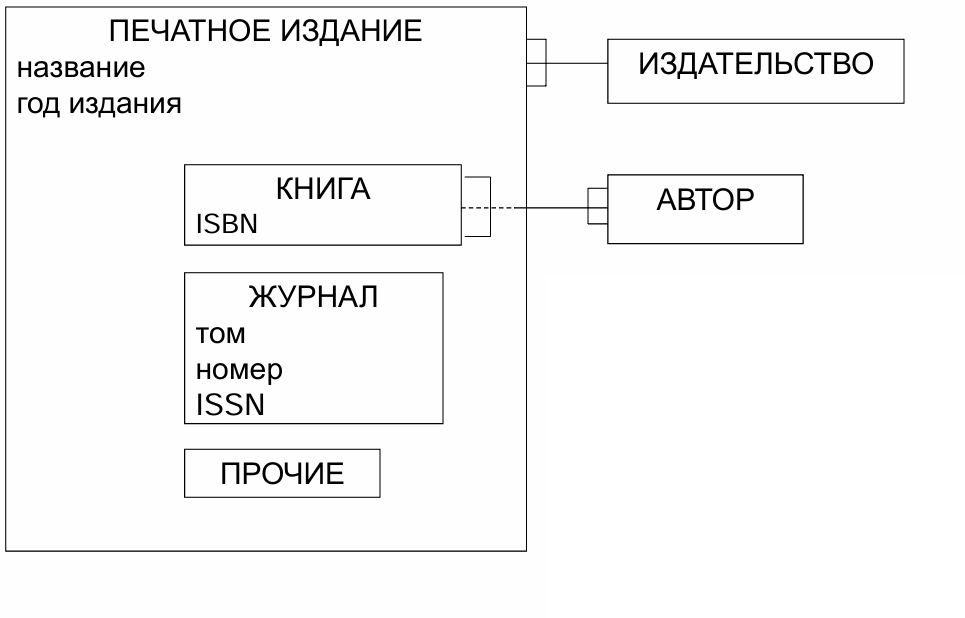
\includegraphics[width=0.75\linewidth]{image.png}
    
    \label{fig:enter-label}
\end{figure}

В супертипе ``Печатное издание'' определяются два атрибута (название издания и год издания) и обязательная связь ``один-ко-многим'' с типом сущности ``Издательство''. Эти атрибуты и связь наследуются всеми подтипами этого супертипа.

\subsubsection{Описание подтипов}

\paragraph{Подтип ``Книга''} Дополнительно определяется атрибут ISBN (International Standard Book Number) и связь ``многие-ко-многим'' с авторами. В совокупности у данной сущности имеются три атрибута (два унаследованных от супертипа) и две связи (одна унаследованная).

\paragraph{Подтип ``Журнал''} Дополнительно определяются три атрибута: том, номер и ISSN (International Standard Serial Number). Аналогично, еще два атрибута и связь унаследованы от супертипа ``Печатное издание''.

Поскольку супертип ``Печатное издание'' в ER-модели является абстрактным, для возможности описания печатных изданий, не являющихся книгами или журналами (брошюры, листовки и т.п.), определяется дополнительный подтип ``Прочие''.

Подтипизация может продолжаться на более низких уровнях (например, можно определить подтипы сущности ``Книга'' или ``Журнал''), но опыт использования ER-модели при проектировании баз данных показывает, что в большинстве случаев оказывается достаточно двух-трех уровней.

\section{Взаимно исключающие связи в ER-модели. Примеры. Отображение диаграммы со взаимно исключающими связями в реляционную схему}

\subsection{Взаимно исключающие связи}

\textbf{Взаимно исключающими связями} называется такой набор связей одной сущности с другими, что для каждого экземпляра сущности может или должен существовать экземпляр только одной связи из данного набора.

\subsubsection{Примеры взаимно исключающих связей}

\begin{itemize}
    \item \textbf{Самолет:} Самолет может быть исправным (тогда у него есть один пилот) или неисправным (тогда он ремонтируется авиаремонтным предприятием).
    \item \textbf{Банковский счет:} Банковский счет может принадлежать либо физическому, либо юридическому лицу.
\end{itemize}

\subsection{Преобразования диаграмм со взаимно исключающими связями}

\begin{enumerate}
    \item \textbf{Введение подтипов}
    
    \begin{center}
        \begin{tikzpicture}[node distance=2cm, auto]
            \node[entity] (airplane) {САМОЛЕТ};
            \node[entity] (pilot) [below left of=airplane] {ПИЛОТ};
            \node[entity] (repair) [below right of=airplane] {АРП НЕИСПРАВНЫЙ};
            \node[entity] (fixed) [below of=airplane, node distance=3cm] {ИСПРАВНЫЙ};
            
            \draw[relationship] (airplane) -- (pilot);
            \draw[relationship] (airplane) -- (repair);
            \draw[relationship] (airplane) -- (fixed);
        \end{tikzpicture}
    \end{center}
    
    \item \textbf{Введение общего супертипа}
    
    \begin{center}
        \begin{tikzpicture}[node distance=2cm, auto]
            \node[entity] (bankAccount) {БАНКОВСКИЙ СЧЕТ};
            \node[entity] (physPerson) [below left of=bankAccount] {ФИЗ. ЛИЦО};
            \node[entity] (jurPerson) [below right of=bankAccount] {ЮР. ЛИЦО};
            \node[entity] (owner) [below of=bankAccount, node distance=3cm] {ВЛАДЕЛЕЦ СЧЕТА};
            
            \draw[relationship] (bankAccount) -- (physPerson);
            \draw[relationship] (bankAccount) -- (jurPerson);
            \draw[relationship] (bankAccount) -- (owner);
        \end{tikzpicture}
    \end{center}
\end{enumerate}

\subsection{Уникальные идентификаторы экземпляров сущностей}

При определении сущности необходимо гарантировать, что каждый ее экземпляр является отличимым от любого другого экземпляра этой же сущности. Это достигается путем введения уникальных идентификаторов.

В ER-модели у экземпляра типа сущности не может быть назначаемого пользователем имени или назначаемого системой внешнего уникального идентификатора. Экземпляр сущности может идентифицироваться только своими индивидуальными характеристиками: значениями атрибутов и экземплярами связей.

Поэтому в качестве уникального идентификатора сущности проектировщик может выбрать (и сообщить об этом CASE-системе):
\begin{itemize}
    \item Атрибут
    \item Комбинацию атрибутов
    \item Связь
    \item Комбинацию связей
    \item Комбинацию атрибутов и связей
\end{itemize}

\subsubsection{Выбор уникального идентификатора экземпляров сущности «Человек»}

\begin{center}
    \begin{tabular}{|c|c|c|c|c|}
        \hline
        \textbf{ЧЕЛОВЕК} & фио & дата рождения & пол & \textbf{ИМЕЕТ} \\
        \hline
        \multicolumn{5}{|c|}{ПРИНАДЛЕЖИТ} \\
        \hline
        \textbf{ПАСПОРТ} & серия & номер & дата выдачи & кем выдан \\
        \hline
    \end{tabular}
\end{center}

\begin{itemize}
    \item \textbf{Для БД небольших предприятий:} либо фио, либо фио + дата рождения.
    \item \textbf{Для БД крупных предприятий, городов, регионов:} связь с паспортом, тогда в качестве УИД человека будет использоваться УИД его паспорта (серия + номер).
    \item \textbf{Замечание:} связь с человеком не может использоваться в качестве УИД паспорта, поскольку могут существовать еще не выданные людям бланки паспортов.
\end{itemize}

\subsubsection{Выбор уникального идентификатора экземпляров сущности «Книга»}

\begin{itemize}
    \item \textbf{Книжный склад:} прообразом типа сущности будет набор одноименных книг одного автора, вышедших в одном издательстве (уникально характеризуемый ISBN, который и является УИД). Дополнительно вводится атрибут, определяющий доступное количество экземпляров книг в этом наборе.
    
    \item \textbf{Библиотека:} требуется различать индивидуальные экземпляры книг (даже одинаковых), поэтому в каждой библиотеке экземплярам книг присваивается уникальный библиотечный номер, который и может использоваться в качестве УИД. ISBN в данном случае не уникален.
\end{itemize}

\subsubsection{Пример выбора уникального идентификатора для сущности «Курс»}

\begin{itemize}
    \item Профессора обладают знаниями в нескольких учебных дисциплинах.
    \item Преподавание каждой дисциплины доступно нескольким профессорам.
    \item Каждый профессор может готовить курсы по любой доступной ему дисциплине.
    \item По каждой дисциплине может преподаваться несколько учебных курсов.
    \item Но каждый курс должен готовиться только одним профессором и быть посвящен только одной дисциплине.
\end{itemize}

Таким образом, каждый экземпляр сущности ``Курс'' уникально идентифицируется парой связей с именами концов ``Готовится'' и ``Посвящен'' или же уникальными идентификаторами экземпляров соответствующих сущностей ``Профессор'' и ``Дисциплина''. Заметим, что сущности ``Профессор'' и ``Дисциплина'' связями не идентифицируются (соответствующие роли не являются уникальными).

\section{Диаграммы классов языка UML. Основные понятия. Отображение классов, стереотипов, комментариев и ограничений на диаграммах. Примеры.}

Диаграммой классов в UML называется диаграмма, на которой показан набор классов и некоторых других сущностей, а также связи между этими классами, и, возможно, комментарии и ограничения. Ограничения могут задаваться как на естественном языке, так и на языке объектных ограничений OCL.

\subsection{Класс}

Класс — это именованное описание совокупности объектов с общими атрибутами, операциями, связями и семантикой. Изображается в виде прямоугольника. У класса должно быть уникальное имя, которое рекомендуется сделать коротким, осмысленным и читаемым.

\subsubsection{Атрибут}

Атрибутом класса называется именованное свойство класса, описывающее множество значений, которые могут принимать экземпляры этого свойства. Атрибут является абстракцией состояния объекта. Класс может иметь любое число атрибутов. Любой атрибут должен иметь некоторое значение. Имена атрибута записываются под именем класса, и рекомендации для них такие же, как и для имени класса.

\subsubsection{Операция}

Операция класса — это именованная услуга, которую можно запросить у любого объекта этого класса. Класс может содержать любое число операций. Операции записываются под атрибутами и могут содержать сигнатуру и тип значения операции.

\subsection{Связи}

В диаграмме классов могут участвовать связи трех разных категорий: зависимости, обобщения и ассоциации.

\subsubsection{Зависимость}

Зависимость называется связью по применению, когда изменение в спецификации одного класса может повлиять на поведение другого класса, использующего первый. Изображается пунктирной линией со стрелкой, направленной к классу, от которого имеется зависимость.

Наиболее частое применение связей-зависимостей: при использовании стереотипа в качестве типа атрибута или в сигнатуре операции зависимого класса либо использование одного класса в сигнатуре операции другого класса.

\subsubsection{Обобщение}

Обобщением называется связь между общим классом (суперклассом) и более специализированной его разновидностью (подклассом). Подклассы могут использоваться везде, где могут использоваться суперклассы — это называется полиморфизм по включению. Связь обобщения изображается сплошной линией с большой незакрашенной стрелкой, направленной к суперклассу. Допускается множественное наследование, в котором есть ряд проблем, в том числе проблема именования атрибутов.

\subsubsection{Ассоциация}

Ассоциацией называется структурная связь между объектами одного класса и объектами другого или того же самого класса. В UML допускается создание n-арных ассоциаций, связывающих сразу несколько классов. Изображается как сплошная линия. Дополнительными параметрами ассоциации являются имя, роль каждого класса, участвующего в ассоциации, и кратность, показывающая, сколько объектов класса может участвовать в каждом экземпляре ассоциации.

Обычная ассоциация характеризует связь между равноправными классами. Если связь имеет вид часть-целое, то такая ассоциация называется агрегатной и изображается дополнительным ромбом на стороне класса-целого, закрашенным, если часть не может существовать без целого.

\subsection{Стереотипы}

Стереотип — механизм расширения семантики UML, позволяющий создавать новые элементы UML на основе существующих (например, классов) с учётом особенностей решаемой задачи.

\subsection{Комментарии и ограничения}

Комментарии и ограничения могут быть добавлены на диаграмму классов для уточнения дополнительных свойств или правил, которые должны соблюдаться при проектировании системы. Ограничения могут задаваться как на естественном языке, так и на языке объектных ограничений OCL.

\section{Диаграммы классов языка UML. Категории связей и их отображение на диаграмме. Примеры.}

Категории связей UML включают зависимости, обобщения и ассоциации.

\subsection{Зависимости}

Зависимостью называется связь по применению, когда изменение в спецификации одного класса может повлиять на поведение другого класса, использующего первый. Изображается пунктирной линией, направленной от зависимого класса.

Наиболее частое применение связей-зависимостей: использование стереотипа в качестве типа атрибута или в сигнатуре операции зависимого класса либо использование одного класса в сигнатуре операции другого класса.

При проектировании реляционных БД непонятно, как использовать информацию о наличии связей-зависимостей. При использовании диаграммы классов для генерации программного кода наличие связи-зависимости является сигналом для генерации директив \texttt{include} или \texttt{import} в исходном коде зависимого класса.

\subsection{Обобщения в UML}

Обобщением называется связь между общим классом (суперклассом) и более специализированной его разновидностью (подклассом). Класс-потомок наследует все атрибуты и операции класса-предка, но в нем могут быть определены дополнительные атрибуты и операции. Изображается сплошной линией с незакрашенным треугольником, направленным к суперклассу (родителю).

\subsubsection{Правила наследования в ER-модели (см. предыдущую лекцию)}

\begin{enumerate}
    \item \textbf{Включение}: $\forall b \in B_i \rightarrow b \in A, \quad i = 1, \ldots, n$ — выполняется в UML.
    \item \textbf{Отсутствие собственных экземпляров у супертипа}: $\forall a \in A \rightarrow a \in B_i, \quad i = 1, \ldots, n$ — не выполняется в UML по умолчанию (исключение: объявление суперкласса абстрактным, это внутреннее свойство класса, не отображаемое на диаграмме).
    \item \textbf{Разъединенность подтипов}: $\forall b \in B_i \rightarrow b \notin B_j, \quad i \neq j$ — не выполняется в UML по умолчанию (исключение: ограничение обобщения \{\texttt{disjoint}\}).
\end{enumerate}

\subsubsection{Пример с использованием связей обобщений UML}


\begin{figure}
    \centering
    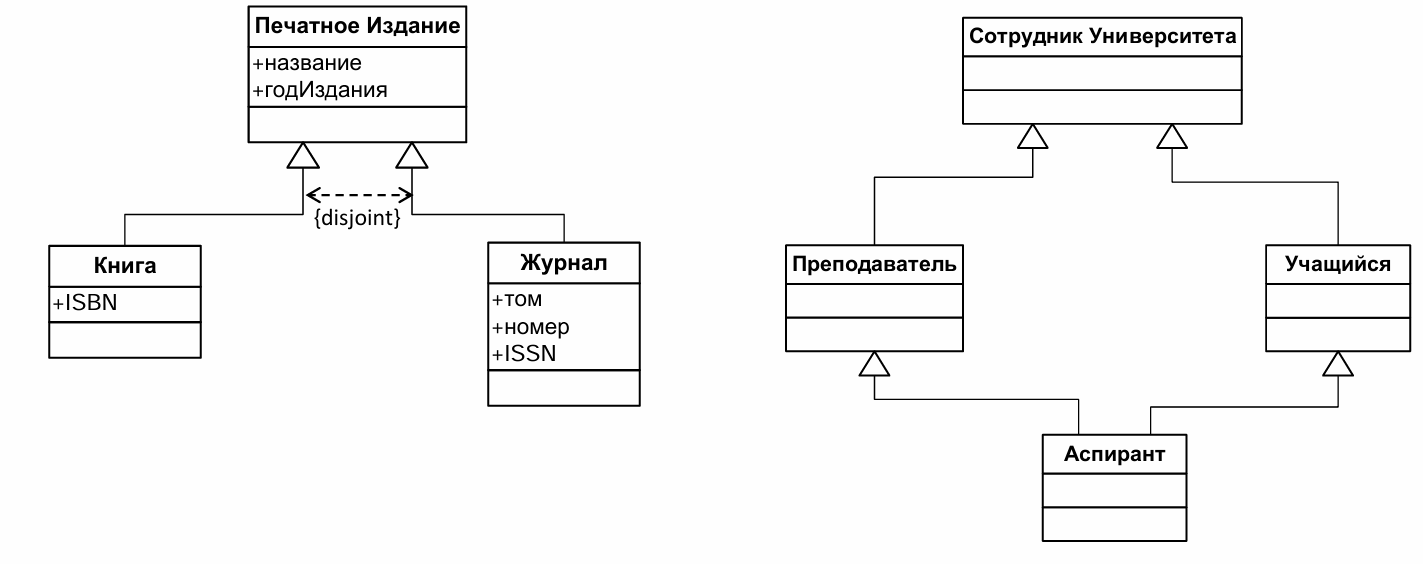
\includegraphics[width=0.75\linewidth]{image2.png}
    \caption{43.2.3}
    \label{fig:enter-label}
\end{figure}
Класс ``Прочие'' в UML не требуется, так как суперклассы по умолчанию не являются абстрактными и могут иметь собственные экземпляры.

\subsubsection{Проблемы использования множественного наследования}

Одиночное наследование является достаточным в большинстве случаев применения связи-обобщения в диаграмме классов, предназначенной для проектирования реляционной БД.

Множественное наследование, помимо того, что не слишком часто требуется на практике, порождает ряд проблем, из которых одной из наиболее известных является проблема именования атрибутов и операций в подклассе, полученном путем множественного наследования.

\begin{itemize}
    \item \textbf{Пример}: в классах ``Учащийся'' и ``Преподаватель'' может быть определён атрибут ``номерКомнаты'', где значениями этого атрибута будут номера комнат в студенческом общежитии для учащихся и номера служебных кабинетов для преподавателей. Аспирант может проживать в общежитии и при этом иметь рабочий кабинет, предоставленный кафедрой.
\end{itemize}

\subsection{Ассоциации в UML}

Ассоциацией называется структурная связь между объектами одного класса и объектами другого или того же самого класса. В UML допускается создание n-арных ассоциаций, связывающих сразу несколько классов. Изображается сплошной линией (в общем случае ненаправленной).
\subsection{Агрегатные ассоциации в UML}

Агрегатные ассоциации используются для отображения отношений ``часть-целое'', где класс ``целое'' имеет более высокий концептуальный уровень, чем часть. В агрегатных ассоциациях часть может одновременно принадлежать нескольким целым. Уничтожение целого не приводит к автоматическому уничтожению всех его частей.

\subsection{Навигация между ассоциированными объектами}
\begin{figure}
        \centering
        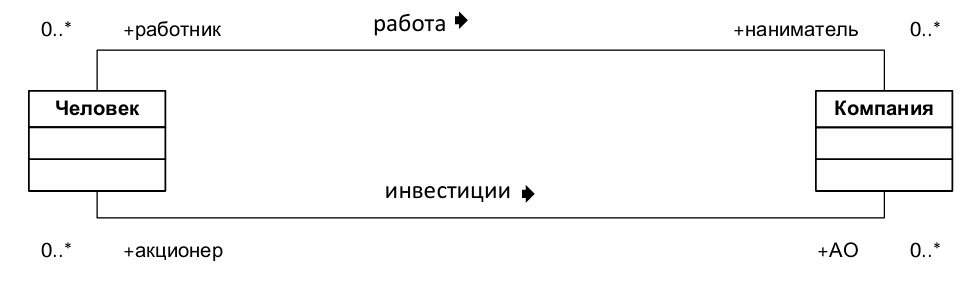
\includegraphics[width=1\linewidth]{image3.png}
        \caption{43.3}
        \label{fig:enter-label}
    \end{figure}

При наличии ассоциации предполагается возможность навигации между объектами, входящими в один экземпляр ассоциации. По умолчанию в UML навигация может проводиться в обоих направлениях. Для ограничения направления навигации на линии ассоциации ставится стрелка, указывающая требуемое направление.

\subsection{Взаимно исключающие связи в UML}

Для организации взаимно исключающих связей используется ограничение ассоциации \{\texttt{xor}\}.

\begin{center}
    \begin{figure}
        \centering
        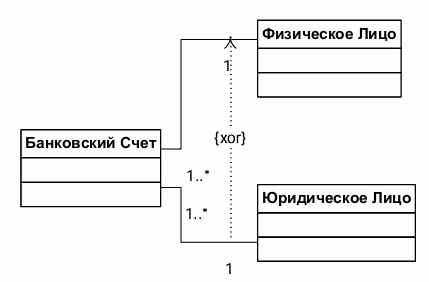
\includegraphics[width=0.5\linewidth]{image4.png}
        \caption{43.6 }
        \label{fig:enter-label}
    \end{figure}
\end{center}

\section{Язык OCL. Инварианты классов. Основные типы данных и выражения OCL.}

OCL — язык объектных ограничений, на котором могут быть написаны ограничения классов в диаграммах классов языка UML. Из UML в OCL заимствованы следующие понятия: класс, атрибут, операция, объект (экземпляр класса), ассоциация, тип данных, значение (экземпляр типа данных).

\subsection{Инварианты класса}

Под инвариантом класса в OCL понимается условие, которому должны удовлетворять все объекты данного класса при создании и в течение всего времени своего существования.

Синтаксис инварианта следующий:
\[
\text{context } <\text{class\_name}> \text{ inv: } <\text{OCL-выражение}>
\]
Где:
\begin{itemize}
    \item \textbf{<class\_name>} — имя класса, для которого определяется инвариант.
    \item \textbf{inv} — ключевое слово, указывающее, что определяется инвариант.
    \item \textbf{<OCL-выражение>} — логическое выражение, которое должно быть истинным для всех объектов данного класса.
\end{itemize}

\subsection{Типы данных OCL}

\subsubsection{Скалярные типы}
\begin{itemize}
    \item \textbf{Integer}
    \item \textbf{Real}
    \item \textbf{Boolean}
    \item \textbf{String}
\end{itemize}

\subsubsection{Коллекции}
\begin{itemize}
    \item \textbf{Set} — неупорядоченная коллекция, не содержащая одинаковых элементов.
    \item \textbf{Bag} — неупорядоченная коллекция, которая может содержать одинаковые элементы.
    \item \textbf{Sequence} — упорядоченная коллекция, которая может содержать одинаковые элементы.
    \item \textbf{OrderedSet} — упорядоченная коллекция, не содержащая одинаковых элементов.
\end{itemize}

\subsubsection{Объектные типы}
Классы, определённые в UML.

\subsection{Операции над значениями скалярных типов OCL}

\begin{itemize}
    \item \textbf{Boolean}: \texttt{and}, \texttt{or}, \texttt{xor}, \texttt{not}, \texttt{implies}, \texttt{if-then-else-endif}
    \item \textbf{Integer}: \texttt{*}, \texttt{+}, \texttt{-}, \texttt{/}, \texttt{abs()}, \texttt{div()}, \texttt{mod()}, \texttt{min()}, \texttt{max()}, операции сравнения
    \item \textbf{Real}: \texttt{*}, \texttt{+}, \texttt{-}, \texttt{/}, \texttt{abs()}, \texttt{floor()}, \texttt{round()}, \texttt{min()}, \texttt{max()}, операции сравнения
    \item \textbf{String}: \texttt{concat()}, \texttt{size()}, \texttt{substring()}, \texttt{toLower()}, \texttt{toUpper()}
\end{itemize}

\subsection{Операции над объектами}

\begin{itemize}
    \item \textbf{Получение значения атрибута}: \texttt{<объект>.<имя\_атрибута>}
    \item \textbf{Переход по экземпляру ассоциации}: \texttt{<объект>.<имя\_роли>}
    \item \textbf{Вызов операции класса}: \texttt{<объект>.<имя\_операции>(<список\_фактических\_параметров>)}
\end{itemize}

\subsection{Операции над коллекциями OCL}

\subsubsection{Конструкторы коллекций}

\begin{itemize}
    \item \textbf{select(<логическое выражение>)} — конструирует новую коллекцию, состоящую из тех элементов исходной коллекции, для которых результатом вычисления логического выражения является \texttt{true}.
    \item \textbf{reject(<логическое выражение>)} — конструирует новую коллекцию, состоящую из тех элементов исходной коллекции, для которых результатом вычисления логического выражения является \texttt{false}.
    \item \textbf{collect(<выражение>)} — конструирует новую коллекцию, состоящую из новых элементов, значения которых вычисляются путем применения заданного выражения к каждому элементу исходной коллекции.
\end{itemize}

\subsubsection{Кванторы}

\begin{itemize}
    \item \textbf{exists(<логическое выражение>)} — возвращает \texttt{true}, если результат вычисления заданного логического выражения равен \texttt{true} хотя бы для одного из элементов коллекции.
    \item \textbf{forAll(<логическое выражение>)} — возвращает \texttt{true}, если результат вычисления заданного логического выражения равен \texttt{true} для всех элементов коллекции.
\end{itemize}

\subsubsection{Теоретико-множественные операции}

\begin{itemize}
    \item \textbf{union(<коллекция>)} — конструирует новую коллекцию, включающую все элементы из исходной и заданной коллекций.
    \item \textbf{intersection(<коллекция>)} — конструирует новую коллекцию, включающую элементы, которые присутствуют одновременно как в исходной, так и в заданной коллекциях.
    \item \textbf{difference(<коллекция>)} — конструирует новую коллекцию, включающую те элементы исходной, которые отсутствуют в заданной коллекции.
    \item \textbf{symmetricDifference(<коллекция>)} — конструирует новую коллекцию, включающую элементы, которые присутствуют либо в исходной, либо в заданной коллекциях, но не в обеих из них.
\end{itemize}

\subsubsection{Прочие операции}

\begin{itemize}
    \item \textbf{count(<элемент>)} — возвращает число вхождений заданного элемента в коллекцию.
    \item \textbf{includes(<элемент>)} — возвращает \texttt{true}, если коллекция содержит заданный элемент.
    \item \textbf{excludes(<элемент>)} — возвращает \texttt{true}, если коллекция не содержит заданный элемент.
    \item \textbf{includesAll(<коллекция>)} — возвращает \texttt{true}, если исходная коллекция содержит все элементы заданной коллекции.
    \item \textbf{excludesAll(<коллекция>)} — возвращает \texttt{true}, если коллекция не содержит ни одного элемента заданной коллекции.
    \item \textbf{size()} — возвращает число элементов в коллекции.
    \item \textbf{at(<индекс>)} — возвращает значение элемента в заданной позиции, применимо к \texttt{sequence} и \texttt{orderedSet}.
    \item \textbf{min()}, \textbf{max()}, \textbf{sum()} — для коллекций чисел определяются минимальное, максимальное значения и сумма значений всех элементов соответственно.
\end{itemize}

\subsection{Инвариант класса}

Инвариант класса — логическое выражение, при вычислении которого для любого объекта данного класса должно получаться значение \texttt{true} в течение всего времени существования этого объекта.

\subsection{Пример инварианта класса}

\textbf{Класс} 
Студент \\
\textbf{Инвариант} \\
\texttt{self.стипендия>=Университет.minСтипендия и self.стипендия<=Университет.maxСтипендия} \\

\section{Получение реляционной схемы из диаграммы классов UML. Основные проблемы и рекомендации.}
Если не обращать внимания на различия в терминологии, то
здесь выполняются практически те же шаги, что и в случае
преобразования в схему реляционной БД ER-диаграммы
Поэтому ограничимся только некоторыми рекомендациями,
специфичными для диаграмм классов.
\\
\textbf{Рекомендация 1.}: Прежде чем определять в классах
операции, подумайте, что вы будете делать с этими
определениями в среде целевой РСУБД
Если в этой среде поддерживаются хранимые процедуры, то,
возможно, некоторые операции могут быть реализованы
именно с помощью такого механизма
Но если в среде РСУБД поддерживается механизм
определяемых пользователями функций, возможно, он
окажется более подходящим 
\\
\textbf{Рекомендация 2.}: Помните, что сравнительно
эффективно в РСУБД реализуются только
ассоциации видов «один ко многим» и «многие
ко многим»
Если в созданной диаграмме классов имеются
ассоциации «один к одному», следует задуматься о
целесообразности такого проектного решения
Реализация в среде РСУБД ассоциаций с точно
заданными кратностями ролей возможна, но требует
определения дополнительных триггеров, выполнение
которых понизит эффективность
\\
\textbf{Рекомендация 3.}: В спецификации UML говорится
о том, что, определяя однонаправленные связи,
вы можете способствовать эффективности
доступа к некоторым объектам
Для технологии реляционных баз данных поддержка
такого объявления вызовет дополнительные накладные
расходы и тем самым снизит эффективность
\\
\textbf{Рекомендация 4.}: Не злоупотребляйте
возможностями OCL.
\\
Диаграммы классов UML – это мощный
инструмент для создания концептуальных схем
баз данных, но, как известно, все хорошо в меру

\section{Язык баз данных SQL. Возможности и структура языка SQL. Основные черты модели данных SQL и ее отличия от реляционной модели. Критика SQL.}

Язык баз данных SQL  
Предложен: 1974 г., исследовательский проект IBM System R.  
Первоначальное название: \texttt{SEQUEL (Structured English QUEry Language)}.  
По юридическим соображениям в 1977 г. название языка было сокращено до \texttt{SQL (Structured Query Language)}.  
Еще одна интерпретация аббревиатуры \texttt{SQL}: \texttt{Standard Query Language}.  
Однако до сих пор многие произносят аббревиатуру \texttt{SQL} как “sequel”.  
Стандарт: ANSI (первая версия, 1986 г.), ISO (\texttt{ISO-9075})

Возможности языка SQL  
\begin{itemize}
\item Формулирование запросов к БД
\item Манипулирование данными (\texttt{CREATE}, \texttt{MODIFY}, \texttt{DELETE})
\item Определение и манипулирование схемой БД
\item Определение ограничений целостности данных
\item Определение представлений (виртуальных таблиц)
\item Определение структур физического уровня, поддерживающих эффективное исполнение запросов
\item Авторизация доступа к данным
\item Управление транзакциями, сессиями, подключениями
\end{itemize}

Структура языка SQL  
С точки зрения разработчиков СУБД  
\begin{itemize}
\item Базовый
\item Промежуточный
\item Полный
\end{itemize}

Базовый SQL – минимальное подмножество языка, реализация которого является обязательным условием соответствия стандарту.  
Промежуточный SQL – подмножество языка, реализация которого желательна в СУБД (именно этот уровень и поддерживается в большинстве реализаций).  
Полный SQL – реализация данного уровня является целью, к которой следует стремиться.

Критерий отнесения конструкции языка к определенному уровню – сложность ее реализации.

Структура языка SQL  
С точки зрения программиста приложений БД  
\begin{itemize}
\item Прямой
\item Встраиваемый
\item Динамический
\end{itemize}

Прямой SQL – конструкции языка, которые можно использовать при прямом взаимодействии пользователя с СУБД в интерактивном режиме (например, через консольное приложение).

Встраиваемый SQL – включает конструкции, которые позволяют использовать возможности прямого SQL в программах, написанных на традиционных языках программирования.

Динамический SQL – добавляются конструкции, которые позволяют приложениям обращаться к СУБД с использованием конструкций прямого SQL, динамически образуемыми во время выполнения программы.

Структура языка SQL  
\texttt{SQL}  
\texttt{DDL}  
\texttt{DML}  
\texttt{DQL}  
\texttt{(условное DAL)}

Разделение на подъязыки:  
\begin{itemize}
\item \texttt{Data Definition Language} – язык определения данных (определение схемы базы данных: таблиц, доменов, типов данных, ограничений целостности данных и т.п.)
\item \texttt{Data Manipulation Language} – язык манипулирования данными (создание, модификация, удаление данных)
\item \texttt{Data Query Language} – язык запросов (выборки данных)
\item \texttt{Data Administration Language (DCL)} – язык администрирования или язык управления: определение прав доступа к данным, управление транзакциями, сессиями, подключениями
\end{itemize}

Подразделение на подъязыки действительно является условным: конструкции одного подъязыка могут включать конструкции другого.

Наиболее известные реализации SQL-ориентированных СУБД  
SQL-ориентированные коммерческие СУБД:  
1979 г. \texttt{Oracle}  
1981 г. \texttt{IBM SQL/DS} на коде System R (до конца 90-х)  
1983 г. \texttt{IBM DB2}  
1985 г. \texttt{INFORMIX SQL} (в 2001 г. приобретена IBM, продукт продолжает поддерживаться IBM)  
1987 г. \texttt{Sybase SQL Server} (в 2010 г. компания Sybase приобретена SAP, SAP использует SQL Server в составе своих интегрированных решений, но не продает как отдельный продукт)  
1989 г. \texttt{Microsoft SQL Server} (по технологии Sybase)

Бесплатные дистрибутивы коммерческих СУБД  
\texttt{Oracle XE (Express Edition)}  
\texttt{IBM DB2 Community Edition}  
\texttt{Microsoft SQL Server Express (ограничения функционала)}

Наиболее известные реализации SQL-ориентированных СУБД  
Наиболее распространенные реализации с открытым кодом:  
1996 г. \texttt{PostgreSQL} (Berkley University, М. Стоунбрейкер, сообщество PostgreSQL)  
\begin{itemize}
\item Лицензия \texttt{PostgreSQL} позволяет на его основе создавать различные, в том числе коммерческие, ответвления
\item \texttt{Postgres Plus (EnterpriseDB)} – наиболее известный продукт с двойной лицензией (свободная без поддержки и коммерческая с официальной поддержкой)
\item \texttt{Postgres Pro (Postgres Professional, Россия)} – сертификат ФСТЭК для использования в государственных организациях
\end{itemize}

1998 г. \texttt{MySQL} (М. Видениус, MySQL AB, c 2008 г. Sun Microsystems, c 2010 г. принадлежит Oracle) – двойная лицензия: \texttt{GPL} и коммерческая  
2009 г. \texttt{MariaDB} (М. Видениус, MariaDB Foundation) – ответвление MySQL, лицензия \texttt{GPL}  
2000 г. \texttt{FirebirdSQL} (Firebird Foundation) – \texttt{Mozilla Public License}  
\begin{itemize}
\item 2007 г. \texttt{Ред База Данных (Ред Софт, Россия)}, свободная и коммерческая лицензия, сертификат ФСТЭК
\end{itemize}

Наиболее известные реализации SQL-ориентированных СУБД  
Все вышеперечисленные СУБД относятся к универсальным клиент-серверным СУБД  
Из файл-серверных SQL-ориентированных СУБД следует выделить \texttt{Informix Standard Engine (SE)}, которая в настоящее время не поддерживается, и \texttt{OpenOffice/LibreOffice Base}

Встраиваемые SQL-ориентированные СУБД:  
\begin{itemize}
\item \texttt{SQLite} – написан на C, исходный код передан автором (Р. Хипп) в общественное достояние
\item \texttt{HSQLDB} – написан на Java, входит в состав OpenOffice Base, лицензия BSD
\item \texttt{Firebird Embedded} – движок FirebirdSQL в одной библиотеке, написан на C++, входит в состав LibreOffice Base, лицензия MPL
\item \texttt{Microsoft SQL Server Compact Edition} (не выпускается с 2013 г.)
\end{itemize}

Стандартизация языка SQL  
\begin{tabular}{c|c|l}
Поколение & Год & Стандарт \& Изменения \\ \hline
1 & 1986 & SQL-86 Первоначальная версия \\ 
  & 1989 & SQL-89 Четкая стандартизация синтаксиса и семантики операторов выборки данных, манипулирования данными и определения ограничений целостности \\
2 & 1992 & SQL-92 Манипулирование схемой, транзакциями, сессиями, подключениями, динамический SQL \\
  & 1995 & SQL/CLI (Call-Level Interface) \\
  & 1996 & SQL/PSM (Persistent Stored Modules) \\
3 & 1999 & SQL:1999 ОО расширения, регулярные выражения, триггеры, рекурсивные запросы \\
  & 2003 & SQL:2003 Java, XML, поддержка OLAP \\
  & 2006 & Переработано один том: поддержка языка XQUERY для XML \\
  & 2008 & SQL:2008 Улучшена поддержка OLAP, XQUERY, расширение триггеров \\
  & 2011 & SQL:2011 Улучшена поддержка темпоральных данных \\
  & 2016 & SQL:2016 Работа с JSON, полиморфные табличные функции, поиск строк по шаблону \\
  & 2019 & Добавлен новый том: поддержка многомерных массивов \\
  & 2023 & SQL:2023 Тип данных JSON, работа с графами (Property Graph Queries)
\end{tabular}

Структура стандарта SQL (2003-2023)  
\begin{itemize}
\item Том 1: Framework – Концептуальная структура стандарта
\item Том 2: Foundation – Синтаксис, семантика, правила связывания для процедурных языков программирования
\item Том 3: Call-Level Interface – Интерфейс уровня вызовов (основа SQL-ориентированных API)
\item Том 4: Persistent Stored Modules – Описание языка SQL/PSM
\item Том 9: Management of External Data – Языковые средства взаимодействия с внешними данными
\item Том 10: Object Language Bindings – Правила связывания для объектно-ориентированных языков программирования
\item Том 11: Information and Definition Schemas – Описание информационной схемы (хранение описателей данных)
\item Том 13: SQL Routines and Types Using the Java Programming Language – Использование SQL совместно с языком программирования Java
\item Том 14: XML-Related Specifications – Языковые средства работы с XML документами
\item Том 15 (2019): Multi-dimensional Arrays – Поддержка работы с многомерными массивами
\item Том 16 (2023): Property Graph Queries – Мэппинг графов в SQL и язык запросов для доступа к графам, хранящимся в таблицах SQL (основан на GQL)
\end{itemize}

Отличие модели данных SQL от классической реляционной модели  
SQL-ориентированная база данных представляет собой набор таблиц, каждая из которых в любой момент времени содержит некоторое мультимножество строк, соответствующих заголовку таблицы. Заголовок таблицы представляет собой список столбцов таблицы: поддерживается порядок столбцов, соответствующий порядку их определения при создании таблицы (при изменении таблицы новые столбцы добавляются всегда в конец заголовка). Во временных таблицах, порождаемых запросами SQL, допускаются безымянные столбцы, а также дублирование имен столбцов.

\begin{enumerate}
\item Отношение РМД – множество кортежей; таблица SQL – мультимножество строк:
  \begin{itemize}
  \item В SQL допускаются дубликаты строк в таблицах
  \item Ограничение первичного ключа для таблицы SQL не является обязательным
  \end{itemize}
\item В РМД заголовок отношения – множество атрибутов; в SQL заголовок таблицы – список столбцов
\item В РМД \texttt{NULL} не является допустимым значением для атрибутов, составляющих первичный или возможный ключ отношения; в SQL это правило действует только для первичных ключей
\item В РМД существует единственный способ сопоставления внешнего ключа с первичным/возможным; в SQL таких способов три, только один из которых соответствует РМД
\item Разная терминология (\textbf{РМД} – отношение, атрибут, кортеж; \textbf{SQL} – таблица, столбец, строка); таблица SQL – это вовсе не отношение, хотя во многом они похожи
\end{enumerate}

Критика языка SQL  
\begin{enumerate}
\item Противоречие принципам реляционной модели данных
\item Сложность языка (противоречие первоначальной идее авторов сделать язык доступным для понимания не квалифицированными пользователями)
\item Чрезмерная избыточность языка (например, имеется несколько способов выразить один и тот же запрос)
\item Отступления от стандарта в реализациях (многочисленные диалекты SQL, особенно это касается языка SQL/PSM)
\item Трехзначная логика (\texttt{False}, \texttt{True}, \texttt{Unknown})
\item Неоднозначность использования и интерпретации \texttt{NULL}
\end{enumerate}

Значение \texttt{NULL} в SQL  
\begin{enumerate}
    \item Означает ``отсутствие значения'', но на самом деле используется в трех разных по смыслу ситуациях (т.е. требуется три различных \texttt{NULL}, но это приведет к усложнению логики):
    \begin{itemize}
        \item значение неизвестно;
        \item значение временно не определено;
        \item значение недопустимо в данном контексте.
    \end{itemize}
    
    \item Для логического типа \texttt{NULL} и \texttt{UNKNOWN} трактуются как одно и то же значение, хотя \texttt{NULL} — это ``отсутствие значения'', а \texttt{UNKNOWN} — вполне определенное логическое значение.
    
    \item По правилам SQL сравнение значения с \texttt{NULL} дает в результате \texttt{UNKNOWN} (\texttt{a comp\_op NULL = NULL comp\_op a = NULL comp\_op NULL = UNKNOWN}), но для операции равенства это не всегда так:
    \begin{itemize}
        \item Равенство как операция сравнения (\texttt{a = NULL}) = (\texttt{NULL = a}) = (\texttt{NULL = NULL}) = \texttt{UNKNOWN};
        \item Поиск дубликатов: (\texttt{NULL = NULL}) = \texttt{TRUE}, (\texttt{a = NULL}) = (\texttt{NULL = a}) = \texttt{FALSE}.
    \end{itemize}
\end{enumerate}

\section{Основные типы данных языка SQL (без учета объектных расширений). Преобразования типов данных.}

Типы данных SQL  
\begin{itemize}
    \item Данные, хранящиеся в таблицах SQL, являются типизированными.
    \item СУБД должна отслеживать, чтобы в каждом столбце каждой строки таблицы присутствовали только допустимые для соответствующих типов данных значения.
    \item \texttt{NULL} является допустимым значением для любого типа данных SQL.
\end{itemize}

Булевский тип:  
\texttt{BOOLEAN}  
Литералы: \texttt{FALSE}, \texttt{TRUE}, \texttt{UNKNOWN}  
\texttt{SQL:2003}: ``В этой спецификации не проводится различие между \texttt{NULL} значением булевского типа данных и истинностным значением \texttt{UNKNOWN}, являющимся результатом вычисления предиката, условия поиска или булевского выражения. Они могут использоваться взаимозаменяемо и означают в точности одно и то же''.

Точные числовые типы  
Целые числа: \texttt{SMALLINT}, \texttt{INTEGER}, \texttt{BIGINT}  
Точность представления определяется в реализации, стандарт лишь определяет, что точность \texttt{SMALLINT $\leq$ INTEGER $\leq$ BIGINT}.

Литералы: десятичные целые числа со знаками \texttt{‘+’} или \texttt{‘-’}, отсутствие знака – \texttt{‘+’}.

Числа с фиксированной точкой:  
\texttt{NUMERIC(p, s)}, \texttt{DECIMAL(p, s)}  
\texttt{p} – точность (число сохраняемых десятичных цифр, включая дробную часть): максимально допустимая для \texttt{NUMERIC}, минимальная для \texttt{DECIMAL} (пример: литерал \texttt{123.4} недопустим для \texttt{NUMERIC(3,1)}, но допустим для \texttt{DECIMAL(3,1)}).  
\texttt{s} – масштаб (число десятичных цифр в дробной части).  
Допустимые значения \texttt{p}, \texttt{s} определяются в реализации (\texttt{p $\geq$ s}).  
Значения по умолчанию: \texttt{s=0}, \texttt{p} – определяется в реализации.

Литералы: целые или вещественные числа в формате с фиксированной точкой (точка отделяет целую часть от дробной), со знаком или без.  
В большинстве реализаций \texttt{NUMERIC} и \texttt{DECIMAL} трактуются как один и тот же тип.

Приближенные числовые типы  
\texttt{REAL}, \texttt{DOUBLE PRECISION}, \texttt{FLOAT(p)}  
\texttt{p} – число бит, требуемых для хранения мантиссы (точность представления).  
Точность представления для первых двух типов и максимальное значение \texttt{p} определяется в реализации.  
Литералы: целые числа, или вещественные числа в формате с фиксированной точкой, или вещественные числа в формате с плавающей точкой: \texttt{xEy}, где \texttt{x} – мантисса, \texttt{y} – десятичный порядок в виде целого числа (\texttt{x $\times$ 10$^y$}).  
Арифметика для приближенных числовых типов работает быстрее, чем для чисел с фиксированной точкой, но возможна потеря точности за счет погрешности вычислений.  
Числа с фиксированной точностью надо использовать там, где требуется соблюдать точность вычисления (финансы).

Типы символьных и битовых строк  
\texttt{CHAR(x)}, \texttt{VARCHAR(x)}, \texttt{CLOB(z)}  
\texttt{x, z} – количество символов в строке: фиксированное для \texttt{CHAR} (допустимо записывать литералы меньшей длины, которые будут дополняться справа пробелами), максимально допустимое для \texttt{VARCHAR} и \texttt{CLOB}.  
Допустимые значения \texttt{x, z} определяются в реализации (\texttt{z} значительно больше \texttt{x}), \texttt{z} может указываться в виде \texttt{nK}, \texttt{nM}, \texttt{nG}.  
Вид литералов: \texttt{‘abCdef’} или \texttt{``FbcDE''}.  
Набор допустимых символов определяется в реализации (\texttt{ASCII} как минимум).

\texttt{BIT(x)}, \texttt{BIT VARYING(x)}, \texttt{BLOB(z)}  
В отличие от строк состоят из произвольных байтов, не обязательно кодирующих символы.  
Вид литералов: \texttt{B'01001101101'} или \texttt{X'79CA83'}.

Типы даты, времени  
\texttt{DATE}, \texttt{TIME(p)}, \texttt{TIMESTAMP(p)}, \texttt{TIME WITH TIMEZONE(p)}, \texttt{TIMESTAMP WITH TIMEZONE(p)}  
\texttt{p} – точность представления долей секунды, максимальное значение определяется в реализации (\texttt{p $\geq$ 6}), значение по умолчанию \texttt{p=0} для \texttt{TIME}, \texttt{p=6} для \texttt{TIMESTAMP}.  
Допустимое значение секунд варьируется от \texttt{00} до \texttt{61}.

Форматы литералов:  
\texttt{DATE 'yyyy-mm-dd'},  
\texttt{TIME 'hh:mm:ss:ff...f'},  
\texttt{TIMESTAMP 'yyyy-mm-dd hh:mm:ss:ff...f'}.  
Временная зона задается в виде \texttt{+hh:mm} или \texttt{-hh:mm}.

Функции, возвращающие текущие дату и время:  
\texttt{CURRENT\_DATE}, \texttt{CURRENT\_TIME}, \texttt{CURRENT\_TIMESTAMP}.

Типы временных интервалов  
\texttt{INTERVAL start(p) [TO end(q)]}  
\texttt{start, end}: \texttt{YEAR}, \texttt{MONTH}, \texttt{DAY}, \texttt{HOUR}, \texttt{MINUTE}, \texttt{SECOND}.  
Поддерживаемые интервалы:  
\begin{itemize}
    \item \texttt{YEAR}, \texttt{YEAR TO MONTH}, \texttt{MONTH}
    \item \texttt{DAY}, \texttt{DAY TO HOUR}, \texttt{DAY TO MINUTE}, \texttt{DAY TO SECOND}
    \item \texttt{HOUR}, \texttt{HOUR TO MINUTE}, \texttt{HOUR TO SECOND}
    \item \texttt{MINUTE}, \texttt{MINUTE TO SECOND}, \texttt{SECOND}
\end{itemize}

\texttt{p} – точность представления лидирующего поля, \texttt{q} – точность долей секунды (применяется, если \texttt{end=SECOND}), максимальные значения определяются в реализации, значения по умолчанию \texttt{p=2}, \texttt{q=6}.  
Формат литералов: \texttt{INTERVAL '1:35' HOUR TO MINUTE}.

Преобразование типов данных в SQL  
\begin{itemize}
    \item Поддерживается явное и неявное преобразование значений одного типа данных к другому.
    \item Правила неявного преобразования не сильно отличаются от тех, что существуют в языках программирования.
    \item Точный числовой тип приводится к другому точному числовому типу с большей точностью или к приближенному числовому типу.
    \item Приближенный числовой тип приводится к другому приближенному числовому типу с большей точностью.
    \item Строковый тип фиксированной длины приводится к другому строковому типу фиксированной или переменной длины с большим допустимым количеством символов.
    \item Строковый тип переменной длины приводится к другому строковому типу переменной длины с большим допустимым количеством символов.
    \item Явное преобразование осуществляется с помощью оператора \texttt{CAST(expression AS datatype)}.
    \item Подробные правила выполнения оператора \texttt{CAST} см. в учебной литературе.
\end{itemize}

\section{Средства работы с доменами в SQL.}

Домены в SQL  \\
Домен – базовый тип данных + ограничение области определения значений \\  
Домен является долговременно хранимым именованным объектом схемы БД  \\
Оператор определения домена:  
\texttt{CREATE DOMAIN domain\_name AS datatype [DEFAULT value] [constraint\_list]}  
\texttt{DEFAULT value} – определение значения по умолчанию (литерал базового типа, либо значение \texttt{NULL}, либо вызов предопределенной функции, возвращающей литеральное значение базового типа)  
\texttt{constraint\_list} – список ограничений области определения значений, все ограничения в списке связываются логической функцией \texttt{AND}

Пример:  \\
\texttt{CREATE DOMAIN SALARY AS NUMERIC(10, 2) \\
DEFAULT 10000.00 \\
CHECK( VALUE BETWEEN 10000.00 AND 10000000.00 ) \\
CONSTRAINT SAL\_NOT\_NULL CHECK( VALUE IS NOT NULL );}

Домены в SQL  \\
Оператор изменения определения домена:  \\
\texttt{ALTER DOMAIN domain\_name action}  
Допустимы 4 действия:  \\
\texttt{SET DEFAULT value}, \texttt{DROP DEFAULT}, \texttt{ADD CONSTRAINT [constraint\_name] constraint\_expression}, \texttt{DROP CONSTRAINT constraint\_name}  
Если к моменту исполнения \texttt{ALTER DOMAIN ADD CONSTRAINT} существуют столбцы таблиц, определенные на данном домене, текущие значения которых противоречат новому ограничению, то СУБД должна отвергнуть этот оператор.  
Новое ограничение связывается с существующими ограничениями домена логической функцией \texttt{AND}.

Пример:  
\texttt{ALTER DOMAIN SALARY SET DEFAULT 20000.00;}  
\texttt{ALTER DOMAIN SALARY DROP CONSTRAINT SAL\_NOT\_NULL;}

Домены в SQL  
Оператор отмены определения домена:  
\texttt{DROP DOMAIN domain\_name \{ RESTRICT | CASCADE \}}  
\texttt{DROP DOMAIN RESTRICT} отвергается, если домен использован в определении некоторого столбца таблицы (базовой или виртуальной) или в определении ограничения целостности.  
\texttt{DROP DOMAIN CASCADE} выполняется всегда по следующим правилам:
\begin{itemize}
    \item Уничтожаются все ограничения целостности и виртуальные таблицы, в определениях которых задействован данный домен
    \item Столбцы базовых таблиц, определенные на данном домене, преобразуются к его базовому типу и наследуют значение по умолчанию и все ограничения уничтожаемого домена
\end{itemize}

\section{Средства определения, изменения и отмены определения базовых таблиц в SQL}

Таблицы в SQL  
\begin{itemize}
    \item Базовые – реально хранимые в БД таблицы (подразделяются на традиционные и типизированные)
    \item Порождаемые – таблицы, формируемые и существующие во время выполнения запросов
    \item Представления (виртуальные) – таблицы, существование которых поддерживается алгоритмически
\end{itemize}

Оператор определения базовой (традиционной) таблицы:  
\begin{lstlisting}
CREATE TABLE table_name (
    column_list [constraint_list]
)
column_definition ::= column_name { datatype | domain } [DEFAULT value] [constraint_list]
\end{lstlisting}

Данный оператор создает соответствующие описатели в схеме БД и выделяет область во внешней памяти для хранения данных.

Изменение определения базовой таблицы  
\begin{lstlisting}
ALTER TABLE table_name action
\end{lstlisting}

Возможны следующие действия:  
\begin{itemize}
    \item \texttt{ADD COLUMN column\_name \{ datatype | domain \} [DEFAULT value] [constraint\_list]}
    \item \texttt{ALTER COLUMN column\_name SET DEFAULT value}
    \item \texttt{ALTER COLUMN column\_name DROP DEFAULT}
    \item \texttt{DROP COLUMN column\_name \{ RESTRICT | CASCADE \}}
    \item \texttt{ADD CONSTRAINT [constraint\_name] constraint\_expression}
    \item \texttt{DROP CONSTRAINT constraint\_name [ \{ RESTRICT | CASCADE \} ]}
\end{itemize}

Отмена определения базовой таблицы  
\begin{lstlisting}
DROP TABLE table_name { RESTRICT | CASCADE }
\end{lstlisting}

\texttt{DROP TABLE RESTRICT} отвергается, если таблица задействована в определении представлений или ограничений целостности (не считая собственных табличных ограничений, не ссылающихся на другие базовые таблицы).

\texttt{DROP TABLE CASCADE} выполняется всегда по следующим правилам:
\begin{itemize}
    \item Уничтожаются все ограничения целостности и представления, в определениях которых задействована данная таблица.
    \item Уничтожаются все строки, хранящиеся в данной таблице, а также определения ее столбцов и табличных ограничений (таблица перестает существовать).
\end{itemize}


\section{Иерархия ограничений в SQL. Средства определения и отмены общих ограничений (ограничений БД).}

Иерархия ограничений целостности языка SQL:
\begin{itemize}
    \item Ограничения БД
    \item Ограничения таблиц
    \item Ограничения столбцов
    \item Ограничения доменов
\end{itemize}

Дополнительные ограничения базы данных – общие ограничения целостности

Определение:
\begin{lstlisting}
CREATE ASSERTION constraint_name
CHECK( constraint_expression )
\end{lstlisting}

Отмена:
\begin{lstlisting}
DROP ASSERTION constraint_name
\end{lstlisting}

Пример:
\begin{lstlisting}
CREATE ASSERTION DEPT_MNG_CONSTR
CHECK( NOT EXISTS(
    SELECT * FROM EMPLOYEE EMP, DEPARTMENT DEPT
    WHERE EMP.EMP_ID = DEPT.DEPT_MANAGER
      AND CURRENT_DATE - EMP.EMP_BDATE < INTERVAL '30' YEAR
));
\end{lstlisting}

\section{Базовые средства манипулирования данными в языке SQL}

Базовые средства манипулирования данными  
\begin{itemize}
    \item Средства манипулирования данными присутствуют в прямом, встраиваемом и динамическом SQL
    \item К базовым средствам манипулирования данными относятся:
    \begin{itemize}
        \item Оператор вставки строк (\texttt{INSERT})
        \item Оператор модификации строк (\texttt{UPDATE})
        \item Оператор удаления строк (\texttt{DELETE})
    \end{itemize}
\end{itemize}

Оператор вставки строк  
\begin{lstlisting}
INSERT INTO table_name [(column_list)] VALUES row_constructor_list
\end{lstlisting}

\begin{itemize}
    \item Если список столбцов пропущен, то предполагается, что используется список из имен всех столбцов таблицы, указанных в том порядке, в котором они были описаны в операторе \texttt{CREATE TABLE}
    \item В списке столбцов должны быть обязательно указаны те столбцы, для которых не задано значение по умолчанию (явно или неявно)
    \item Порядок перечисления значений столбцов в конструкторе строки должен совпадать с порядком перечисления столбцов в соответствующем списке
    \item В качестве значений столбцов могут использоваться литералы, \texttt{DEFAULT}, \texttt{NULL}, вызовы предопределенных функций, возвращающих литеральное значение соответствующего типа, а также скалярные запросы, результат выполнения которых состоит из единственной строки, включающей единственный столбец
\end{itemize}

Пример:
\begin{lstlisting}
INSERT INTO EMPLOYEE VALUES  
ROW( 319, 'Ivanov I.I.', '1980-07-19', DEFAULT, NULL, NULL ),  
ROW( 320, 'Petrov P.P.', '1983-05-09', (SELECT EMP_SALARY FROM EMPLOYEE WHERE EMP_ID = 200), 12, NULL );
\end{lstlisting}


\begin{lstlisting}
INSERT INTO EMPLOYEE( EMP_ID, EMP_NAME, EMP_BDATE ) VALUES  
ROW(321, 'Sidorov S.S.', '1962-12-10' );
\end{lstlisting}

Оператор вставки строк – вставка результата запроса  
Определим таблицу, хранящую информацию о временных сотрудниках:
\begin{lstlisting}
CREATE TABLE EMPLOYEE_TEMP (
    EMPT_ID INTEGER PRIMARY KEY,
    EMPT_NAME VARCHAR(200) NOT NULL,
    EMPT_BDATE DATE NOT NULL,
    EMPT_ENTRY_DATE DATE NOT NULL
);
\end{lstlisting}

Переведем временных сотрудников, чей испытательный срок превысил 3 месяца, в основной штат:
\begin{lstlisting}
INSERT INTO EMPLOYEE( EMP_ID, EMP_NAME, EMP_BDATE )
( SELECT EMPT_ID, EMPT_NAME, EMPT_BDATE FROM EMPLOYEE_TEMP
  WHERE CURRENT_DATE - EMPT_ENTRY_DATE >= INTERVAL '3' MONTH );
\end{lstlisting}

Оператор модификации строк  
\begin{lstlisting}
UPDATE table_name SET column_value_assignment_list WHERE logical_expression
column_value_assignment := column_name = value_expression
\end{lstlisting}

\begin{itemize}
    \item Для всех строк таблицы с указанным именем вычисляется логическое условие. Строки, для которых значением этого условия является \texttt{TRUE}, считаются подлежащими модификации (\texttt{S\_m} – множество модифицируемых строк)
    \item Каждая строка \texttt{s ∈ S\_m} подвергается модификации таким образом, что значение каждого столбца этой строки, указанного в списке модификации, заменяется значением, указанным в правой части соответствующего элемента списка. Если новое значение задается оператором запроса, в который входят имена модифицируемых столбцов, то под значениями этих столбцов в запросе понимаются их значения до модификации
\end{itemize}

Пример. Перевести всех служащих, выполняющих проект с номером 5, в отдел 12 и повысить им заработную плату на 5000 руб.
\begin{lstlisting}
UPDATE EMPLOYEE SET DEPT_ID = 12, EMP_SALARY = EMP_SALARY + 5000.00 WHERE PRO_ID = 5;
\end{lstlisting}

Оператор удаления строк  
\begin{lstlisting}
DELETE FROM table_name WHERE logical_expression
\end{lstlisting}

\begin{itemize}
    \item Для всех строк таблицы с указанным именем вычисляется логическое условие. Строки, для которых значением этого условия является \texttt{TRUE}, считаются подлежащими удалению (\texttt{S\_d} – множество удаляемых строк)
    \item Каждая строка \texttt{s ∈ S\_d} удаляется из указанной таблицы.
\end{itemize}

Пример. Уволить всех служащих, размер заработной платы которых превышает размер заработной платы начальников их отделов.
\begin{lstlisting}
DELETE FROM EMPLOYEE WHERE EMP_SALARY >  
(SELECT EMP.EMP_SALARY  
 FROM EMPLOYEE EMP, DEPARTMENT DEPT  
 WHERE EMPLOYEE.DEPT_ID = DEPT.DEPT_ID  
   AND DEPT.DEPT_MANAGER = EMP.EMP_ID);
\end{lstlisting}

Учебный пример
\begin{lstlisting}
CREATE TABLE EMPLOYEE (
    ...
    DEPT_ID INTEGER DEFAULT NULL REFERENCES DEPARTMENT ON DELETE SET NULL,
    ...
);
CREATE TABLE DEPARTMENT (
    DEPT_ID INTEGER PRIMARY KEY,
    DEPT_EMP_NUM INTEGER NOT NULL CHECK ( DEPT_EMP_NUM = ( SELECT COUNT(*) FROM EMPLOYEE WHERE DEPT_ID = EMPLOYEE.DEPT_ID )),
    CHECK( VALUE <= 100 ),
    ...
);
\end{lstlisting}

Операторы модификации таблицы \texttt{EMPLOYEE} вида:
\begin{lstlisting}
INSERT INTO EMPLOYEE ( ..., DEPT_ID, ...) VALUES ROW ( ..., X, ...);
UPDATE EMPLOYEE SET DEPT_ID = X WHERE ...;
DELETE FROM EMPLOYEE WHERE ...;
\end{lstlisting}

где \texttt{X} – значение \texttt{DEPT\_ID}, отличное от \texttt{NULL}, а во множество удаляемых строк включается хотя бы одна строка, в которой значение столбца \texttt{DEPT\_ID} отличается от \texttt{NULL}, нарушают выделенное ограничение целостности.

\section{Понятие триггера. Механизм триггеров в SQL. Типы триггеров и их выполнение.}

Триггеры в SQL\\
Триггер – хранимая в БД процедура, автоматически вызываемая СУБД при возникновении определенных условий. В языке обеспечиваются возможности определения триггеров, которые вызываются при модификации указанной базовой таблицы (определение триггеров над представлениями не допускается).

\textbf{Предметная таблица} – базовая таблица, с которой связывается определение триггера.\\
\textbf{Инициирующий оператор} – оператор SQL, выполнение которого приводит к срабатыванию триггера.

Основные области применения триггеров:
\begin{itemize}
    \item Согласование и очистка данных
    \item Журнализация и аудит
    \item Операции, не связанные с изменением БД (генерация отчетов, печать документов, рассылка почты)
\end{itemize}

\subsection{Определение триггера}

Оператор \texttt{CREATE TRIGGER} (отмена – \texttt{DROP TRIGGER}). В операторе указываются:
\begin{enumerate}
    \item Имя триггера
    \item Момент срабатывания: \texttt{BEFORE} или \texttt{AFTER}
    \item Тип инициирующего оператора: \texttt{INSERT}, \texttt{UPDATE [OF column\_list]} или \texttt{DELETE}
    \item Имя предметной таблицы: \texttt{ON table\_name [REFERENCING OLD \{ROW | TABLE\} AS name NEW \{ROW | TABLE\} AS name]}
    \item Количество срабатываний триггера: \texttt{FOR EACH ROW} или \texttt{FOR EACH STATEMENT}
    \item Дополнительное условие применимости триггера: \texttt{WHEN (logical\_expression)}
    \item Тело триггера: одиночный оператор или процедура на языке \texttt{SQL/PSM}
\end{enumerate}

\subsection{Триггеры для учебного примера}

\begin{lstlisting}
CREATE TRIGGER CHANGE_DEPT_I AFTER INSERT ON EMPLOYEE FOR EACH ROW
WHEN( EMPLOYEE.DEPT_ID IS NOT NULL )
UPDATE DEPARTMENT SET DEPT_EMP_NUM = DEPT_EMP_NUM + 1 WHERE DEPARTMENT.DEPT_ID = EMPLOYEE.DEPT_ID;
\end{lstlisting}

\begin{lstlisting}
CREATE TRIGGER CHANGE_DEPT_D AFTER DELETE ON EMPLOYEE FOR EACH ROW
WHEN( EMPLOYEE.DEPT_ID IS NOT NULL )
UPDATE DEPARTMENT SET DEPT_EMP_NUM = DEPT_EMP_NUM - 1 WHERE DEPARTMENT.DEPT_ID = EMPLOYEE.DEPT_ID;
\end{lstlisting}

\begin{lstlisting}
CREATE TRIGGER CHANGE_DEPT_U AFTER UPDATE OF DEPT_ID ON EMPLOYEE
REFERENCING OLD ROW AS OLD_EMP NEW ROW AS NEW_EMP FOR EACH ROW
BEGIN ATOMIC
    UPDATE DEPARTMENT SET DEPT_EMP_NUM = DEPT_EMP_NUM - 1 WHERE DEPARTMENT.DEPT_ID = OLD_EMP.DEPT_ID;
    UPDATE DEPARTMENT SET DEPT_EMP_NUM = DEPT_EMP_NUM + 1 WHERE DEPARTMENT.DEPT_ID = NEW_EMP.DEPT_ID;
END;
\end{lstlisting}

\subsection{Выполнение триггеров}

При выполнении каждого триггера система устанавливает контекст выполнения триггера. Контекст выполнения триггера всегда является атомарным. Контекст выполнения триггера включает:
\begin{itemize}
    \item триггерное событие (\texttt{INSERT}, \texttt{UPDATE} или \texttt{DELETE})
    \item имя предметной таблицы триггера
    \item имена столбцов предметной таблицы, специфицированных в определении триггера (для триггеров по \texttt{UPDATE})
    \item набор переходов (представление всех вставляемых, модифицируемых или удаляемых строк, а также список уже выполненных триггеров и представлений строк, над которыми эти триггеры выполнялись)
\end{itemize}

Отслеживание уже выполненных триггеров ведется для предотвращения зацикливания выполнения системы триггеров.

\section{Общая структура оператора выборки в SQL и схема его выполнения.}

Оператор выборки данных в SQL  
\begin{lstlisting}
SELECT [ ALL | DISTINCT ] select_item_list
FROM table_reference_list
[ WHERE logical_expression ]
[ GROUP BY column_name_list ]
[ HAVING logical_expression ]
[ ORDER BY order_item_list ]
\end{lstlisting}

Выполнение запроса состоит из нескольких шагов, соответствующих разделам оператора выборки.  
СУБД обычно не придерживаются данной схемы выполнения, но результат должен получиться таким, как если бы он получался при точном следовании данной схеме.

\subsection{Семантика оператора выборки}

\paragraph{Шаг 1: \texttt{FROM table\_reference\_list}}  
Выполняется операция расширенного декартова произведения таблиц, указанных в списке \texttt{FROM}: \texttt{T = T1 TIMES T2 TIMES … TIMES Tn}  
Аналогом операции переименования \texttt{RENAME} алгебры Кодда в SQL служат псевдонимы таблиц (пример: \texttt{EMPLOYEE E}) и квалифицированные имена столбцов (\texttt{E.EMP\_BDATE}).

\paragraph{Шаг 2: \texttt{[ WHERE logical\_expression ]}}  
Выполняется операция ограничения таблицы \texttt{T}, сформированной на предыдущем шаге, по заданному логическому условию: \texttt{T1 = T WHERE logical\_expression}  
\texttt{T1} содержит только те строки таблицы \texttt{T}, для которых результатом вычисления логического выражения является \texttt{TRUE}. Отсутствие \texttt{WHERE} означает \texttt{WHERE TRUE} (\texttt{T1 $\equiv$ T}).

\paragraph{Шаг 3: \texttt{[ GROUP BY column\_name\_list ]}}  
На основе таблицы \texttt{T1}, полученной на предыдущем шаге, формируется сгруппированная таблица \texttt{T2}.

\paragraph{Шаг 4: \texttt{[ HAVING logical\_expression ]}}  
Строится таблица \texttt{T3}, содержащая только те группы строк таблицы \texttt{T2}, для которых результатом вычисления логического выражения является \texttt{TRUE}.  
Отсутствие \texttt{HAVING} означает \texttt{HAVING TRUE} (\texttt{T3 $\equiv$ T2}).

\paragraph{Шаг 5: \texttt{SELECT [ ALL | DISTINCT ] select\_item\_list}}  
Результирующая таблица \texttt{T4} содержит столько строк, сколько \texttt{T1} (без группировки) или сколько групп \texttt{T3} (с группировкой).  
\texttt{DISTINCT} – на завершающей стадии из \texttt{T4} удаляются строки-дубликаты.

\paragraph{Шаг 6: \texttt{[ ORDER BY order\_item\_list ]}}  
На завершающей стадии выполнения выборки данных производится сортировка строк результирующей таблицы. \texttt{ORDER BY} не приводит к появлению таблицы, а к появлению упорядоченного списка строк.

Конструкция \texttt{TABLE table\_name} является сокращенной формой \texttt{SELECT * FROM table\_name}.

\subsection{Ссылки на таблицы раздела \texttt{FROM}}

\begin{itemize}
    \item Имя базовой таблицы (\texttt{CREATE TABLE})
    \item Имя представления (\texttt{CREATE VIEW})
    \item Порождаемая таблица (выражение запроса в круглых скобках)
    \item Имя запроса, присоединенного с помощью \texttt{WITH}
\end{itemize}

\subsection{Представления (виртуальные таблицы)}

\paragraph{Определение представления:}  
\texttt{CREATE VIEW view\_name [column\_name\_list] AS query\_expression}  
Явное указание имен столбцов представляемой таблицы требуется, если их невозможно вывести из выражения запроса.

\paragraph{Пример: создать представление с данными о начальниках отделов}  
\begin{lstlisting}
CREATE VIEW DEPARTMENT_MANAGER AS
SELECT E.EMP_ID, E.EMP_NAME, E.EMP_BDATE, E.EMP_SALARY, D.DEPT_ID, D.DEPT_NAME
FROM EMPLOYEE E, DEPARTMENT D WHERE E.EMP_ID = D.DEPT_MANAGER;
\end{lstlisting}

\paragraph{Отмена представления:}  
\texttt{DROP VIEW view\_name \{ RESTRICT | CASCADE \}}

Из представлений можно выполнять \texttt{SELECT}. В общем случае они не модифицируемы (без рассмотрения \texttt{WITH CHECK OPTION}).

\section{Представляемые и порождаемые таблицы в SQL. Агрегатные и кванторные функции.}

\textbf{Порождаемые таблицы и присоединенные запросы}\\
 Семантически порождаемые таблицы соответствуют временным 
представлениям, которые существуют лишь в момент исполнения запроса. 
Явное указание псевдонима порождаемой таблицы и имен ее столбцов 
требуется в том случае, когда эти имена невозможно вывести из 
соответствующего выражения запроса
Пример (Найти общее число служащих и максимальный размер зарплаты в 
отделах с одинаковым максимальным размером зарплаты.):
\begin{lstlisting}
WITH DEPT_MAX_SAL(MAX_SAL, TOTAL_EMP) AS
(
    SELECT MAX(EMP_SALARY), COUNT(*)
    FROM EMPLOYEE
    WHERE DEPT_ID IS NOT NULL
    GROUP BY DEPT_ID
)
SELECT SUM(TOTAL_EMP), MAX_SAL 
FROM DEPT_MAX_SAL 
GROUP BY MAX_SAL;
\end{lstlisting}

Агрегатные и кванторные функции

\texttt{Function( [ DISTINCT | ALL ] value\_expression )}
 \\Исходное мультимножество строк – вся таблица или группа строк в случае 
сгруппированной таблицы. На основании аргумента-выражения производится 
мультимножество значений путем вычисления данного выражения для 
каждой строки в мультимножестве. Из мультимножества значений удаляются 
NULL, а при наличии DISTINCT – и дубликаты. Затем производится вычисление.
\begin{itemize}
    \item \texttt{COUNT} - число строк (если аргумент *) или значений, 0 для пустого множества,
    
\item \texttt{MAX} –максимальное значение, NULL для пустого множества, \item\texttt{MIN} –минимальное значение, NULL для пустого множества, \item\texttt{AVG} –среднее значение, NULL для пустого множества, \item\texttt{SUM} –суммарное значение, NULL для пустого множества, \item\texttt{EVERY} – квантор всеобщности (TRUE, если вычисление аргумента равно TRUE 
для каждой строки исходного мультимножества, TRUE для пустого множества), \item\texttt{SOME/ANY} –квантор существования (TRUE, если вычисление аргумента 
равно TRUE хотя бы для одной строки исходного мультимножества, FALSE для
 пустого множества).
  \itemВажный частный случай: \texttt{COUNT(*)} – подсчет строк в мультимножестве (при 
этом все строки считаются различными)
\end{itemize}


\section{Предикаты в логических выражениях языка SQL}

Логические выражения в языке SQL\\
Синтаксически логическое выражение SQL определяется как булевское выражение, которое строится на основе предикатов с использованием логических операций \texttt{AND}, \texttt{OR} и \texttt{NOT}, а также круглых скобок.\\
В дальнейшем будем использовать следующие обозначения:
\begin{itemize}
    \item $s$ – скалярная величина
    \item $R$ – строковое значение
    \item $|R|$– степень строки (количество скалярных значений в ней)
    \item $T$– табличное значение
    \item $|T|$ - количество строк в таблице
\end{itemize}

Для предикатов выполняются следующие правила:
\begin{enumerate}
    \item Совместимость типов операндов
    \item Равенство степеней строк-операндов ($|RX| = |RY|$ или $|RX| = |RT|$, $RT \in T$)
    \item Существование отрицательной формы предиката: \texttt{NOT pred = NOT(pred)} – имеются исключения из данного правила
\end{enumerate}

\subsection{Предикат сравнения и предикат \texttt{BETWEEN}}

\textbf{Предикат сравнения}:\\
$s_X$ \texttt{op} $s_Y$ или $R_X$ \texttt{op} $R_Y$\\
\texttt{op} ::= = | <> | < | > | <= | >=\\
NULL \texttt{op} $s$ = UNKNOWN, $s$ \texttt{op} NULL = UNKNOWN, NULL \texttt{op} NULL = UNKNOWN

\textbf{Предикат \texttt{BETWEEN} (проверка вхождения в диапазон значений):}\\
$s_X$ \texttt{BETWEEN} $s_Y$ \texttt{AND} $s_Z$ или $R_X$ \texttt{BETWEEN} $R_Y$ \texttt{AND} $R_Z$, $|R_X| = |R_Y| = |R_Z|$\\
\textbf{Эквивалентные формы (выражение через предикаты сравнения):}\\
$s_X \geq s_Y$ \texttt{AND} $s_X \leq s_Z$ или $R_X \geq R_Y$ \texttt{AND} $R_X \leq R_Z$

\textbf{Пример:}\\
Найти номера, имена и размер зарплаты служащих, получающих зарплату, размер которой не меньше средней зарплаты служащих своего отдела и не больше зарплаты начальника отдела:
\begin{lstlisting}
SELECT E1.EMP_ID, E1.EMP_NAME, E1.EMP_SALARY 
FROM EMPLOYEE E1 
WHERE E1.EMP_SALARY BETWEEN 
    (SELECT AVG(E2.EMP_SALARY) 
     FROM EMPLOYEE E2 
     WHERE E2.DEPT_ID = E1.DEPT_ID) 
    AND 
    (SELECT MNG.EMP_SALARY 
     FROM DEPARTMENT_MANAGER MNG 
     WHERE MNG.DEPT_ID = E1.DEPT_ID);
\end{lstlisting}

\subsection{Предикат сравнения с квантором}

Квантифицированное сравнение строчного значения с табличным запросом:

\[
\begin{aligned}
\texttt{FALSE} &\leftrightarrow \exists RT \in T: (R_X \texttt{ op } RT) = \texttt{FALSE} \\
R_X \texttt{ op } \texttt{ALL } T &= \texttt{TRUE} \leftrightarrow \forall RT \in T \Rightarrow (R_X \texttt{ op } RT) = \texttt{TRUE} \lor T \equiv \emptyset \\
\texttt{UNKNOWN} &\leftrightarrow \forall RT \in T \Rightarrow (R_X \texttt{ op } RT) \neq \texttt{FALSE} \land \exists RT \in T: (R_X \texttt{ op } RT) = \texttt{UNKNOWN} \\
\texttt{TRUE} &\leftrightarrow \exists RT \in T: (R_X \texttt{ op } RT) = \texttt{TRUE} \\
R_X \texttt{ op } \texttt{SOME } T &= \texttt{FALSE} \leftrightarrow \forall RT \in T \Rightarrow (R_X \texttt{ op } RT) = \texttt{FALSE} \lor T \equiv \emptyset \\
\texttt{UNKNOWN} &\leftrightarrow \forall RT \in T \Rightarrow (R_X \texttt{ op } RT) \neq \texttt{TRUE} \land \exists RT \in T: (R_X \texttt{ op } RT) = \texttt{UNKNOWN} \\
R_X \texttt{ op } \texttt{ANY } T &\equiv R_X \texttt{ op } \texttt{SOME } T
\end{aligned}
\]

\textbf{Пример:}\\
Найти номера сотрудников отдела 12, зарплата которых в этом отделе не является минимальной:
\begin{lstlisting}
SELECT EMP_ID 
FROM EMPLOYEE 
WHERE DEPT_ID = 12 
  AND EMP_SALARY > 
    SOME (
        SELECT E1.EMP_SALARY 
        FROM EMPLOYEE E1 
        WHERE EMPLOYEE.DEPT_ID = E1.DEPT_ID
    );
\end{lstlisting}

\subsection{Предикат \texttt{IS NULL}}

Проверяет, являются ли неопределенными значения всех элементов строки операнда: \texttt{RX IS NULL}.

\[
\begin{array}{ll}
\texttt{RX IS NULL} & \texttt{RX IS NOT NULL} \\
|RX|=1, s=\texttt{NULL} & \texttt{TRUE} & \texttt{FALSE} & \texttt{FALSE} & \texttt{TRUE} \\
|RX|=1, s$\neq$\texttt{NULL} & \texttt{FALSE} & \texttt{TRUE} & \texttt{TRUE} & \texttt{FALSE} \\
|RX|>1, $\forall s \in RX \Rightarrow s=\texttt{NULL}$ & \texttt{TRUE} & \texttt{FALSE} & \texttt{FALSE} & \texttt{TRUE} \\
|RX|>1, $\forall i \neq j \exists s_i \in RX : s_i=\texttt{NULL} \land \exists s_j \in RX : s_j \neq \texttt{NULL}$ & \texttt{FALSE} & \texttt{FALSE} & \texttt{TRUE} & \texttt{TRUE} \\
|RX|>1, $\forall s \in RX \Rightarrow s \neq \texttt{NULL}$ & \texttt{FALSE} & \texttt{TRUE} & \texttt{TRUE} & \texttt{FALSE} \\
\end{array}
\]

\textbf{Пример:}\\
Найти номера и имена служащих, не задействованных в проектах:
\begin{lstlisting}
SELECT EMP_ID, EMP_NAME 
FROM EMPLOYEE 
WHERE PRO_ID IS NULL
\end{lstlisting}

\subsection{Предикат \texttt{IN}}

Проверяет факт вхождения скалярного значения или строки в указанное множество: \texttt{s IN (s1, s2, …, sn)} или \texttt{RX IN T}

\[
\begin{aligned}
\texttt{TRUE} &\leftrightarrow \exists RT \in T: (RX = RT) = \texttt{TRUE} \\
RX \texttt{ IN } T &= 
\begin{cases}
\texttt{FALSE} &\leftrightarrow \forall RT \in T \Rightarrow (RX = RT) = \texttt{FALSE} \lor T \equiv \emptyset \\
\texttt{UNKNOWN} &\leftrightarrow \forall RT \in T \Rightarrow (RX = RT) \neq \texttt{TRUE} \land \exists RT \in T: (RX = RT) = \texttt{UNKNOWN}
\end{cases}
\end{aligned}
\]

\textbf{Пример:}\\
Найти номера сотрудников, не являющихся начальниками отделов и получающих зарплату, размер которой равен размеру зарплаты какого-либо начальника отдела:
\begin{lstlisting}
SELECT EMP_ID 
FROM EMPLOYEE 
WHERE EMP_ID NOT IN (
    SELECT DEPT_MANAGER 
    FROM DEPARTMENT
) 
AND EMP_SALARY IN (
    SELECT EMP_SALARY 
    FROM DEPARTMENT_MANAGER
);
\end{lstlisting}

\subsection{Предикаты \texttt{LIKE} и \texttt{SIMILAR}}

Сопоставление символьных и битовых строк с заданным шаблоном:
\texttt{source\_string LIKE pattern\_string [ESCAPE symbol]}

В шаблоне могут использоваться два специальных символа:
\begin{itemize}
    \item \texttt{\_} (подчеркивание) – интерпретируется как произвольный одиночный символ
    \item \texttt{\%} (процент) – интерпретируется как произвольная подстрока произвольной длины
\end{itemize}

Для битовых строк используются коды соответствующих символов (X'5F' и X'25').

Раздел \texttt{ESCAPE} специфицирует одиночный символ (например, '\textbackslash'), используемый для изменения способа интерпретации '\_' и '\%'. Пары символов '\textbackslash\_' и '\textbackslash\%' будут интерпретироваться как одиночные символы '\_' и '\%' соответственно.

Основное отличие \texttt{SIMILAR} от \texttt{LIKE} состоит в возможности использования регулярных выражений внутри шаблона (в курсе лекций не рассматривается).

\textbf{Пример:}\\
Подсчитать количество проектов, в названии которых присутствует слово ‘software’:
\begin{lstlisting}
SELECT COUNT(*) 
FROM PROJECT 
WHERE PRO_TITLE LIKE '%software%' 
   OR PRO_TITLE LIKE '%Software%';
\end{lstlisting}

\subsection{Предикат \texttt{OVERLAPS}}

Служит для проверки перекрытия по времени двух событий: \texttt{RX OVERLAPS RY}, $|RX|=|RY|=2$, строки задаются в виде: (tS, tF) или (tS, \texttt{interval}), где tF = tS + \texttt{interval}

\textbf{Эквивалентное представление в виде предикатов сравнения:}
\[
\begin{aligned}
& ( t_{SX} = t_{SY} ) \lor \\
& ( t_{SX} > t_{SY} ) \land ( t_{SX} \leq t_{FY} \lor t_{FX} \leq t_{FY} ) \lor \\
& ( t_{SY} > t_{SX} ) \land ( t_{SY} \leq t_{FX} \lor t_{FY} \leq t_{FX} )
\end{aligned}
\]

\textbf{Пример:}\\
Найти названия проектов, которые будут выполняться в организации в одно и то же время:
\begin{lstlisting}
SELECT P1.PRO_ID, P2.PRO_ID 
FROM PROJECT P1, PROJECT P2 
WHERE P1.PRO_ID <> P2.PRO_ID 
  AND NOT (
    (P1.PRO_SDATE, P1.PRO_DURATION) IS DISTINCT FROM 
    (P2.PRO_SDATE, P2.PRO_DURATION)
  );
\end{lstlisting}

\subsection{Предикат \texttt{EXISTS}}

Проверяет наличие строк в результате запроса:

\[
\begin{aligned}
\texttt{TRUE} &\leftrightarrow |T| > 0 \\
\texttt{EXISTS}(T) &= \texttt{FALSE} \leftrightarrow |T| = 0
\end{aligned}
\]

Запросы с предикатом \texttt{EXISTS} можно переформулировать в виде запросов с предикатом сравнения и агрегатной функцией \texttt{COUNT(*)}.

\textbf{Пример:}\\
Найти номера отделов, среди служащих которых есть руководители проектов:
\begin{lstlisting}
SELECT D.DEPT_ID 
FROM DEPARTMENT D 
WHERE EXISTS (
    SELECT E.EMP_ID 
    FROM EMPLOYEE E 
    WHERE E.DEPT_ID = D.DEPT_ID 
      AND EXISTS (
          SELECT P.PRO_MANAGER 
          FROM PROJECT P 
          WHERE P.PRO_MANAGER = E.EMP_ID
      )
);
\end{lstlisting}

\subsection{Предикат \texttt{IS DISTINCT FROM}}

Позволяет проверить, являются ли две строки дубликатами.

\[
\texttt{RX IS DISTINCT FROM RY} = 
\begin{cases}
\texttt{FALSE} &\leftrightarrow \forall i=1, |RX| \Rightarrow (s_{Xi} = s_{Yi}) = \texttt{TRUE} \lor s_{Xi} = \texttt{NULL} \land s_{Yi} = \texttt{NULL},\ s_{Xi} \in RX,\ s_{Yi} \in RY \\
\texttt{TRUE} &\leftrightarrow \exists i: (s_{Xi} = s_{Yi}) = \texttt{FALSE} \lor s_{Xi} = \texttt{NULL} \land s_{Yi} \neq \texttt{NULL} \lor s_{Xi} \neq \texttt{NULL} \land s_{Yi} = \texttt{NULL}
\end{cases}
\]

Отрицательная форма предиката (\texttt{IS NOT DISTINCT FROM}) в языке SQL отсутствует.

\textbf{Пример:}\\
Найти пары номеров проектов, выполняющихся в организации в одно и то же время:
\begin{lstlisting}
SELECT P1.PRO_ID, P2.PRO_ID 
FROM PROJECT P1, PROJECT P2 
WHERE P1.PRO_ID <> P2.PRO_ID 
  AND NOT (
    (P1.PRO_SDATE, P1.PRO_DURATION) IS DISTINCT FROM 
    (P2.PRO_SDATE, P2.PRO_DURATION)
  );
\end{lstlisting}

\subsection{Предикат \texttt{UNIQUE}}

Служит для проверки факта отсутствия строк-дубликатов в результате запроса.

\[
\texttt{UNIQUE}(T) = \texttt{TRUE} \text{ тогда и только тогда, когда в таблице } T \text{ отсутствуют строки-дубликаты, в противном случае возвращается } \texttt{FALSE}.
\]

\textbf{Пример:}\\
Найти названия отделов, служащих которых можно различить по размеру получаемой зарплаты:
\begin{lstlisting}
SELECT DEPT_NAME 
FROM DEPARTMENT 
WHERE UNIQUE( SELECT EMP_SALARY 
              FROM EMPLOYEE 
              WHERE EMPLOYEE.DEPT_ID = DEPARTMENT.DEPT_ID );
\end{lstlisting}

\subsection{Предикат \texttt{MATCH}}

Условие соответствия строчного значения результату подзапроса:

\[
RX \texttt{ MATCH } [\texttt{UNIQUE}] \texttt{ SIMPLE } T = \texttt{TRUE} \leftrightarrow \exists s \in RX : s = \texttt{NULL} \lor \exists RT \in T : (RX = RT) = \texttt{TRUE}
\]

\[
RX \texttt{ MATCH } [\texttt{UNIQUE}] \texttt{ PARTIAL } T = \texttt{TRUE} \leftrightarrow \forall s \in RX \Rightarrow s = \texttt{NULL} \lor \exists RT \in T : \forall s_i \neq \texttt{NULL} \Rightarrow (s_i = s_{Ti}) = \texttt{TRUE},\ s_i \in RX,\ s_{Ti} \in RT
\]

\[
RX \texttt{ MATCH } [\texttt{UNIQUE}] \texttt{ FULL } T = \texttt{TRUE} \leftrightarrow \forall s \in RX \Rightarrow s = \texttt{NULL} \lor \forall s \in RX \Rightarrow s \neq \texttt{NULL} \land \exists RT \in T : (RX = RT) = \texttt{TRUE}
\]

Если указано \texttt{UNIQUE}, то дополнительно проверяется, является ли найденная строка RT уникальной в T (\texttt{FALSE}, если неуникальная).

\textbf{Пример:}\\
Найти номера служащих, зачисленных в один из отделов, для которых в их отделах работают служащие с той же самой датой рождения:
\begin{lstlisting}
SELECT EMP_ID 
FROM EMPLOYEE 
WHERE ( DEPT_ID, EMP_BDATE ) MATCH FULL (
    SELECT E1.DEPT_ID, E1.EMP_BDATE 
    FROM EMPLOYEE E1 
    WHERE E1.EMP_ID <> EMPLOYEE.EMP_ID
);
\end{lstlisting}



\section{Поддержка авторизации доступа к данным в SQL. Объекты и привилегии. Пользователи и роли.}

Метод авторизации доступа, используемый в SQL, относится к мандатным видам защиты данных: с каждым зарегистрированным в СУБД пользователем или ролью (субъектом) и каждым защищаемым объектом БД связывается мандат (или привилегия), определяющий действия, которые может выполнять данный субъект над данным объектом.

\textbf{Принцип сокрытия информации}: В SQL поддерживается принцип сокрытия информации об объектах, содержащихся в схеме БД, от субъектов, которые лишены доступа к этим объектам. Если некоторый субъект не обладает привилегиями доступа к некоторой таблице, то при попытке выполнить какое-либо действие над ней он получит такое же диагностическое сообщение, как если бы данная таблица не существовала.

\textbf{Владельцы объектов}: Создатель объекта базы данных автоматически становится владельцем этого объекта, который обладает полным набором привилегий для выполнения действий над объектом, в том числе привилегией на передачу всех или части своих привилегий другим субъектам.

\subsection{Привилегии доступа к объектам}

\begin{table}[h!]
    \centering
    \begin{tabular}{|l|l|l|}
        \hline
        \textbf{Действие} & \textbf{Привилегия} & \textbf{Объекты} \\
        \hline
        Просмотр & SELECT & Таблицы, столбцы, хранимые процедуры \\
        \hline
        Вставка & INSERT & Таблицы, столбцы \\
        \hline
        Модификация & UPDATE & Таблицы, столбцы \\
        \hline
        Удаление & DELETE & Таблицы \\
        \hline
        Ссылка & REFERENCES & Таблицы, столбцы \\
        \hline
        Использование & USAGE & Домены, типы и прочие определения \\
        \hline
        Инициирование & TRIGGER & Таблицы \\
        \hline
        Выполнение & EXECUTE & Хранимые процедуры \\
        \hline
        Типизация & UNDER & Определяемые пользователем типы \\
        \hline
        Передача & GRANT/ADMIN & Привилегии/роли \\
        \hline
    \end{tabular}
    \caption{Привилегии доступа к объектам}
\end{table}

Привилегии над представлениями основываются на привилегиях по отношению к базовым таблицам данных представлений.

\subsection{Пользователи и роли}

Привилегии доступа к объектам предоставляются пользователям, а также ролям, выполнение которых, в свою очередь, может предоставляться пользователям или другим ролям. С каждым пользователем и каждой ролью связывается уникальный идентификатор авторизации (\texttt{authID}).

\textbf{Роль}: Динамически образуемая группа пользователей СУБД, каждый из которых обладает привилегией на исполнение данной роли, а также всеми привилегиями данной роли для доступа к объектам БД. Роли упрощают построение и администрирование системы авторизации доступа.

В стандарте SQL не определяются средства создания и ликвидации идентификаторов пользователей. Для создания и ликвидации ролей поддерживаются операторы \texttt{CREATE ROLE}/\texttt{DROP ROLE}. В стандарте также поддерживается концепция идентификатора псевдопользователя \texttt{PUBLIC}, который соответствует любому пользователю, зарегистрированному в СУБД.

Пользователю \texttt{PUBLIC} могут предоставляться привилегии доступа к объектам базы данных, как и любому другому пользователю, при этом они будут распространяться автоматически и на всех вновь создаваемых пользователей.


\section{Передача и аннулирование привилегий и ролей в SQL.}
\subsection{Создание и ликвидация роли}

\subsubsection{Создание роли}

\textbf{Синтаксис:}
\begin{verbatim}
CREATE ROLE role_name [ WITH ADMIN { CURRENT_USER | CURRENT_ROLE } ]
\end{verbatim}

Имя роли должно отличаться от любого идентификатора авторизации (\texttt{authID}), уже определенного в СУБД. При наличии раздела \texttt{WITH ADMIN} привилегию на исполнение данной роли вместе с правом передачи привилегии получает либо текущий пользователь, либо текущая роль SQL сессии. По умолчанию привилегия на исполнение создаваемой роли передается текущему пользователю. Если SQL сессия не имеет пользователя, то текущей роли. Привилегии, требуемые для выполнения \texttt{CREATE ROLE}, определяются в реализациях (как правило, выполнение разрешается только администраторам).

\subsubsection{Ликвидация роли}

\textbf{Синтаксис:}
\begin{verbatim}
DROP ROLE role_name
\end{verbatim}

Для выполнения \texttt{DROP ROLE} текущий \texttt{authID} SQL сессии (пользователь или роль) должен являться владельцем данной роли. При ликвидации роли автоматически ликвидируются привилегии на ее исполнение у всех пользователей и ролей, которым эта привилегия ранее передавалась.

\subsection{Передача привилегий}

\textbf{Синтаксис:}
\begin{verbatim}
GRANT { ALL PRIVILEGES | privilege_list } ON object_name TO { PUBLIC | authID_list }
    [ WITH GRANT OPTION ]
    [ GRANTED BY { CURRENT_USER | CURRENT_ROLE } ]
\end{verbatim}

Привилегии передаются от текущего \texttt{authID} сессии (пользователя или роли) к указанным в списке \texttt{authID} (пользователям или ролям). Для этого он должен обладать привилегией на передачу всех или части привилегий из списка, указанного в операторе \texttt{GRANT}.

Если текущий \texttt{authID} обладает правом на передачу только части привилегий из этого списка, то передается именно эта часть и выдается предупреждение, а если он не имеет прав на передачу ни одной из перечисленных привилегий, то фиксируется ошибка.

Если указан раздел \texttt{WITH GRANT OPTION}, то привилегии из списка передаются с правом дальнейшей передачи.

Раздел \texttt{GRANTED BY} позволяет явно указать, от какого \texttt{authID} (текущего пользователя или текущей роли) передаются привилегии.

Избыточная дублирующая передача привилегий от имени одного и того же \texttt{authID} (authID1) другому (тому же самому) \texttt{authID} (authID2) игнорируется (при этом дублирующая передача привилегии с правом передачи и без права передачи независимо от порядка действий будет означать, что \texttt{authID2} обладает данной привилегией вместе с правом ее дальнейшей передачи).

\subsection{Передача ролей}

\textbf{Синтаксис:}
\begin{verbatim}
GRANT role_name_list TO { PUBLIC | authID_list }
    [ WITH ADMIN OPTION ]
    [ GRANTED BY { CURRENT_USER | CURRENT_ROLE } ]
\end{verbatim}

Оператор позволяет передавать произвольное число ролей произвольному числу пользователей или ролей.

Если текущий \texttt{authID} обладает правом на передачу только части ролей из этого списка, то передается именно эта часть и выдается предупреждение, а если он не имеет прав на передачу ни одной из перечисленных ролей, то фиксируется ошибка.

Если указан раздел \texttt{WITH ADMIN OPTION}, то привилегии на исполнение ролей из списка передаются с правом дальнейшей передачи.

Раздел \texttt{GRANTED BY} позволяет явно указать, от какого \texttt{authID} (текущего пользователя или текущей роли) передаются привилегии на исполнение ролей.

\subsection{Аннулирование привилегий}

\textbf{Синтаксис:}
\begin{verbatim}
REVOKE [ GRANT OPTION FOR ] privilege_list ON object_name FROM { PUBLIC | authID_list }
    [ GRANTED BY { CURRENT_USER | CURRENT_ROLE } ]
    { RESTRICT | CASCADE }
\end{verbatim}

\begin{itemize}
    \item \texttt{RESTRICT} – действие оператора отвергается, если хотя бы одна из указанных в списке привилегий была передана другому \texttt{authID}, у которого привилегия должна быть аннулирована.
    \item \texttt{CASCADE} – указанные привилегии аннулируются у всех \texttt{authID}, прямо или косвенно (через промежуточные \texttt{authID}) получивших привилегии от текущего \texttt{authID}, выполняющего данную операцию.
\end{itemize}

При наличии \texttt{GRANT OPTION FOR} аннулируется привилегия на передачу привилегий из указанного списка, сами привилегии при этом остаются, но при каскадном аннулировании отзыв привилегии на передачу у какого-либо \texttt{authID} означает и аннулирование самих привилегий у всех \texttt{authID}, прямо или косвенно получивших ее от данного \texttt{authID}.

Для успешного выполнения \texttt{REVOKE} необходимо, чтобы текущий \texttt{authID} обладал всеми или частью привилегий из указанного списка. В последнем случае аннулируется именно эта часть (с выдачей предупреждения).

Если текущий \texttt{authID} не обладает привилегиями на передачу ни одной из перечисленных привилегий, операция \texttt{REVOKE} завершится ошибкой.

\subsection{Аннулирование ролей}

\textbf{Синтаксис:}
\begin{verbatim}
REVOKE [ ADMIN OPTION FOR ] role_name_list FROM { PUBLIC | authID_list }
    [ GRANTED BY { CURRENT_USER | CURRENT_ROLE } ]
    { RESTRICT | CASCADE }
\end{verbatim}

Действие операции аннулирования ролей очень похоже на действие операции аннулирования привилегий. Отличия состоят в том, что аннулируются не привилегии, а роли, а также в том, что для аннулирования привилегии на передачу роли используется раздел \texttt{ADMIN OPTION FOR}.

Если некоторая привилегия или роль была передана \texttt{PUBLIC}, то ей обладают все пользователи. Но нет возможности аннулировать такую привилегию или роль у отдельно указываемого пользователя. Привилегия или роль была передана всем, и аннулировать ее можно только сразу у всех, то есть у псевдопользователя \texttt{PUBLIC}.

\section{Транзакции. Свойства ACID. Инициация и завершение транзакций в SQL. Проверка ограничений целостности и ее связь с механизмом транзакций. Точки сохранения.}

Поддержка механизма транзакций – показатель уровня развитости СУБД.

Корректное поддержание транзакций является основой обеспечения целостности баз данных, поэтому транзакции вполне уместны и в однопользовательских персональных СУБД.

Транзакции составляют базис изолированности пользователей в многопользовательских системах.

Эти два аспекта (обеспечение целостности и изолированности) взаимосвязаны, что будет рассмотрено в ходе данной лекции.

\subsection{Характеристики транзакции}

Транзакция– последовательность операций над базой данных, которая воспринимается системой как единая операция и обладает свойствами АСИД.

\textbf{Свойства АСИД (ACID):}
\begin{itemize}
    \item \textbf{Атомарность (Atomicity)} – транзакция выполняется как единая операция и либо результаты всех операций, ее составляющих, отражаются в базе данных, либо они там гарантировано отсутствуют («все или ничего»).
    \item \textbf{Согласованность (Consistency)} – транзакция переводит базу данных из одного согласованного состояния в другое согласованное состояние, она успешно завершается в том и только том случае, когда действия ее операций не нарушают целостность БД.
    \item \textbf{Изоляция (Isolation)} – две транзакции, выполняющиеся одновременно (параллельно или квазипараллельно), не должны никоим образом действовать друг на друга (результаты одной транзакции не должны быть видны никакой другой, до тех пор, пока первая транзакция не завершится успешно).
    \item \textbf{Долговечность (Durability)} – после успешного завершения транзакции все внесенные ею изменения должны быть гарантированно сохранены в БД даже в случае аппаратных или программных сбоев.
\end{itemize}

\subsection{Инициация транзакций}

В SQL транзакции могут образовываться:
\begin{itemize}
    \item явно с использованием оператора \texttt{START TRANSACTION};
    \item неявно, когда выполняется оператор, для которого требуется контекст транзакции, а этого контекста не существует.
\end{itemize}

Большинство операторов SQL (за исключением ряда административных операторов) требуют наличие контекста транзакции.

\subsubsection{Явная инициация транзакции}

\texttt{START TRANSACTION} \texttt{mode\_list}

Характеристики транзакции:
\begin{enumerate}
    \item Режим доступа: \texttt{READ ONLY} или \texttt{READ WRITE}.
    \item Уровень изоляции: \texttt{READ UNCOMMITTED}, \texttt{READ COMMITTED}, \texttt{REPEATABLE READ} или \texttt{SERIALIZABLE}.
    \item Размер области диагностики (количество сохраняемых диагностических сообщений): \texttt{DIAGNOSTIC SIZE} value (значение по умолчанию определяется в реализации).
\end{enumerate}

Для характеристик транзакций, инициируемых неявно, используются либо значения по умолчанию, либо значения, определяемые оператором \texttt{SET TRANSACTION} \texttt{mode\_list} (данный оператор недопустимо выполнять в контексте активной транзакции).

\subsection{Завершение транзакций}

Для завершения стартовавшей транзакции пользователь должен явно инициировать один из двух операторов:
\begin{itemize}
    \item \texttt{COMMIT [WORK] [AND [NO] CHAIN]} – фиксация транзакции (завершение с фиксацией результатов в БД).
    \item \texttt{ROLLBACK [WORK] [AND [NO] CHAIN]} – откат транзакции (завершение с возвратом к предыдущему состоянию БД).
\end{itemize}

Если присутствует раздел \texttt{AND CHAIN}, то по завершении текущей транзакции образуется новая, наследующая все характеристики завершенной (при этом экономятся ресурсы, требуемые для создания транзакции).

Оператор \texttt{COMMIT} считается безусловно выполненным только тогда, когда это подтверждает СУБД после выполнения всех действий, необходимых для фиксации результата транзакции. Это делается с целью защиты от сбоев, произошедших в момент выполнения \texttt{COMMIT}.

\subsection{Поддержка долговечности}

\begin{itemize}
    \item \textbf{Сбой после фиксации транзакции:} Транзакция долговечна (состояние БД восстанавливается по журналу или по журналу и резервной копии).
    \item \textbf{Сбой во время выполнения транзакции:} Возврат к состоянию до начала выполнения транзакции.
    \item \textbf{Сбой в процессе фиксации транзакции:} Транзакция считается незафиксированной и все ее изменения автоматически удаляются из базы данных при ее восстановлении.
\end{itemize}

\subsection{Учебный пример}

\begin{lstlisting}

\end{lstlisting}

Операторы модификации таблицы \texttt{EMPLOYEE} вида:
\begin{itemize}
    \item \texttt{INSERT INTO EMPLOYEE (…, DEPT\_ID, …) VALUES ROW (…, X, …);}
    \item \texttt{UPDATE EMPLOYEE SET DEPT\_ID = X WHERE …;}
    \item \texttt{DELETE FROM EMPLOYEE WHERE …;}
\end{itemize}
где X – значение \texttt{DEPT\_ID}, отличное от \texttt{NULL}, а во множество удаляемых строк включается хотя бы одна строка, в которой значение столбца \texttt{DEPT\_ID} отличается от \texttt{NULL}, нарушают выделенное ограничение целостности.

\subsection{Транзакции и ограничения целостности}

В контексте выполняемой транзакции каждое ограничение целостности может находиться в одном из двух режимов:
\begin{enumerate}
    \item Режим немедленной проверки (\texttt{IMMEDIATE}) – ограничение проверяется сразу после выполнения любой операции, изменяющей состояние БД. Эта операция отвергается, если она нарушает хотя бы одно ограничение целостности, находящееся в данном режиме (транзакция при этом не откатывается).
    \item Режим отложенной проверки (\texttt{DEFERRED}) – ограничение проверяется при выполнении операции \texttt{COMMIT}. При этом допускается нарушение таких ограничений внутри транзакции, но с тем условием, чтобы к моменту завершения транзакции все ограничения целостности были соблюдены. Транзакция откатывается (\texttt{COMMIT} трактуется как \texttt{ROLLBACK}), если ее операции нарушили хотя бы одно отложенно проверяемое ограничение целостности.
\end{enumerate}

Для указания режима проверки к определению ограничения целостности добавляется следующая синтаксическая конструкция (в качестве заключительной конструкции определения ограничения):
\begin{verbatim}
INITIALLY { DEFERRED | IMMEDIATE } [ [NOT] DEFERRABLE ]
\end{verbatim}
По умолчанию предполагается \texttt{INITIALLY IMMEDIATE NOT DEFERRABLE}.

Комбинация \texttt{INITIALLY DEFERRED NOT DEFERRABLE} недопустима.

\subsection{Изменение режима проверки ограничений}

Режим проверки ограничений, которые специфицированы с указанием ключевого слова \texttt{DEFERRABLE}, можно изменить в ходе выполнения транзакции с помощью оператора:
\begin{verbatim}
SET CONSTRAINTS { ALL | constraint_name_list } { DEFERRED | IMMEDIATE }
\end{verbatim}
Если в списке имен будет явно указано хотя бы одно ограничение, определенное как \texttt{NOT DEFERRABLE}, оператор будет отвергнут (ALL – сокращенная форма задания списка имен всех ограничений целостности, определенных в БД с указанием ключевого слова \texttt{DEFERRABLE}).

Ограничения, находящиеся в режиме отложенной проверки, будут проверены сразу при переводе их в режим немедленной проверки (неявно – при выполнении \texttt{COMMIT} или явно – при выполнении \texttt{SET CONSTRAINTS … IMMEDIATE}). В первом случае при обнаружении нарушений произойдет откат транзакции. При наличии большого числа ограничений в отложенном режиме и большого числа операций в транзакции выполнение \texttt{COMMIT} становится накладным.

\subsection{Точки сохранения в транзакциях}

Точка сохранения– пометка в последовательности операций транзакции, которую можно использовать для ее частичного отката с сохранением жизнеспособности и результатов операций, выполненных до точки сохранения.

\begin{itemize}
    \item Установление точки сохранения: \texttt{SAVEPOINT savepoint\_name}
    \item Удаление точки сохранения: \texttt{RELEASE SAVEPOINT savepoint\_name}
    \item Откат до точки сохранения: \texttt{ROLLBACK TO SAVEPOINT savepoint\_name}
\end{itemize}

В одной транзакции возможно установить несколько последовательных точек сохранения. При откате до некоторой точки сохранения неявно выполняется \texttt{RELEASE} для всех точек, определенных в транзакции после данной.

\begin{lstlisting}
START
SAVEPOINT sp1
SAVEPOINT sp2
ROLLBACK TO SAVEPOINT sp1
COMMIT
\end{lstlisting}

\textbf{Безопасные операции} \hfill \textbf{Рискованные операции} \\
(способные нарушить отложенные ограничения целостности) \\
\begin{tabular}{|c|c|}
    \hline
    \textbf{Безопасные} & \textbf{Рискованные} \\
    \hline
    \end{tabular}

Точки сохранения не нарушают принцип атомарности, поскольку извне транзакции она все равно рассматривается как единая операция (точки сохранения не видны).



\section{Сериализация транзакций: виды конфликтов транзакций и порождаемые ими феномены поведения транзакций. Уровни изоляции транзакций в SQL.}

\subsection{Сериализация транзакций}

Чтобы добиться изолированности транзакций, в СУБД должны использоваться какие-либо методы регулирования совместного выполнения транзакций.

Пусть в системе одновременно выполняется некоторое множество транзакций $S = \{T_1, T_2, \ldots, T_n\}$. План (способ) выполнения множества транзакций $S$, в котором, вообще говоря, чередуются или реально параллельно выполняются операции разных транзакций, называется сериальным, если результат совместного выполнения транзакций эквивалентен результату некоторого последовательного выполнения этих же транзакций ($T_{i1}, T_{i2}, \ldots, T_{in}$).

Сериализация транзакций– это механизм их выполнения по некоторому сериальному плану. Обеспечение такого механизма является основной функцией компонента СУБД (менеджера транзакций), ответственного за управление транзакциями. Система, в которой поддерживается сериализация транзакций, обеспечивает реальную изолированность пользователей. Основная реализационная проблема состоит в выборе метода сериализации множества транзакций, который не слишком ограничивал бы чередование их операций или реальную параллельность.

\subsection{Виды конфликтов транзакций}

Между транзакциями $T_1$ и $T_2$ могут существовать следующие виды конфликтов:
\begin{itemize}
    \item \textbf{W/W} – транзакция $T_2$ пытается изменять объект, изменённый не закончившейся транзакцией $T_1$ (может привести к возникновению ситуации потерянных изменений).
    \item \textbf{W/R} – транзакция $T_2$ пытается читать объект, изменённый не закончившейся транзакцией $T_1$ (может привести к возникновению ситуации «грязного» чтения).
    \item \textbf{R/W} – транзакция $T_2$ пытается изменять объект, прочитанный не закончившейся транзакцией $T_1$ (может привести к возникновению ситуации неповторяющихся чтений).
\end{itemize}

Практические методы сериализации транзакций основываются на учёте этих конфликтов.

\subsection{Таблица совместимости блокировок}

\text{Правила совместимости захватов одного объекта разными транзакциями приведены в таблице. 
}
\text{В первом столбце перечислены возможные состояния объекта с точки зрения синхронизационных захватов ($-$ соответствует состоянию объекта, для которого не установлен никакой захват).}

\begin{table}[h!]
    \centering
    \begin{tabular}{|c|c|c|}
        \hline
        \textbf{Текущий режим} & \textbf{Запрашиваемый режим} & \textbf{Совместимость} \\
        \hline
        X & X & нет \\
        X & S & нет \\
        X & IX & нет \\
        X & IS & нет \\
        X & SIX & нет \\
        \hline
        S & X & нет \\
        S & S & да \\
        S & IX & нет \\
        S & IS & да \\
        S & SIX & нет \\
        \hline
        IX & X & нет \\
        IX & S & нет \\
        IX & IX & да \\
        IX & IS & нет \\
        IX & SIX & нет \\
        \hline
        IS & X & нет \\
        IS & S & да \\
        IS & IX & нет \\
        IS & IS & да \\
        IS & SIX & нет \\
        \hline
        SIX & X & нет \\
        SIX & S & нет \\
        SIX & IX & нет \\
        SIX & IS & нет \\
        SIX & SIX & нет \\
        \hline
    \end{tabular}
    \caption{Таблица совместимости режимов гранулированных синхронизационных блокировок}
\end{table}

\subsection{Уровни изоляции транзакций в SQL}

Существует возможность обеспечения разных уровней изолированности для разных транзакций, выполняющихся в одной системе баз данных.

Для корректного соблюдения ограничений целостности достаточно предотвратить только возникновение феномена «потерянных изменений».

В SQL (начиная с версии SQL-92) предусмотрено 4 уровня изолированности, что связано с наличием трёх оставшихся феноменов. На первом уровне могут проявляться все три феномена, каждый следующий устраняет возможность проявления одного из феноменов. И только четвертый уровень будет соответствовать предельной изолированности выполнения транзакций.

Существует ряд приложений, которым хватает первого уровня изолированности, например, прикладные или системные статистические утилиты, для которых некорректность индивидуальных данных несущественна. При этом удаётся существенно сократить накладные расходы СУБД и повысить общую эффективность.

\subsubsection{Уровень изоляции \texttt{READ UNCOMMITTED}}

На уровне изоляции \texttt{READ UNCOMMITTED} могут проявляться все три феномена. Одновременное задание \texttt{READ UNCOMMITTED} и режима доступа \texttt{READ WRITE} не допускается (чтобы не допустить возможности зафиксировать «грязные» данные).

\begin{table}[h!]
    \centering
    \begin{tabular}{|c|c|c|c|}
        \hline
        \textbf{Уровень изоляции} & \textbf{Грязное чтение} & \textbf{Неповторяющееся чтение} & \textbf{Фантомы} \\
        \hline
        \texttt{READ UNCOMMITTED} & \textbf{Да} & \textbf{Да} & \textbf{Да} \\
        \texttt{READ COMMITTED} & + & + & - \\
        \texttt{REPEATABLE READ} & + & + & + \\
        \texttt{SERIALIZABLE} & - & - & - \\
        \hline
    \end{tabular}
    \caption{Феномены на разных уровнях изоляции транзакций}
\end{table}

\begin{itemize}
    \item \texttt{TRUE} – \textbf{Да}
    \item \texttt{FALSE} – \textbf{Нет}
\end{itemize}

\textbf{Описание:}
\begin{itemize}
    \item \texttt{READ UNCOMMITTED}: Возможность видеть изменения, производимые ещё не зафиксированными параллельными транзакциями.
    \item \texttt{READ COMMITTED}: Допускаются изменения объектов, прочитанных другими одновременно выполняющимися транзакциями.
    \item \texttt{REPEATABLE READ}: Допускается добавление строк к таблицам, которые удовлетворяют условиям выборки, выполненной в других параллельных транзакциях.
    \item \texttt{SERIALIZABLE}: Предельная изолированность одно-временных выполняющихся транзакций.
\end{itemize}





























\section{Сериализация транзакций: сериальный план. Основные подходы к сериализации. Двухфазный протокол синхронизационных блокировок.}

Чтобы добиться изолированности транзакций, в СУБД должны использоваться какие-либо методы регулирования совместного выполнения транзакций.

Пусть в системе одновременно выполняется некоторое множество транзакций $S = \{T_1, T_2, \ldots, T_n\}$. План (способ) выполнения множества транзакций $S$, в котором, вообще говоря, чередуются или реально параллельно выполняются операции разных транзакций, называется сериальным, если результат совместного выполнения транзакций эквивалентен результату некоторого последовательного выполнения этих же транзакций ($T_{i1}, T_{i2}, \ldots, T_{in}$).

\subsection{Основные подходы к сериализации транзакций}

Существуют два базовых подхода к сериализации транзакций:
\begin{itemize}
    \item основанный на синхронизационных захватах объектов базы данных;
    \item основанный на использовании временных меток.
\end{itemize}
Суть обоих подходов состоит в обнаружении конфликтов транзакций и их устранении.

Для каждого из подходов имеются две разновидности:
\begin{itemize}
    \item пессимистическая;
    \item оптимистическая.
\end{itemize}

При применении пессимистических методов, ориентированных на ситуации, когда конфликты возникают часто, конфликты распознаются и разрешаются немедленно при их возникновении.

Оптимистические методы основываются на том, что результаты всех операций модификации базы данных сохраняются в рабочей памяти транзакций, реальная модификация базы данных, а также распознавание и разрешение конфликтов производится только на стадии фиксации транзакции.

Далее мы ограничимся рассмотрением более распространённых пессимистических разновидностей методов сериализации транзакций.

\subsection{Двухфазный протокол синхронизационных блокировок (2PL)}

Наиболее распространённым в централизованных СУБД, включающих системы, основанные на архитектуре «клиент-сервер», является подход, основанный на соблюдении двухфазного протокола синхронизационных захватов объектов баз данных (\textbf{Two-Phase Locking Protocol, 2PL}).

В общих чертах подход состоит в том, что перед выполнением любой операции в транзакции $T$ над некоторым объектом базы данных $o$ от имени транзакции $T$ запрашивается синхронизационная блокировка объекта $o$ в соответствующем режиме (в зависимости от вида операции):
\begin{itemize}
    \item \textbf{Совместный режим – S (Shared)}: означающий совместную (по чтению) блокировку объекта и требуемый для выполнения операции чтения объекта.
    \item \textbf{Монопольный режим – X (eXclusive)}: означающий монопольную (по записи) блокировку объекта и требуемый для выполнения операций вставки, удаления и модификации объекта.
\end{itemize}

\subsubsection{Совместимость блокировок}

\begin{itemize}
    \item Блокировки одних и тех же объектов по чтению (S) несколькими транзакциями совместимы, т.е. нескольким транзакциям допускается одновременно читать один и тот же объект (конфликта R/R не существует).
    \item Блокировка объекта одной транзакцией по чтению (S) не совместима с блокировкой другой транзакцией того же объекта по записи (X), т.е. никакой транзакции нельзя изменять объект, читаемый некоторой транзакцией, кроме самой этой транзакции, и никакой транзакции нельзя читать объект, изменяемый некоторой транзакцией, кроме самой этой транзакции (нарушение этого правила приведёт к возникновению конфликтов R/W или W/R).
    \item Блокировки одного и того же объекта по записи (X) разными транзакциями не совместимы, т.е. никакой транзакции нельзя изменять объект, изменяемый некоторой транзакцией, кроме самой этой транзакции (нарушение этого правила приведёт к возникновению конфликта W/W).
\end{itemize}

Для обеспечения сериализации транзакций синхронизационные блокировки объектов, произведённые по инициативе транзакции, можно снимать только при её завершении. Это требование порождает двухфазный протокол синхронизационных захватов – 2PL. В соответствии с этим протоколом выполнение транзакции разбивается на две фазы:
\begin{enumerate}
    \item Первая фаза транзакции (выполнение операций над базой данных) – накопление блокировок.
    \item Вторая фаза транзакции (фиксация или откат) – снятие блокировок.
\end{enumerate}

Достаточно легко убедиться, что при соблюдении двухфазного протокола синхронизационных блокировок действительно обеспечивается сериализация транзакций на третьем уровне изолированности. При этом устраняется проявление трёх феноменов: «потерянных изменений», «грязного чтения» и «неповторяющегося чтения».




\section{Сериализация транзакций: гранулированные и предикатные блокировки.}

Подобные рассуждения привели к разработке механизма гранулированных синхронизационных блокировок.

При применении этого подхода синхронизационные блокировки могут запрашиваться по отношению к объектам разного уровня:
\begin{itemize}
    \item файлам, таблицам и кортежам.
\end{itemize}

Требуемый уровень объекта определяется тем, какая операция выполняется. Например, для выполнения операции уничтожения таблицы объектом синхронизационной блокировки должна быть вся таблица, а для выполнения операции удаления кортежа – этот кортеж.

Объект любого уровня может быть заблокирован в режиме S или X.

Для согласования блокировок разного уровня вводятся специальный протокол гранулированных блокировок и новые типы блокировок:
\begin{itemize}
    \item Перед установкой блокировки на некоторый объект базы данных в режиме S или X соответствующий объект верхнего уровня должен быть заблокирован в режиме \texttt{IS}, \texttt{IX} или \texttt{SIX}.
\end{itemize}

\subsection{Режимы гранулированных синхронизационных блокировок}

\begin{itemize}
    \item \textbf{Intented for Shared lock (IS)}: означает намерение заблокировать некоторый объект $o'$, входящий в $o$, в совместном режиме S (например, при чтении кортежей из таблицы \texttt{Tab} эта таблица должна быть заблокирована в режиме \texttt{IS}, а до этого в таком же режиме должна быть заблокирован файл, в котором располагается таблица \texttt{Tab}).
    \item \textbf{Intented for eXclusive lock (IX)}: означает намерение заблокировать некоторый объект $o'$, входящий в $o$, в монопольном режиме X (например, для удаления кортежей из таблицы \texttt{Tab} эта таблица должна быть заблокирована в режиме \texttt{IX}, а до этого в таком же режиме должна быть заблокирован файл, в котором располагается таблица \texttt{Tab}).
    \item \textbf{Shared, Intented for eXclusive lock (SIX)}: означает совместную блокировку S всего составного объекта с намерением впоследствии блокировать какие-либо входящие в него объекты в монопольном режиме X (например, если выполняется длинная операция просмотра таблицы \texttt{Tab} с возможностью удаления некоторых просматриваемых кортежей, то экономичнее всего заблокировать таблицу \texttt{Tab} в режиме \texttt{SIX}, а до этого заблокировать в режиме \texttt{IS} файл, в котором располагается таблица \texttt{Tab}).
\end{itemize}

\subsubsection{Таблица совместимости режимов гранулированных блокировок}

\begin{table}[h!]
    \centering
    \begin{tabular}{|c|c|c|}
        \hline
        \textbf{Текущий режим} & \textbf{Запрашиваемый режим} & \textbf{Совместимость} \\
        \hline
        X & X & нет \\
        X & S & нет \\
        X & IX & нет \\
        X & IS & нет \\
        X & SIX & нет \\
        \hline
        S & X & нет \\
        S & S & да \\
        S & IX & нет \\
        S & IS & да \\
        S & SIX & нет \\
        \hline
        IX & X & нет \\
        IX & S & нет \\
        IX & IX & да \\
        IX & IS & нет \\
        IX & SIX & нет \\
        \hline
        IS & X & нет \\
        IS & S & да \\
        IS & IX & нет \\
        IS & IS & да \\
        IS & SIX & нет \\
        \hline
        SIX & X & нет \\
        SIX & S & нет \\
        SIX & IX & нет \\
        SIX & IS & нет \\
        SIX & SIX & нет \\
        \hline
    \end{tabular}
    \caption{Таблица совместимости режимов гранулированных синхронизационных блокировок}
\end{table}

\subsubsection{Обоснование совместимости блокировок}

\begin{itemize}
    \item \textbf{Блокировка X}:
    \begin{itemize}
        \item Не совместима с S, IX, SIX.
    \end{itemize}
    
    \item \textbf{Блокировка S}:
    \begin{itemize}
        \item Совместима с S и IS.
        \item Не совместима с X, IX, SIX.
    \end{itemize}
    
    \item \textbf{Блокировка IX}:
    \begin{itemize}
        \item Совместима только с IX.
        \item Не совместима с S, X, SIX.
    \end{itemize}
    
    \item \textbf{Блокировка IS}:
    \begin{itemize}
        \item Совместима с S и IS.
        \item Не совместима с X, IX, SIX.
    \end{itemize}
    
    \item \textbf{Блокировка SIX}:
    \begin{itemize}
        \item Не совместима ни с одним другим режимом.
    \end{itemize}
\end{itemize}

\subsection{Предикатные синхронизационные блокировки}

Даже гранулированные синхронизационные захваты в общем случае не решают проблему фантомов. Для решения этой проблемы необходимо перейти от блокировок индивидуальных («физических») объектов базы данных к блокировке условий (предикатов), которым удовлетворяют эти объекты.

Проблема фантомов не возникает при использовании для блокировок уровня таблиц (режимы S и X), поскольку таблица как логический объект представляет собой неявное условие принадлежности для входящих в неё кортежей (т.е. это простой и частный случай предикатной блокировки).

Поскольку любая операция над реляционной базой данных задаётся некоторым условием, которому должны удовлетворять объекты этого набора, идеальным выбором было бы требовать синхронизационную блокировку в режиме S или X именно этого условия. Но если посмотреть на общий вид условий, допускаемых, например, в языке SQL, то становится абсолютно непонятно, как определить совместимость двух предикатных блокировок.

Ясно, что без этого использовать предикатные блокировки для сериализации транзакций невозможно, а в общей форме проблема неразрешима.



\section{Синхронизационные тупики, способы их обнаружения и разрушения.}

\subsection{Синхронизационные тупики}

Одним из наиболее чувствительных недостатков метода сериализации транзакций на основе синхронизационных блокировок (во всех рассмотренных вариантах) является возможность возникновения тупиков (deadlocks) между транзакциями.

Самый простой сценарий возникновения синхронизационного тупика между двумя транзакциями показан на рисунке. Транзакции T1 и T2 устанавливают монопольные блокировки объектов o1 и o2 соответственно. После этого T1 требуется совместная блокировка объекта o2, а T2 – совместная блокировка объекта o1. Ни одно из этих требований блокировки не может быть удовлетворено, следовательно, ни одна из транзакций не может продолжаться. Поэтому монопольные блокировки объектов никогда не будут сняты, а требования совместных блокировок не будут удовлетворены.

\begin{center}
\begin{tikzpicture}[node distance=2cm]
    \node (T1) [rectangle, draw, thick] {T1};
    \node (o1) [circle, draw, thick, right of=T1] {o1};
    \node (T2) [rectangle, draw, thick, below of=T1] {T2};
    \node (o2) [circle, draw, thick, right of=T2] {o2};

    \draw [->] (T1) -- node[above]{X} (o1);
    \draw [->] (T2) -- node[below]{S} (o2);
    \draw [->] (T1) -- node[right]{S} (o2);
    \draw [->] (T2) -- node[left]{S} (o1);
\end{tikzpicture}
\end{center}

Поскольку никакого естественного выхода из тупиков не существует, то такие ситуации необходимо обнаруживать и искусственно устранять.

\subsection{Распознавание синхронизационных тупиков}

Основой обнаружения тупиковых ситуаций является построение или постоянное поддержание графа ожидания транзакций.

Граф ожидания транзакций – это ориентированный двудольный граф, в котором существует два типа вершин:
\begin{itemize}
    \item вершины, соответствующие транзакциям (будем изображать их прямоугольниками);
    \item вершины, соответствующие объектам блокировок (будем изображать их окружностями).
\end{itemize}

Ребро из вершины-транзакции к вершине-объекту существует в том и только в том случае, если для этой транзакции имеется удовлетворённая блокировка данного объекта.

\begin{center}
\begin{tikzpicture}[node distance=2cm]
    \node (T1) [rectangle, draw, thick] {T1};
    \node (o1) [circle, draw, thick, right of=T1] {o1};
    \node (T2) [rectangle, draw, thick, below of=T1] {T2};
    \node (o2) [circle, draw, thick, right of=T2] {o2};

    \draw [->] (T1) -- node[above]{X} (o1);
    \draw [->] (T2) -- node[below]{S} (o2);
\end{tikzpicture}
\end{center}

Ребро из вершины-объекта к вершине-транзакции существует тогда и только тогда, когда эта транзакция ожидает удовлетворения запроса блокировки данного объекта.

Легко показать, что в системе существует тупиковая ситуация в том и только в том случае, когда в графе ожидания транзакций имеется хотя бы один цикл.

Традиционной техникой нахождения циклов в ориентированном графе является редукция графа (для неё существует множество разновидностей).

Рассмотрим это на примере. Предположим, что все блокировки являются монопольными (т.е. для каждой вершины-объекта имеется не более одного входящего ребра).

\begin{enumerate}
    \item Из графа ожидания удаляются все ребра, исходящие из вершин-транзакций, в которые не входят ребра из вершин-объектов (это основывается на том разумном предположении, что транзакции, не ожидающие удовлетворения запроса блокировок, могут успешно завершиться и освободить блокировки).
    \item Удаляются ребра, входящие в вершины-транзакции, из которых не исходят ребра, ведущие к вершинам-объектам (транзакции, ожидающие удовлетворения блокировок, но не удерживающие заблокированные объекты, не могут быть причиной тупика).
    \item Для тех вершин-объектов, для которых не осталось входящих ребер, но существуют исходящие, ориентация одного из исходящих ребер, выбираемого произвольным образом, изменяется на противоположную (это моделирует удовлетворение запроса блокировки).
    \item После этого снова повторяются описанные действия и так до тех пор, пока не прекратится удаление ребер.
    \item Если в графе остались дуги, то они обязательно образуют цикл.
\end{enumerate}

\subsection{Разрушение синхронизационных тупиков}

Для обеспечения возможности продолжения работы хотя бы для части транзакций, попавших в тупик, необходимо его разрушить. Разрушение тупика заключается в выборе в цикле транзакций так называемой транзакции-«жертвы» и её принудительном откате (полном или до некоторой точки сохранения). После отката освобождаются блокировки, и может быть продолжено выполнение других транзакций.

Возможные критерии выбора «жертвы»:
\begin{enumerate}
    \item самая «богатая» транзакция, т.е. удерживающая наибольшее количество заблокированных объектов (недостаток: такая транзакция обычно выполнялась дольше других и на её выполнение затрачено больше системных ресурсов);
    \item самая «молодая» транзакция, т.е. существующая в системе наименьшее время (недостаток: она скорее всего заблокировала не так уж и много объектов и её принудительное завершение может не помочь разрушить тупик);
    \item случайный выбор (в среднем этот подход может привести к хорошим результатам, но он не учитывает приоритет транзакций – можно случайно откатить наиболее важную транзакцию);
    \item выбор с учётом многофакторной оценки «стоимости» транзакции, в которую с разными весами входят время выполнения, число накопленных блокировок, приоритет и другие критерии.
\end{enumerate}

Разрушение синхронизационных тупиков

Естественно, что такое насильственное устранение тупиковых ситуаций является нарушением принципа изолированности пользователей, которого, к сожалению, в данной ситуации невозможно избежать.

Заметим, что в централизованных системах стоимость построения графа ожидания сравнительно невелика, но она становится слишком большой в распределённых СУБД, в которых транзакции могут выполняться в разных узлах сети.

Поэтому в распределённых системах обычно используются другие методы сериализации транзакций.

Варианты безтупиковых блокировочных протоколов:
\begin{itemize}
    \item “no wait” (транзакция, запрашивающая блокировку и не получающая её, откатывается);
    \item “wait-die” («старшая» по времени старта транзакция всегда получает блокировку, но может подождать, если «младшая» её опередила, «младшая» откатывается если объект захвачен «старшей», но сохраняет прежнюю временную метку при рестарте).
\end{itemize}

\section{Сериализация транзакций на основе временных меток.}
Метод временных меток

Альтернативный метод сериализации транзакций, хорошо работающий в условиях редкого возникновения конфликтов транзакций и не требующий построения графа ожидания транзакций, основан на использовании временных меток (Timestamp Ordering).

Основная идея метода временных меток, у которого существует множество разновидностей, состоит в следующем:
\begin{itemize}
    \item если транзакция $T_1$ началась раньше транзакции $T_2$, то система обеспечивает такой сериальный план, как если бы транзакция $T_1$ была целиком выполнена до начала $T_2$.
\end{itemize}

Для этого каждой транзакции $T$ предписывается временная метка $t(T)$, соответствующая времени начала выполнения транзакции $T$.

Метод временных меток

При выполнении операции над объектом $o$ некоторая транзакция $T$ помечает его своими идентификатором, временной меткой и типом операции (чтение или изменение).

Перед выполнением операции над объектом $o$ транзакция $T_2$ выполняет следующие действия:
\begin{itemize}
    \item Проверяет, помечен ли объект $o$ какой-либо транзакцией $T_1$. Если не помечен, то помечает этот объект своей временной меткой и типом операции и выполняет операцию.
    \item Иначе транзакция $T_2$ проверяет, не завершилась ли транзакция $T_1$, пометившая этот объект. Если завершилась, то $T_2$ помечает объект $o$ и выполняет свою операцию.
    \item Если транзакция $T_1$ не завершилась, то $T_2$ проверяет конфликтность операций. Если операции неконфликтны, то при объекте $o$ запоминается идентификатор транзакции $T_2$, остаётся или проставляется временная метка с меньшим значением, и транзакция $T_2$ выполняет свою операцию.
    \item Если операции транзакций $T_2$ и $T_1$ конфликтуют, то если $t(T_1) > t(T_2)$ (т.е. транзакция $T_1$ является более «молодой», чем $T_2$), то производится откат $T_1$ и всех других транзакций, идентификаторы которых сохранены при объекте $o$, и $T_2$ выполняет свою операцию.
    \item Если же $t(T_1) < t(T_2)$ ($T_1$ «старше» $T_2$), то производится откат $T_2$; $T_2$ получает новую временную метку и начинается заново.
\end{itemize}

Метод временных меток

К недостаткам метода временных меток относятся потенциально более частые откаты транзакций, чем в случае использования синхронизационных захватов. Это связано с тем, что конфликтность транзакций определяется более грубо.

Кроме того, в распределённых системах не очень просто вырабатывать глобальные временные метки с отношением полного порядка (это отдельная большая наука). Основная проблема: централизованный сервер времени будет узким местом, а распределённые «часы» требуют синхронизации, что увеличивает количество обменов между серверами.

Но в распределённых системах эти недостатки окупаются тем, что не нужно распознавать тупики, а построение графа ожидания в распределённых системах стоит очень дорого.

\section{Версионный вариант алгоритма временных меток.}
Версионные методы

Основная идея версионных алгоритмов сериализации транзакций состоит в том, что в базе данных допускается существование нескольких «версий» одного и того же объекта. Эти алгоритмы, главным образом, направлены на преодоление конфликтов транзакций категорий R/W и W/R, позволяя выполнять операции чтения над некоторой предыдущей версией объекта базы данных (сериализация остаётся в силе, т.к. предыдущая версия также соответствует некоторому целостному состоянию БД). В результате операции чтения выполняются без задержек и тупиков, свойственных механизмам синхронизационных захватов, а также без некоторых откатов, возможных при применении метода временных меток.

Алгоритмы управления транзакциями, основанные на поддержке версий, достаточно широко распространены в области SQL-ориентированных СУБД. В частности, подобные алгоритмы используются в СУБД Oracle и PostgreSQL.

На лекции будут рассмотрены:
\begin{itemize}
    \item Версионный вариант алгоритма временных меток (Рид, 1983 г.)
    \item Версионный вариант двухфазного протокола синхронизационных захватов (Бернштейн, Хадзилакос, Гудман, 1987 г.)
    \item Версионно-блокировочный протокол для поддержки только читающих транзакций (Вейкум, Воссен, 2002 г.)
\end{itemize}

\subsection{Версионный алгоритм временных меток}

Одним из наиболее простых версионных алгоритмов является версионный вариант алгоритма временных меток (Multiversion Timestamp Ordering, MVTO).

Как и в простом методе временных меток, в алгоритме MVTO порядок выполнения операций транзакций задаётся порядком временных меток, которые получают транзакции во время старта.

Временные метки также используются для идентификации версий данных при чтении и модификации – каждая версия получает временную метку той транзакции, которая её записала.

\begin{itemize}
    \item Как и раньше, временную метку, полученную транзакцией $T_i$ в начале её работы, будем обозначать как $t(T_i)$.
    \item Операция чтения объекта базы данных $o$, выполняемая в транзакции $T_i$, будет обозначаться как $R_i(o)$ – это запрос на чтение объекта $o$ в данной транзакции.
    \item Для обозначения того, что транзакция $T_i$ на самом деле читает версию объекта базы данных $o$, созданную транзакцией $T_k$, будем использовать запись $R_i(o_k)$.
    \item Операция изменения объекта базы данных $o$, выполняемая в транзакции $T_i$, будет обозначаться как $W_i(o)$.
    \item Для обозначения того, что транзакция $T_i$ записывает версию объекта базы данных $o$, будем использовать запись $W_i(o_i)$.
\end{itemize}

\subsection{Версионный алгоритм временных меток}

Алгоритм MVTO работает следующим образом:
\begin{itemize}
    \item Любая операция $R_i(o)$ преобразуется в операцию $R_i(o_k)$, где $o_k$ – это версия объекта $o$, помеченная наибольшей временной меткой $t(T_k)$, такой что $t(T_k) \leq t(T_i)$, т.е. транзакции $T_i$ для чтения даётся версия объекта $o$, созданная транзакцией $T_k$, которая не «моложе» $T_i$, но «моложе» любой другой транзакции $T_n$, создававшей свою версию объекта $o$ (при этом транзакция $T_k$ может быть ещё не завершённой).
    \item При обработке операции $W_i(o)$ выполняются следующие действия:
    \begin{enumerate}
        \item Если к этому времени некоторой незафиксированной транзакцией $T_n$ уже выполнена некоторая операция $R_n(o_k)$, такая что $t(T_k) \leq t(T_i) < t(T_n)$, то операция $W_i(o)$ не выполняется, а транзакция $T_i$ откатывается.
        \item В противном случае $W_i(o)$ преобразуется в $W_i(o_i)$, т.е. образуется ещё одна версия объекта $o$.
    \end{enumerate}
    \item При откате любой транзакции уничтожаются все созданные ею версии объектов базы данных и откатываются все транзакции, прочитавшие хотя бы одну из этих версий (т.е. откаты транзакций могут быть «каскадными»).
    \item Выполнение операции фиксации транзакции $T_i$ (\texttt{COMMIT}) откладывается до того момента, когда завершатся все транзакции, записавшие версии данных, прочитанные $T_i$. Без соблюдения этого требования не соблюдалось бы свойство долговечности (\textbf{durability}) транзакций, поскольку при откате некоторых транзакций потребовалось бы откатывать и ранее зафиксированные транзакции.
\end{itemize}

\begin{center}
\begin{tikzpicture}[node distance=2cm]
    \node (T1) [rectangle, draw, thick] {T1};
    \node (o0) [circle, draw, thick, right of=T1] {o0};
    \node (T2) [rectangle, draw, thick, below of=T1] {T2};
    \node (o2) [circle, draw, thick, right of=T2] {o2};
    \node (T3) [rectangle, draw, thick, below of=T2] {T3};

    \draw [->] (T1) -- node[above]{R1(o0)} (o0);
    \draw [->] (T2) -- node[below]{W2(o2)} (o2);
    \draw [->] (T3) -- node[right]{R3(o2)} (o2);
    \draw [->] (T2) -- node[left]{R2(o0)} (o0);
    \draw [->] (T2) -- node[above]{W2(o2)} (o2);
    \draw [->] (T1) -- node[right]{R1(o1)} (o2);
\end{tikzpicture}
\end{center}

\textbf{Преимущества алгоритма MVTO:}
\begin{itemize}
    \item отсутствие задержек и откатов при выполнении операций чтения.
\end{itemize}

\textbf{Недостатки алгоритма MVTO:}
\begin{itemize}
    \item возможность возникновения каскадных откатов транзакций при выполнении операций записи;
    \item в базе данных может накапливаться произвольное число версий одного и того же объекта, и определение того, какие версии больше не требуются, является серьёзной технической проблемой (требуются «сборщики мусора»).
\end{itemize}


\section{Версионный вариант двухфазного протокола синхронизационных блокировок.}

Версионный вариант двухфазного протокола синхронизационных захватов

При описании двухверсионного варианта протокола двухфазного протокола синхронизационных захватов (Two-Version Two-Phase Locking Protocol, 2V2PL) будем называть:
\begin{itemize}
    \item текущими версиями объектов базы данных версии, созданные зафиксированными транзакциями с наиболее поздним временем фиксации;
    \item незафиксированными версиями – версии, созданные ещё незавершившимися транзакциями.
\end{itemize}

При следовании протоколу 2V2PL в каждый момент времени существует не более одной незафиксированной версии каждого объекта базы данных.

Операции любой транзакции $T_i$ над объектом базы данных $o$ обрабатываются следующим образом:
\begin{itemize}
    \item операция $R_i(o)$ немедленно выполняется над текущей версией объекта $o$;
    \item операция $W_i(o)$, приводящая к созданию новой версии объекта $o$, выполняется только после завершения (фиксации или отката) транзакции, создавшей незафиксированную версию объекта $o$;
    \item выполнение операции \texttt{COMMIT} откладывается до тех пор, пока не завершатся все транзакции $T_k$, прочитавшие текущие версии объектов базы данных, которые должны замениться незафиксированными версиями этих объектов, созданными транзакцией $T_i$.
\end{itemize}

\subsection{Версионный вариант двухфазного протокола синхронизационных захватов}

Для реализации такого поведения используются три типа блокировок:
\begin{itemize}
    \item \textbf{RL (Read Lock)} – в этом режиме блокируется любой объект базы данных $o$ перед выполнением операции чтения его текущей версии
    \begin{itemize}
        \item удержание этой блокировки до конца транзакции гарантирует, что при повторном чтении объекта $o$ будет прочитана та же версия этого объекта
    \end{itemize}
    \item \textbf{WL (Write Lock)} – в этом режиме блокируется любой объект базы данных $o$ перед выполнением операции, приводящей к созданию новой (незафиксированной) версии этого объекта
    \begin{itemize}
        \item удержание этой блокировки до конца транзакции гарантирует, что в любой момент времени будет существовать не более одной незафиксированной версии любого объекта базы данных
    \end{itemize}
    \item \textbf{CL (Commit Lock)} – блокировка устанавливается во время выполнения операции \texttt{COMMIT} транзакции и затрагивает любой объект базы данных, новую версию которого создала данная транзакция
    \begin{itemize}
        \item удовлетворение этой блокировки для данной транзакции гарантирует, что завершились все транзакции, читавшие текущие версии объектов, новые версии которых были созданы при выполнении данной транзакции, и, следовательно, их можно заменить
    \end{itemize}
\end{itemize}

Правила совместимости этих блокировок приведены в таблице.

\begin{table}[h!]
    \centering
    \begin{tabular}{|c|c|c|c|}
        \hline
          & RL(o) & WL(o) & CL(o) \\
        \hline
        RL(o) & да & да & нет \\
        WL(o) & да(o) & нет & нет \\
        CL(o) & нет & нет & нет \\
        \hline
    \end{tabular}
    \caption{Правила совместимости блокировок}
\end{table}

Операция \texttt{COMMIT} блокирует как чтение, так и запись для выполнения успешной замены версии объекта.

Операция чтения может блокироваться только на время фиксации транзакции, заменяющей текущую версию требуемого объекта базы данных.

Для выполнения операции записи требуется долговременная монопольная блокировка соответствующего объекта базы данных, которая, однако, в этом случае совместима с блокировкой этого же объекта по чтению, поскольку в действительности блокируются разные версии этого объекта (соответственно, незафиксированная и текущая).

И, конечно, как и во всех схемах сериализации транзакций на основе блокировок, здесь возможны синхронизационные тупики.

\section{Версионно-блокировочный протокол сериализации транзакций для поддержки только читающих транзакций.}

При применении гибридного (версионно-блокировочного) протокола для поддержки эффективного выполнения транзакций, не изменяющих состояние базы данных (Multiversion Protocol for Read-Only Transactions, ROMV), при образовании каждой транзакции явно указывается её тип:
\begin{itemize}
    \item только читающая (read-only) транзакция;
    \item изменяющая (update) транзакция.
\end{itemize}

В только читающих транзакциях допускается использование только операций чтения объектов базы данных, а в изменяющих транзакциях – операций и чтения, и записи.

Изменяющие транзакции выполняются в соответствии с обычным протоколом 2PL:
\begin{itemize}
    \item перед выполнением операции чтения или записи объекта базы данных $o$ этот объект должен быть заблокирован в режиме S или X соответственно;
    \item блокировки объектов удерживаются до конца изменяющей транзакции.
\end{itemize}

Каждая операция записи объекта $o$ создаёт его новую версию, которая при завершении транзакции помечается временной меткой, соответствующей моменту фиксации этой транзакции.

\subsection{Гибридный протокол для поддержки только читающих транзакций}

Каждая только читающая транзакция при своём образовании получает соответствующую временную метку.

При выполнении операции чтения объекта базы данных $o$ читающая транзакция получает доступ к версии объекта $o$, образованной изменяющей транзакцией, которая хронологически последней зафиксировалась к моменту образования данной читающей транзакции.

При использовании протокола ROMV в базе данных может возникать произвольное число версий объектов. Поэтому требуется создание специального сборщика мусора, который должен удалять ненужные версии данных.

Простейший сборщик мусора удаляет все неиспользуемые версии, значения временных меток которых меньше значения временной метки старейшей активной только читающей транзакции.

\textbf{Преимущества протокола ROMV:}
\begin{itemize}
    \item Принципиальное отсутствие синхронизационных задержек при выполнении операций чтения только читающих транзакций.
    \item В сравнении с версионным алгоритмом временных меток MVTO выигрывает в отсутствии откатов только читающих транзакций.
\end{itemize}

\textbf{Недостатки протокола ROMV:}
\begin{itemize}
    \item При работе изменяющих транзакций возможно возникновение синхронизационных тупиков и откатов, и здесь требуется использовать обычные методы распознавания и разрушения тупиков.
    \item Требуется эффективный сборщик мусора для удаления ненужных версий данных.
\end{itemize}




\section{Ситуации, требующие восстановления базы данных и общие принципы восстановления информации. Понятие журнала и основные подходы к его ведению. Индивидуальные откаты транзакций.}

\subsection{Ситуации, при которых требуется производить восстановление состояния БД}

\begin{enumerate}
    \item \textbf{Индивидуальный откат транзакции} (в случае явного завершения оператором \texttt{ROLLBACK} или инициируемого системой в различных ситуациях: нарушение отложенных ограничений целостности, выбор транзакции в качестве «жертвы» при разрушении тупика, возникновение исключительной ситуации в прикладной программе):
    \begin{itemize}
        \item В данной ситуации нужно устранить последствия операторов модификации базы данных, которые выполнялись в этой транзакции.
    \end{itemize}
    
    \item \textbf{Восстановление после внезапной потери содержимого оперативной памяти} (мягкий сбой) в результате аварийного выключения электропитания, при возникновения неустранимого сбоя процессора, срабатывания контроля основной памяти и т.п.:
    \begin{itemize}
        \item Ситуация характеризуется потерей той части базы данных, которая к моменту сбоя содержалась в буферах оперативной памяти СУБД.
    \end{itemize}
    
    \item \textbf{Восстановление после поломки основного внешнего носителя базы данных} (жесткий сбой) – редкая ситуация вследствие достаточно высокой надежности современных устройств внешней памяти, тем не менее, СУБД должна быть в состоянии восстановить базу данных даже и в этом случае:
    \begin{itemize}
        \item Здесь основой восстановления является архивная копия и журнал изменений базы данных.
    \end{itemize}
\end{enumerate}

\subsection{Подходы к организации журнализации}

Во всех трёх случаях основой восстановления является хранение избыточных данных. Эти избыточные данные хранятся в журнале, содержащем последовательность записей об изменении базы данных.

\begin{enumerate}
    \item \textbf{Поддержка отдельных локальных журналов изменений БД для каждой транзакции в основной памяти СУБД и общего журнала изменений БД во внешней памяти:}
    \begin{itemize}
        \item Используются для индивидуальных откатов транзакций и восстановления состояния БД после мягких и жестких сбоев.
        \item Позволяет быстро выполнять индивидуальные откаты транзакций, но приводит к дублированию информации в локальных и общем журналах.
    \end{itemize}
    
    \item \textbf{Поддержка только общего журнала изменений БД:}
    \begin{itemize}
        \item Используется и при выполнении индивидуальных откатов.
        \item Чаще применяется, так как избегает дублирования информации.
    \end{itemize}
\end{enumerate}

\section{Управление буферным пулом основной памяти. Буферизация (кеширование) блоков базы данных и журнала.}

\subsection{Управление буферным пулом БД}

В правильно организованных СУБД поддерживается собственная стратегия замещения страниц буферного пула. Задача, которую решает СУБД, очень похожа на задачу, которую решает операционная система при управлении виртуальной памятью.

\begin{itemize}
    \item В случае операционной системы, если некоторый процесс требует обеспечения доступа к странице виртуальной памяти, отсутствующей в основной памяти, и нет свободных страниц основной памяти, то:
    \begin{enumerate}
        \item В соответствии с некоторым критерием выбирается некоторая занятая страница основной памяти;
        \item Она освобождается, т.е. изымается из виртуальной памяти какого-то процесса и, может быть, копируется на диск;
        \item Освободившаяся страница подключается к виртуальной памяти запросившего процесса с предварительным считыванием с диска (области своппинга) нужных данных.
    \end{enumerate}
\end{itemize}

\subsection{Управление буферным пулом БД}

В случае СУБД, если при выполнении некоторой операции в некоторой транзакции требуется доступ к некоторому блоку базы данных, и копия этого блока отсутствует в буферном пуле, СУБД должна:
\begin{enumerate}
    \item Выделить какую-либо страницу буферного пула;
    \item Считать в неё с диска требуемый блок базы данных;
    \item Предоставить доступ к этой странице запросившей операции;
    \item Если в буферном пуле нет свободных страниц, тогда СУБД в соответствии с некоторым критерием:
    \begin{enumerate}
        \item Находит некоторую занятую страницу;
        \item Освобождает её;
        \item Возможно, выталкивает во внешнюю память.
    \end{enumerate}
\end{enumerate}

Основная разница между этими случаями состоит в критерии выборки занятой страницы для «откачки».

\subsection{Управление буферным пулом БД}

Почти всегда операционная система стремится заменить страницу, к которой предположительно дольше всего не будет обращений, но, поскольку предвидение будущего невозможно, оно аппроксимируется прошлым.

В частности, в одном из популярных алгоритмов замещения страниц \textbf{LRU} (Least Recently Used) принимается предположение, что дольше всего в будущем не потребуется та страница, к которой дольше всего не обращались в прошлом.

\subsection{Управление буферным пулом БД}

В стратегии замещения страниц буферного пула СУБД тоже чаще всего используется некоторая разновидность алгоритма LRU. Но СУБД располагает большей информацией о страницах буферного пула, чем операционная система о страницах основной памяти.

\begin{itemize}
    \item Например, если в некоторой транзакции выполняется сканирование некоторой таблицы без использования индекса, и при переходе к следующему кортежу был затребован доступ к некоторому блоку базы данных с соответствующим перемещением копии этого блока в некоторую страницу буферного пула, то подсистема управления буферным пулом «знает», что эта страница еще точно потребуется до тех пор, пока не будет прочитан последний кортеж сканируемой таблицы, располагающийся в данной странице.
\end{itemize}

\subsection{Управление буферным пулом БД}

Более того, СУБД «знает», какой блок базы данных потребуется после завершения просмотра кортежей данного блока, и может заранее переместить его копию в некоторую страницу буферного пула («упреждающая выборка», \textbf{prefetch}).

Кроме того, некоторые блоки базы данных заведомо требуются чаще других блоков:
\begin{itemize}
    \item При любом просмотре таблицы на основе некоторого индекса гарантированно потребуется доступ к корневому блоку соответствующего B-дерева.
    \item При вставке кортежа в любую таблицу или удалении из неё кортежа будет необходимо должным образом изменить все определённые для неё индексы, и для этого тоже гарантированно потребуется доступ к корневым блокам всех соответствующих B-деревьев.
\end{itemize}

\subsection{Управление буферным пулом БД}

Поэтому в стратегии замещения страниц буферного пула базы данных обычно используется алгоритм LRU с приоритетами страниц:
\begin{itemize}
    \item \textbf{Высокоприоритетные страницы} стареют (т.е. становятся кандидатами на замещение) медленнее, чем низкоприоритетные страницы.
    \item В частности, страницы, содержащие копии корневых блоков индексов, являются настолько высокоприоритетными, что обычно никогда не замещаются.
    \item Кроме того, поддерживается предварительное считывание в буферную память копий блоков, доступ к которым вскоре понадобится.
\end{itemize}

\section{Физическая синхронизация. Протокол 2PL для физической синхронизации и борьба с физическими синхронизационными тупиками.}

\subsection{Физическая синхронизация}

Поскольку в СУБД может одновременно («параллельно») выполняться несколько транзакций, вполне реальна ситуация, когда в двух одновременно выполняемых операциях требуется доступ к одному и тому же блоку базы данных, т.е. к одной и той же буферной странице, содержащей копию этого блока.

Понятно, что в одновременном доступе для чтения содержимого блока ничего плохого нет, но параллельное изменение блока может привести к непредсказуемым результатам.

Следует заметить, что координацию параллельного доступа к страницам буферного пула не обеспечивает логическая синхронизация (на уровне кортежей, таблиц, файлов), используемая для сериализации транзакций.

\subsection{Физическая синхронизация}

Например, предположим, что в двух параллельно выполняемых транзакциях одновременно выполняются операции модификации кортежей:
\begin{itemize}
    \item с \texttt{tid} = (n, 1),
    \item с \texttt{tid} = (n, 2).
\end{itemize}

Если в СУБД используются блокировки на уровне кортежей, то система допустит параллельное выполнение этих двух операций, и они будут одновременно изменять страницу, содержащую копию блока базы данных с номером $n$. При выполнении обеих операций может потребоваться перемещение кортежей внутри этого блока, и понятно, что в результате ничего хорошего, скорее всего, не получится.

Аналогично, логическая синхронизация может легко допустить параллельное выполнение нескольких операций, требующих обновления одного и того же индекса. Некоординированное параллельное обновление B-дерева с большой вероятностью приводит к разрушению его структуры.

\subsection{Физическая синхронизация}

Поэтому при выполнении операций низкого уровня (ядра СУБД) необходимо поддерживать дополнительную «физическую» синхронизацию, в которой единицами блокировки служат страницы буферного пула (или блоки) базы данных.

В пределах операции перед чтением из страницы буферного пула блока базы данных требуется запросить у подсистемы управления буферным пулом блокировку соответствующей страницы блока в режиме S, а перед записью в страницу (в блок) – её блокировку в режиме X.

Совместимость блокировок обычная (т.е. как и для транзакций).

Но блокировки страниц буферного пула нужны не только для координации параллельного доступа к страницам при параллельном выполнении транзакций. При выполнении операций низкого уровня могут возникать ошибки, обнаруживаемые в середине операции, уже после того, как одна или несколько страниц буферного пула блоков базы данных были изменены.

\subsection{Физическая синхронизация}

Например, может выполняться операция вставки кортежа в некоторую таблицу, нарушающая уникальность некоторого индекса, определённого над этой таблицей. Нарушение уникальности этого индекса будет обнаружено при попытке вставить в него новый ключ, но до этого новый кортеж уже мог быть размещён в блоке данных, и некоторые индексы уже могли быть успешно обновлены.

При обнаружении ошибки операции нужно ликвидировать все её следы в базе данных и выдать соответствующий код ошибки. Проще всего сделать это, произведя обратные изменения всех страниц (блоков базы данных), которые были изменены при прямом выполнении операции. Но для этого требуется, чтобы все страницы (блоки), заблокированные при выполнении операции, оставались заблокированными до конца этой операции.

Тем самым, для подсистемы управления буферным пулом операции низкого уровня являются почти тем же, чем являются транзакции для подсистемы управления транзакциями.

\subsection{Физическая синхронизация}

Достаточным условием (хотя и слишком жестким) корректного выполнения операций является соблюдение двухфазного протокола синхронизационных блокировок над страницами буферного пула в пределах операций.

Это условие не является необходимым. Каждую операцию уровня ядра СУБД можно разбить на последовательность «микроопераций» и потребовать соблюдения двухфазного протокола синхронизационных блокировок в пределах микроопераций.

Например, операцию \texttt{INSERT} уровня ядра (вставки кортежа в таблицу) можно разбить на следующие микрооперации:
\begin{enumerate}
    \item Нахождение блока данных для вставки;
    \item Вставка кортежа в найденный блок;
    \item Обновление индекса 1;
    \item \dots
    \item Обновление индекса $n$, где $n$ – число индексов, определённых для данной таблицы.
\end{enumerate}

Общий принцип состоит в том, что в пределах одной микрооперации блокируются все блоки базы данных, которые обязаны быть изменены согласованным образом.

\subsection{Физическая синхронизация}

Потребность в блокировке страниц (блоков базы данных) делает практически невозможной разработку подсистемы управления буферным пулом с гарантированным отсутствием синхронизационных тупиков физического уровня. Следовательно, данная подсистема должна уметь их распознавать и разрушать.

Для борьбы с физическими синхронизационными тупиками можно обойтись без построения и анализа графа ожидания. Число разных микроопераций в ядре ограничено и не слишком велико. Для каждой микрооперации известно максимальное число физических блокировок (и операций записи/чтения блоков базы данных), которые могут потребоваться при её выполнении. Если известно максимальное число транзакций, которые могут одновременно выполняться в СУБД, то можно оценить максимальное время ожидания доступа к буферной странице, если отсутствует синхронизационный тупик.

Тогда, если при выполнении микрооперации транзакция не дожидается разрешения доступа к запрошенному блоку базы данных за установленное время, она откатывает недовыполненную микрооперацию с восстановлением состояния изменённых буферных страниц, снимает все установленные физические блокировки и выполняет микрооперацию заново.

\section{Протокол Write Ahead Log и его связь с буферизацией.}

\subsection{Протокол упреждающей записи в журнал}

Эта проблема не возникает при индивидуальных откатах транзакций, поскольку в этих случаях содержимое основной памяти не утрачено, и при восстановлении можно пользоваться содержимым как буфера журнала, так и буферных страниц базы данных.

Но если произошёл мягкий сбой, и содержимое буферов утрачено, то для проведения восстановления базы данных необходимо иметь некоторое согласованное состояние журнала и базы данных во внешней памяти.

Основным принципом согласованной политики выталкивания буфера журнала и буферных страниц базы данных является то, что запись об изменении объекта базы данных должна оказаться во внешней памяти журнала раньше, чем сам изменённый объект окажется во внешней памяти базы данных.

Соответствующий протокол журнализации (и управления буферизацией) называется \textbf{WAL} (Write Ahead Log, «пиши сначала в журнал») и состоит в том, что если требуется вытолкнуть во внешнюю память буферную страницу, содержащую изменённый объект базы данных, то перед этим нужно гарантировать выталкивание во внешнюю память журнала буферной страницы журнала, содержащей запись об изменении этого объекта.

\subsubsection{Протокол упреждающей записи в журнал}

При следовании протоколу WAL:
\begin{itemize}
    \item Если во внешней памяти базы данных находится некоторый объект базы данных, по отношению к которому выполнена операция модификации, то во внешней памяти журнала обязательно находится запись, соответствующая этой операции.
\end{itemize}

Обратное неверно, т.е.:
\begin{itemize}
    \item Если во внешней памяти журнала содержится запись о некоторой операции изменения объекта базы данных, то сам изменённый объект может отсутствовать во внешней памяти базы данных.
\end{itemize}

Дополнительное условие на выталкивание буферов накладывается тем требованием, что каждая успешно завершённая транзакция должна быть реально зафиксирована во внешней памяти.

\begin{itemize}
    \item Какой бы сбой ни произошёл, система должна быть в состоянии восстановить состояние базы данных, содержащее результаты всех транзакций, зафиксированных до момента сбоя.
\end{itemize}

\subsubsection{Протокол упреждающей записи в журнал}

Самым простым решением было бы выталкивание буфера журнала, за которым следует массовое выталкивание буферов страниц базы данных, изменявшихся данной транзакцией. Довольно часто так и делают, но это вызывает существенные накладные расходы при выполнении операции фиксации транзакции.

Оказывается, что минимальным требованием, гарантирующим возможность восстановления последнего согласованного состояния базы данных, является:
\begin{itemize}
    \item Выталкивание при фиксации транзакции во внешнюю память журнала всех записей об изменении базы данных этой транзакцией;
    \item При этом последней записью в журнал, производимой от имени данной транзакции, является специальная запись о конце транзакции.
\end{itemize}

Рассмотрим теперь, как можно выполнять операции восстановления базы данных в различных ситуациях, если в системе поддерживается общий для всех транзакций журнал с общей буферизацией записей, поддерживаемый в соответствии с протоколом WAL.

\section{Физически согласованное состояние базы данных. Схема восстановления базы данных после мягкого сбоя до точки физической согласованности.}

Одной из основных проблем при восстановлении после мягкого сбоя является то, что одна логическая операция изменения базы данных может изменять несколько физических блоков базы данных, например, блок данных и несколько блоков индексов. Разные блоки буферизуются и выталкиваются независимо, что может привести к несогласованности внешней памяти после мягкого сбоя, когда часть блоков соответствует объекту до изменения, а часть --- после.

Состояние внешней памяти базы данных называется физически согласованным, если наборы страниц всех объектов согласованы, то есть соответствуют состоянию любого объекта или до его изменения, или после. Будем считать, что точки физической согласованности базы данных отмечаются в журнале. Тогда восстановление после мягкого сбоя имеет следующий вид, в зависимости от отношения времени транзакции и точки согласованности.

\begin{enumerate}
    \item Если транзакция завершилась до точки согласованности, то ничего делать не надо, так как все её результаты гарантированно находятся во внешней памяти.
    \item Если транзакция началась после точки согласованности и не успела завершиться, то тоже ничего делать не надо, так как её результатов во внешней памяти нет никаких.
    \item Если такая транзакция завершилась успела, то нужно повторить для неё все операции в прямом направлении (раз транзакция завершилась, то в журнале есть все нужные записи).
    \item Если транзакция началась до точки согласованности и завершилась до сбоя, то нужно повторно выполнить операции, произведённые после точки согласованности, потому что во внешней памяти есть только записи операций, произведённых до точки согласованности (а так как транзакция завершилась, то у нас есть журнал со всеми нужными данными).
    \item Если транзакция началась до точки согласованности, но не успела завершиться до сбоя, то нужно отменить (выполнить в обратном порядке) операции, произведённые до сбоя (они у нас есть из-за точки согласованности, и транзакция должна быть отменена, так как не успела завершиться).
\end{enumerate}

\section{Способы восстановления физически согласованного состояния (теневой механизм и журнализация постраничных изменений).}

Одной из основных проблем при восстановлении после мягкого сбоя является то, что одна логическая операция изменения базы данных может изменять несколько физических блоков базы данных, например, блок данных и несколько блоков индексов. Разные блоки буферизуются и выталкиваются независимо, что может привести к несогласованности внешней памяти после мягкого сбоя, когда часть блоков соответствует объекту до изменения, а часть --- после.

Состояние внешней памяти базы данных называется физически согласованным, если наборы страниц всех объектов согласованы, то есть соответствуют состоянию любого объекта или до его изменения, или после.

Для обеспечения наличия точек физической согласованности используются два основных подхода: использование теневого механизма и журнализация постраничных изменений базы данных.

\subsection{Теневой механизм}

Теневой механизм был изначально предложен для поддержания целостности файлов при мягких сбоях. Для файла, представимого как набор блоков, при модификации любого блока во внешней памяти выделяется новый блок, где эта модификация происходит. Текущая таблица отображений логических блоков в физические изменяется, а теневая остаётся прежней. Если происходит сбой, во внешней памяти остаётся теневая копия, содержащая состояние файла до его открытия. Для восстановления файла достаточно прочитать заново его теневую таблицу отображения.

В контексте базы данных теневой механизм используется так: периодически выполняются операции установки точки физической согласованности, при которых завершаются все логические операции и выталкиваются все страницы буферов, содержимое которых было изменено. Теневая таблица отображения заменяется текущей (текущая становится теневой).

Здесь есть проблема, связанная с необходимостью атомарности операции этой замены, чтобы в любой момент времени теневая таблица отображения была корректной. Если в процессе операции возникнёт мягкий сбой, то и текущая таблица будет утрачена, и теневая повреждена. Чтобы этого не произошло, во внешней памяти поддерживаются две области хранения таблицы отображений, и область начинает использоваться только после полного изменения. Флаг, показывающий, какую область надо хранить, хранится в одном блоке, а запись на внешний диск одного блока считается атомарной, так что здесь проблем нет.

\textbf{Недостаток теневого метода}: производится очень большой перерасход внешней памяти.

\subsection{Журнализация постраничных изменений}

Журнализация постраничных изменений производится вместе с логической журнализацией операций изменения базы данных. После мягкого сбоя первый этап состоит в постраничном откате недовыполненных логических операций.

Чтобы распознать, нуждается ли страница внешней памяти базы данных в восстановлении, при выталкивании страницы из буферного пула в неё помещается номер последней записи о постраничном изменении этой страницы, который же запоминается в самой записи. Тогда, чтобы понять, надо ли применять данную запись о постраничном изменении, достаточно сравнить номер, содержащийся в блоке, с номером, содержащимся в журнальной записи. Если в блоке номер меньше, то это значит, что страница вытолкнута во внешнюю память не была, и применять запись не требуется.

В подходе с журнализацией постраничных изменений имеются два поднаправления:
\begin{enumerate}
    \item \textbf{Поддержка общего журнала логических и страничных операций}: имеет более сложную структуру и больший размер.
    \item \textbf{Поддержка отдельного журнала постраничных изменений} (физического):
    \begin{itemize}
        \item Логический и физический журналы имеют разную природу:
        \begin{itemize}
            \item Логический журнал должен поддерживать выполнение операций как в прямом, так и в обратном порядке;
            \item Физический журнал поддерживает только обратный порядок.
        \end{itemize}
        \item Логический журнал начинает заполняться заново только после резервного копирования базы данных или архивирования журнала, до этого времени он растёт.
        \item Предельный размер журнала определяется администратором базы данных и должен согласовываться с интервалом времени, через которое производится резервное копирование.
        \item Физический журнал существует сравнительно недолго и занимает меньше места.
    \end{itemize}
\end{enumerate}

При установлении точки физической согласованности:
\begin{itemize}
    \item Прекращают инициироваться новые логические операции;
    \item После завершения всех выполняемых происходит выталкивание во внешнюю память модифицированных страниц буферного пула;
    \item Затем во внешнюю память логического журнала выталкивается запись о точке физической согласованности;
    \item Если всё прошло успешно, то физический журнал пишется заново и можно работать дальше.
    \item Если выталкивание записи о точке физической согласованности прошло неуспешно, это воспринимается как мягкий сбой.
\end{itemize}

\section{Восстановление базы данных после жесткого сбоя. Архивация базы данных и журнала.}

\subsection{Журнал изменений}

Журнал изменений --- это специальный набор данных, хранящий последовательность записей обо всех изменениях базы данных. Потенциальное переполнение логического журнала регулируется так: устанавливаются жёлтая и красная зоны. При достижении жёлтой зоны запрещается образование новых транзакций. Если работавшие транзакции не успеют завершиться до достижения красной зоны, то они будут откачены. После завершения транзакций (или отката) производится архивация базы данных или журнала.

\subsection{Архивация базы данных и журнала}

Самым простым способом архивирования является создание копии базы данных по указанию администратора или при переполнении журнала. Но можно выполнять архивацию базы данных реже, чем переполняется журнал, архивируя журнал вместо базы данных. Тогда при восстановлении достаточно иметь исходную архивную копию, последовательность архивных журналов и последний логический журнал. В лоб выполнять все имеющиеся в журналах операции долго, но их можно сильно оптимизировать, выделив для каждого объекта последовательности журнальных записей в хронологическом порядке и заменив их одной записью-результатом. Также можно совместить несколько последовательных журналов, полных или сжатых. То есть остаётся исходная архивная копия, один сжатый архивный журнал и последний логический журнал. При этом работа по сжатию журналов может выполняться по ходу их создания, а не в сам момент восстановления.

При жестком сбое теряются данные из внешней памяти. Очевидно, в таком случае журнала изменений недостаточно, нужна архивная копия базы данных. При восстановлении сначала копируется база данных из архивной копии, затем для всех завершившихся транзакций их операции выполняются (более точно --- выполняются все операции из журнала и откат для тех транзакций, которые не успели завершиться). После этого получается хронологически последнее до момента жесткого сбоя логически согласованное состояние базы данных.

При некоторой дисциплине выполнения логических операций базы данных при восстановлении можно выполнять операции из журнала последовательно, не обращая внимания на принадлежность их разным транзакциям. В частности, если сериализация транзакций основана на блокировках объектов, то запись в буфере логического журнала об изменении объекта появляется только после удовлетворения блокировки, и только после записи выполняется сама операция изменения.

Вообще говоря, можно восстановиться после жесткого сбоя не только до последнего логически согласованного состояния, но и до момента сбоя, то есть получить возможность продолжать незаконченные транзакции. Но так обычно не делают, потому что восстановление после жесткого сбоя --- долгая операция.

Если журнал операций утрачен, то всё, что можно сделать --- вернуться к архивной копии.

\section{Объектно-ориентированная модель данных. Её структурная, манипуляционная и целостная части.}

\subsection{Объектно-ориентированная модель}

В объектно-ориентированной модели данных база данных --- это набор объектов (контейнеров данных) произвольного типа. В этом заключается её принципиальное отличие от SQL-ориентированной и реляционной моделей данных, где база данных представляет собой набор именованных контейнеров данных одного родового типа: таблиц или отношений соответственно.

В объектно-ориентированной модели данных вводятся две разновидности типов: литеральные и объектные типы. Экземпляры литеральных типов не имеют собственного идентификатора и не могут самостоятельно храниться в базе данных. Экземпляры объектных типов идентифицируются и хранятся.

\section{Объектные расширения языка SQL. Возможные подходы к объектно-реляционному отображению без использования объектных расширений SQL.}

\subsection{Объектные расширения SQL}

К объектным расширениям языка SQL (SQL:1999, SQL:2003) относятся:
\begin{itemize}
    \item Структурные типы данных, определяемые пользователем;
    \item Типизированные таблицы;
    \item Типизированные представления;
    \item Ссылочные типы.
\end{itemize}

Кроме того, в стандартах SQL:1999, SQL:2003 появились типы данных, не относящиеся к объектным расширениям, но позволяющие хранить в таблицах неатомарные значения, что также относится к решению проблемы «Impedance Mismatch».

\subsection{Типы данных, позволяющие хранить неатомарные значения}

Типы данных, не относящиеся к ОО расширениям, но позволяющие хранить неатомарные значения:
\begin{itemize}
    \item \textbf{Массивы (1999)}: \texttt{datatype ARRAY [max\_cardinality] (тип\_элемента, индексация от 1)};
    \item \textbf{Мультимножества (2003)}: \texttt{datatype MULTISET};
    \item \textbf{Анонимные строчные типы (1999)}: \texttt{ROW(field1, \dots, fieldN)}, где \texttt{field ::= name datatype options};
    \item \textbf{Многомерные массивы (2019)}: \texttt{datatype MDARRAY [dimension\_list]}, где \texttt{dimension ::= optional\_axis\_name(min\_limit : max\_limit)} \cite{MisevBaumann2017}.
\end{itemize}

Тип данных, позволяющий хранить неатомарные значения:
\begin{itemize}
    \item \textbf{datatype} --- тип элемента, любой допустимый в SQL тип данных, кроме самого конструируемого типа коллекции.
\end{itemize}

\subsection{Типы данных, определяемые пользователем}

\begin{itemize}
    \item \textbf{Индивидуальные типы}: \texttt{CREATE TYPE UDT\_name AS base\_type\_name FINAL [method\_specification\_list];}
    \item \textbf{Структурные типы}: \texttt{CREATE TYPE UDT\_name [UNDER UDT\_name] AS (attribute\_definition\_list) [INSTANTIABLE | NOT INSTANTIABLE] \{ FINAL | NOT FINAL \} [reference\_type\_specification] [method\_specification\_list]}
\end{itemize}

\textbf{Индивидуальный тип} --- именованный тип данных, основанный на единственном предопределённом типе. Индивидуальный тип не наследует от своего опорного типа набор операций над значениями (требуется явное приведение индивидуального типа к его базовому типу либо в самом типе нужно явно определить операцию).

\textbf{Структурный тип данных} --- именованный тип данных, включающий один или более атрибутов любого из допустимых в SQL типов данных (включая другие структурные типы, коллекции, анонимные строчные типы). Дополнительные механизмы: наследование от ранее определённого структурного типа (только одиночное), определяемые пользователями методы (поведение структурного типа), ссылки.

\subsection{Типизированные таблицы}

\begin{verbatim}
CREATE TABLE typed_table_name OF UDT_name [UNDER typed_table_name] [(typed_table_element_list)]
typed_table_element ::= constraint_definition | self-ref_column_definition | column_options
\end{verbatim}

\textbf{Типизированные таблицы}:
\begin{itemize}
    \item При определении типизированной таблицы указывается ранее определённый структурный тип, и если в нём содержится $n$ атрибутов, то в таблице образуется $n+1$ столбец, дополнительный (первый) столбец называется самоссылающимся и содержит типизированные уникальные идентификаторы строк, которые могут генерироваться системой при вставке строк в типизированную таблицу, явно указываться пользователями или состоять из комбинации значений других столбцов.
    \item Можно определить подтаблицу типизированной таблицы, если структурный тип подтаблицы является непосредственным подтипом структурного типа супертаблицы.
\end{itemize}

\textbf{Типизированные представления}:

\begin{verbatim}
CREATE VIEW typed_view_name OF UDT_name UNDER base_table_name AS query_expression
\end{verbatim}

В случае типизированных представлений выражение запроса должно основываться на единственной типизированной таблице (базовой или представляемой), при этом базисная таблица и определяемое представление должны быть ассоциированы с одним и тем же структурным типом.

\subsection{Ссылочные типы и значения}

\textbf{Спецификация ссылки в UDT}:
\begin{itemize}
    \item \texttt{REF IS SYSTEM GENERATED}
    \item \texttt{REF USING predefined\_type}
\end{itemize}

\textbf{Определение «самоссылающегося» столбца}:
\begin{itemize}
    \item \texttt{REF IS column\_name SYSTEM GENERATED}
    \item \texttt{REF IS column\_name USER GENERATED}
    \item \texttt{REF USING (attribute\_list)}
    \item \texttt{REF IS DERIVED}
\end{itemize}

Типом «самоссылающегося» столбца является ссылочный тип, ассоциированный со структурным типом типизированной таблицы. Способ генерации значений ссылочного типа указывается при определении соответствующего структурного типа (супертипа) и подтверждается при определении типизированной таблицы (супертаблицы).

Определение ссылочного типа на структурный тип (при типизации столбцов традиционных таблиц, полей строчных типов и атрибутов структурных типов):

\begin{verbatim}
REF(UDT_name) [SCOPE typed_table_name REFERENCES ARE [NOT] CHECKED [ON DELETE action]]
\end{verbatim}

Если раздел \texttt{SCOPE} отсутствовал в определении атрибута структурного типа, то его можно добавить в конструкции \texttt{column\_options} для соответствующего столбца типизированной таблицы.

С типизированной таблицей можно обращаться, как с традиционной таблицей, считая, что у неё имеются неявно определённые столбцы (атрибуты структурного типа), а можно относиться к строкам типизированной таблицы, как к объектам соответствующего структурного типа, OID которых содержатся в «самоссылающемся» столбце.

\subsection{Основные подходы к объектно-реляционному отображению}

\begin{enumerate}
    \item \textbf{Использование OO API (JDBC, ADO.NET)}:
    \begin{itemize}
        \item Обеспечивают доступ к реляционным данным и их извлечение в форме, более привлекательной для разработчиков объектно-ориентированных приложений (в виде объектов).
    \end{itemize}
    
    \item \textbf{Реляционная модель как основа, объекты подстраиваются под неё}:
    \begin{itemize}
        \item Используются известные методики преобразования, например, преобразование ER-модели в реляционную.
        \item \textbf{BLOB-стратегия}: упаковка части атрибутов в BLOB, за кодирование и декодирование которого отвечает middleware.
        \item Источник: Семенов, Морозов, Порох \cite{Semenov2004}.
    \end{itemize}
    
    \item \textbf{Сохранение метаданных в БД}:
    \begin{itemize}
        \item В БД сохраняются не только состояния объектов, но и метаданные, описывающие их структуру (определения классов).
        \item Middleware обеспечивает сборку объектных данных и их запись по нескольким таблицам с использованием метаданных.
        \item Источник: Klein, Stonis, Jankauskas \cite{Klein2001}.
    \end{itemize}
\end{enumerate}

\section{Истинная реляционная модель данных. Её структурная, манипуляционная и целостная части.}

\subsection{Истинная реляционная модель данных}

Ключевая идея третьего манифеста --- чтобы достичь требуемой объектной функциональности, не надо абсолютно ничего делать с реляционной моделью; на основе идей Э. Кодда можно реализовать СУБД, обеспечивающие возможности по части представления и хранения данных произвольно сложной структуры, не меньшие тех, которые обеспечивают объектные и SQL-ориентированные СУБД.

Основное препятствие --- тезис Кодда о нормализации отношений (1НФ): в реляционной базе данных должны содержаться только отношения, атрибуты которых определены на «доменах, элементы которых являются атомарными (не составными) значениями».

\textbf{К. Дейт}: «Я согласен с Коддом, что желательно оставаться в рамках логики первого порядка, если это возможно. В то же время я отвергаю идею "атомарных значений", по крайней мере, в смысле абсолютной атомарности. В Третьем манифесте мы допускаем наличие доменов, содержащих значения произвольной сложности. Они могут быть даже отношениями. Тем не менее, мы остаёмся в рамках логики первого порядка.»

\subsection{Типы данных истинной реляционной модели}

Три категории типов данных:
\begin{enumerate}
    \item \textbf{Скалярные типы}: инкапсулированные типы, реальная внутренняя структура которых скрыта от пользователей. Предлагаются механизмы определения новых скалярных типов и операций над ними. Типом атрибута определяемого скалярного типа может являться любой определённый к этому моменту скалярный тип, кортежный тип или тип отношения.
    
    Некоторые базовые скалярные типы данных должны быть предопределены в системе. В число этих типов должен входить тип \textbf{truth value} (булевский тип) с двумя значениями \texttt{true} и \texttt{false}.
    
    \item \textbf{Кортежные типы}: определяются с помощью генератора типа \texttt{TUPLE} с указанием множества пар \texttt{<имя\_атрибута, тип\_атрибута>} (заголовка кортежа). Типом атрибута кортежного типа может являться любой определённый к этому моменту скалярный тип, любой кортежный тип и тип отношения. Значением кортежного типа является кортеж, представляющий собой множество триплетов \texttt{<имя\_атрибута, тип\_атрибута, значение\_атрибута>}, которое соответствует заголовку кортежа этого типа.
    
    \item \textbf{Типы отношений}: определяются с помощью генератора типа \texttt{RELATION} с указанием некоторого заголовка кортежа. Значением типа отношения является заголовок отношения, совпадающий с заголовком кортежа этого типа отношения, и тело отношения, представляющее собой множество кортежей, соответствующих этому заголовку.
    
    Кортежные типы и типы отношений не являются инкапсулированными: имеется возможность прямого доступа к атрибутам. Для всех разновидностей типов данных поддерживается модель множественного наследования, позволяющая определять новые типы данных на основе уже определённых типов.
\end{enumerate}

\subsection{База данных в истинной реляционной модели}

База данных --- набор долговременно хранимых именованных переменных отношений, каждая из которых определена на некотором типе отношения. При таких определениях значениями атрибутов отношения могут быть не только значения скалярных типов, но и кортежи, и другие отношения. Третий манифест: «Каждый кортеж в отношении $R$ содержит в точности одно значение $v$ для каждого атрибута $A$ в заголовке отношения $H$. Иными словами, $R$ находится в первой нормальной форме, 1NF».

\subsection{Объектные свойства}

\begin{itemize}
    \item \textbf{Инкапсуляция скалярных типов}:
    \begin{itemize}
        \item Определение операций над типом отделено от определения самого типа.
        \item Для скалярного типа определяются несколько представлений:
        \begin{itemize}
            \item Реальное, доступно только разработчику типа;
            \item Возможные, доступны всем.
        \end{itemize}
        \item Для инициализации представлений вводится специальная операция \textbf{selector}.
    \end{itemize}
    
    \item \textbf{Наследование}:
    \begin{itemize}
        \item Объединение множеств экземпляров всех подтипов даёт множество экземпляров супертипа (у супертипа нет собственных экземпляров).
        \item Используется модель “inheritance by constraint” (к подтипу относятся экземпляры супертипа, удовлетворяющие заданному ограничению --- новый атрибут можно добавить только в том случае, если он выражается через атрибуты супертипа).
        \item Для одиночного наследования действует правило разъединённости (множества подтипов не пересекаются).
        \item Если множества подтипов пересекаются, то от них нужно унаследовать новый подтип (множественное наследование), коллизии имен атрибутов разрешаются путём переименования в новом подтипе.
    \end{itemize}
    
    \item \textbf{Полиморфизм}:
    \begin{itemize}
        \item Позднее связывание (полиморфизм по включению) должно основываться на анализе всех аргументов, а не только первого («связывание по self») как в языках ООП.
    \end{itemize}
\end{itemize}

\subsection{Неопределённые значения в истинной реляционной модели}

\textbf{Подход Дейта}:
\begin{itemize}
    \item Для типа $T$ определим тип $T'$, множество значений которого включает множество всех допустимых значений типа $T$ и ещё одно «специальное значение» $\xi$.
    \item Определим следующие операции сравнения: $\xi = \xi \equiv \texttt{true}$, $\xi < \xi \equiv \texttt{false}$, $\xi > \xi \equiv \texttt{false}$, $\xi \neq \xi \equiv \texttt{false}$, $t \texttt{ comp\_op } \xi \equiv \texttt{false}$, $\xi \texttt{ comp\_op } t \equiv \texttt{false}$.
    \item Только там, где требуются неопределённые значения, вместо значений типа $T$ будем хранить значения типа $T'$.
\end{itemize}

\textbf{Обнаруженный парадокс}: «специальное значение» $\xi$ оказывается меньше минимального и больше максимального значения типа $T$.

\textbf{Подход Дарвена}:
\begin{itemize}
    \item Пусть в отношении $R$ $n$ атрибутов не могут содержать неопределённых значений, а $n+1$ атрибут --- может.
    \item Тогда в БД следует хранить два отношения: $R1$, состоящее из $n$ атрибутов и хранящее все кортежи, где значение атрибута $n+1$ не определено, и $R2$, состоящее из $n+1$ атрибута и хранящее кортежи, где значения атрибута $n+1$ являются определёнными.
    \item Для получения отношения $R$ в приложении отношение $R1$ расширяется атрибутом $n+1$, при этом приложение само решает, какие значения прописывать в данный атрибут.
    \item Далее отношения $R1$ и $R2$ объединяются.
    \item \textbf{Недостаток}: требуется слишком много отношений, если большинство атрибутов могут иметь неопределённые значения (решение практически бессмысленно).
\end{itemize}

\subsection{Манипулирование данными в истинной реляционной модели}

Эталонные средства манипулирования данными: реляционная алгебра Кодда, реляционная алгебра A.

Языковые средства --- язык запросов D:
\begin{itemize}
    \item Для выражения запросов используется алгебраический подход;
    \item Запросы, адресуемые к сложным данным, формулируются более точно, чем на SQL;
    \item Это же касается сложных операций обновления;
    \item Язык обладает вычислительной полнотой;
    \item Язык претендует на то, чтобы стать открытым стандартом и заменить SQL.
\end{itemize}

\subsection{Поддержка целостности данных в истинной реляционной модели}

В число обязательных требований истинной реляционной модели входит требование определения хотя бы одного возможного ключа для каждой переменной отношения.

Кроме того, говорится, что «любое условное выражение, которое является (или логически эквивалентно) замкнутой правильно построенной формулой (WFF) реляционного исчисления, должно быть допустимо в качестве спецификации ограничения целостности».

Средства поддержки декларативной ссылочной целостности фигурируют только в разделе рекомендуемых возможностей: «В D следует включить некоторую декларативную сокращённую форму для выражения ссылочных ограничений (называемых также ограничениями внешнего ключа)».

\subsection{Реализации истинной реляционной модели}

\begin{itemize}
    \item \textbf{Единственное коммерческое решение}:
    \begin{itemize}
        \item \textbf{Dataphor} (также известен как D4) --- разработка 1999-2001, с 2001 по 2008 --- коммерческий продукт компании Alphora, после её приобретения Database Consulting Group, продукт выпускается под открытой лицензией, текущий релиз в 2018 году, исходный код на C\#.
    \end{itemize}
    
    \item \textbf{Открытые проекты} (университеты и индивидуальные разработчики):
    \begin{itemize}
        \item \textbf{Alf} (Ruby)
        \item \textbf{Dee} (Python)
        \item \textbf{DuroDBMS} (множественные языки)
        \item \textbf{Rel} (Java)
        \item \textbf{TclRAL} (TCL)
    \end{itemize}
\end{itemize}

\end{document}
